\documentclass[9pt,usenames,dvipsnames]{beamer}
\mode<presentation>
%~~~~~~~~~~~~~~~~~~~~~~~~~~~~~~~~~~~~~~~~~~~~~~~~~~~~~~~~~~~~~~~~~~~~~~~~~~~~~~
% Use roboto Font (recommended)
\usepackage[sfdefault]{roboto}
\usepackage[utf8]{inputenc}
\usepackage[T1]{fontenc}
%~~~~~~~~~~~~~~~~~~~~~~~~~~~~~~~~~~~~~~~~~~~~~~~~~~~~~~~~~~~~~~~~~~~~~~~~~~~~~~
\usepackage{tikz}
\usetikzlibrary{shapes.callouts}

\usepackage{xparse}

\tikzset{
	invisible/.style={opacity=0,text opacity=0},
	visible on/.style={alt=#1{}{invisible}},
	alt/.code args={<#1>#2#3}{%
		\alt<#1>{\pgfkeysalso{#2}}{\pgfkeysalso{#3}} % \pgfkeysalso doesn't change the path
	},
}

\NewDocumentCommand{\mycallout}{r<> O{opacity=0.8,text opacity=1} m m}{%
	\tikz[remember picture, overlay]\node[align=center, fill=Plum!20, text width=3.5cm,
	#2,visible on=<#1>, rounded corners,
	draw,rectangle callout,anchor=pointer,callout relative pointer={(230:1cm)}]
	at (#3) {#4};
}

\newcommand{\tikzmark}[1]{\tikz[overlay,remember picture,baseline=-0.5ex] \node (#1) {};}
%~~~~~~~~~~~~~~~~~~~~~~~~~~~~~~~~~~~~~~~~~~~~~~~~~~~~~~~~~~~~~~~~~~~~~~~~~~~~~~
% Define where theme files are located. ('/styles')
\usepackage{styles/fluxmacros}
\usefolder{styles}
% Use Flux theme v0.1 beta
% Available style: asphalt, blue, red, green, gray 
\usetheme[style=purple]{flux}


% By default all math in TikZ nodes are set in inline mode. Change this to
% displaystyle so that we don't get small fractions.
\everymath{\displaystyle}

%~~~~~~~~~~~~~~~~~~~~~~~~~~~~~~~~~~~~~~~~~~~~~~~~~~~~~~~~~~~~~~~~~~~~~~~~~~~~~~
% Extra packages for the demo:
\usepackage{booktabs}
\usepackage{colortbl}
\usepackage{ragged2e}
\usepackage{schemabloc}
\usepackage{mathpazo}
\usefonttheme[onlymath]{serif}
%~~~~~~~~~~~~~~~~~~~~~~~~~~~~~~~~~~~~~~~~~~~~~~~~~~~~~~~~~~~~~~~~~~~~~~~~~~~~~~
\usepackage{xcolor}
\usepackage[scale=2]{ccicons}
\usepackage{tikz}
\usetikzlibrary{arrows,shapes}
\tikzstyle{every picture}+=[remember picture]
%~~~~~~~~~~~~~~~~~~~~~~~~~~~~~~~~~~~~~~~~~~~~~~~~~~~~~~~~~~~~~~~~~~~~~~~~~~~~~~
% Special maths fonts:
\usepackage{mathpazo}
%\usepackage{euler}
%~~~~~~~~~~~~~~~~~~~~~~~~~~~~~~~~~~~~~~~~~~~~~~~~~~~~~~~~~~~~~~~~~~~~~~~~~~~~~~
\usepackage{pdfpages}
\usepackage{xspace}
\usepackage{morefloats,subfig,afterpage,slashed,mathrsfs,amssymb}
\usepackage{amsfonts}
\usepackage{graphicx}
\usepackage{listings}
\usepackage{epstopdf}
\usepackage{multirow,multicol}
\usepackage{float}  
\usepackage{tikz}
\usepackage{cite} 
\usepackage{amsfonts}
\usepackage{amsmath, amssymb, } %amsthm, latexsym, amscd, enumerate, MnSymbol,bbm, etex,nicefrac,mathrsfs}
% \newcommand\hmmax{0} % default 3
% % \newcommand\bmmax{0} % default 4
% \usepackage{bm}
%% Set font 
%\setromanfont{Cambria}
%\setsansfont{Calibri}
%\setmonofont{Consolas}
%\setmathfont{Cambria Math}

\usepackage[  %Paket Glossaries laden, muss nach Hyperref geladen werden!
xindy,
nonumberlist, % keine Seitenzahlen anzeigen           
acronym,      % ein Abkürzungsverzeichnis erstellen
toc           % Einträge im Inhaltsverzeichnis
] 
{glossaries}
\everymath{\displaystyle}
%\usepackage{geometry}
\usepackage{pgfplotstable}
\usepackage{array}
\usepackage{booktabs}
\usepackage{pgfplots, pgfplotstable}
\usepgfplotslibrary{dateplot}
%\geometry{
%	paper = a4paper , % Change to letterpaper for US letter
%	inner = \dimexpr0.5in+33pt\relax , % Inner margin
%	outer = \dimexpr0.5in+22pt\relax , % Outer margin
%	top = \dimexpr1in+12pt+24pt\relax , % Top margin
%	bottom = \dimexpr 1in+24pt\relax, % Bottom margin
%	marginpar = 51pt ,
%	marginparsep = 17pt ,
%	foot = 24pt ,
%	headsep = 24pt
%}
%\usepackage{showkeys}
%\usepackage[]{latexsym}
%\usepackage{}
%\graphicspath{./figures/}
%% Using Babel allows other languages to be used and mixed-in easily
%\usepackage[ngerman,english]{babel}


%% Citation system tweaks
% \let\@OldCite\cite
% \renewcommand{\cite}[1]{\mbox{\!\!\!\@OldCite{#1}}}

%% Maths
% TODO: rework or eliminate maybemath
\usepackage{abmath}
\DeclareRobustCommand{\mymath}[1]{\ensuremath{\maybebmsf{#1}}}
\DeclareRobustCommand{\parenths}[1]{\mymath{\left({#1}\right)}\xspace}
\DeclareRobustCommand{\braces}[1]{\mymath{\left\{{#1}\right\}}\xspace}
% \DeclareRobustCommand{\angles}[1]{\mymath{\left\langle{#1}\right\rangle}\xspace}
\DeclareRobustCommand{\sqbracs}[1]{\mymath{\left[{#1}\right]}\xspace}
\DeclareRobustCommand{\mods}[1]{\mymath{\left\lvert{#1}\right\rvert}\xspace}
\DeclareRobustCommand{\modsq}[1]{\mymath{\mods{#1}^2}\xspace}
 \DeclareRobustCommand{\dblmods}[1]{\mymath{\left\lVert{#1}\right\rVert}\xspace}
 \DeclareRobustCommand{\expOf}[1]{\mymath{\exp{\!\parenths{#1}}}\xspace}
 \DeclareRobustCommand{\eexp}[1]{e^{#1}\xspace}
 \DeclareRobustCommand{\plusquad}{\mymath{\oplus}\xspace}
 \DeclareRobustCommand{\logOf}[1]{\mymath{\log\!\parenths{#1}}\xspace}
 \DeclareRobustCommand{\lnOf}[1]{\mymath{\ln\!\parenths{#1}}\xspace}
\DeclareRobustCommand{\ofOrder}[1]{\mymath{\mathcal{O}\parenths{#1}}\xspace}
\DeclareRobustCommand{\SOgroup}[1]{\mymath{\mathup{SO}\parenths{#1}}\xspace}
\DeclareRobustCommand{\SUgroup}[1]{\mymath{\mathup{SU}\parenths{#1}}\xspace}
\DeclareRobustCommand{\Ugroup}[1]{\mymath{\mathup{U}\parenths{#1}}\xspace}
%\DeclareRobustCommand{\I}[1]{\mymath{\mathrm{i}}\xspace}
\DeclareRobustCommand{\colvector}[1]{\mymath{\begin{pmatrix}#1\end{pmatrix}}\xspace}
\DeclareRobustCommand{\Rate}{\mymath{\Gamma}\xspace}
\DeclareRobustCommand{\RateOf}[1]{\mymath{\Gamma}\parenths{#1}\xspace}
\DeclareRobustCommand{\pt}{p_{T}}
\DeclareRobustCommand{\fOf}[1]{\mymath{f_{\text{#1}}\xspace}}
\DeclareRobustCommand{\ToThe}[2]{\mymath{#1\cdot 10^{#2}}}
\DeclareRobustCommand{\sqrts}{\sqrt{s}\xspace}
\DeclareRobustCommand{\intlum}{\int \mathscr L dt}
\newcommand{\E}[1]{\mbox{$\cdot 10^{#1}$}}
\DeclareRobustCommand{\bra}[1]{\mbox{$\langle\, #1 \mid$}}
\newcommand{\bbra}[1]{\mbox{$\left\langle\, #1 \right\mid$}}
\DeclareRobustCommand{\ket}[1]{\mbox{$\mid #1\,\rangle$}}
\newcommand{\bket}[1]{\mbox{$\left\mid #1\,\right\rangle$}}
\newcommand{\pro}[2]{\mbox{$\langle\, #1 \mid #2\,\rangle$}}
\newcommand{\expec}[1]{\mbox{$\langle\, #1\,\rangle$}}
\newcommand{\expecl}[1]{\mbox{$\left\langle\,\strut\displaystyle{#1}\,\right\rangle$}}
\newcommand{\be}{\begin{eqnarray}}
\newcommand{\ee}{\end{eqnarray}}
\newcommand{\bea}{\begin{eqnarray}}
\newcommand{\eea}{\end{eqnarray}}
\DeclareRobustCommand{\RK}{\mymath{R_{K^{(*)}}} }
\DeclareRobustCommand{\RD}{\mymath{R_{D^{(*)}}} }

%%% High-energy physics stuff
%\usepackage{abhep}
%\usepackage{hepnames}
\usepackage{hepunits}
\DeclareRobustCommand{\arXivCode}[1]{arXiv:#1}
\DeclareRobustCommand{\CP}{\ensuremath{\mathcal{CP}}\xspace}
\DeclareRobustCommand{\CPviolation}{\CP-violation\xspace}
\DeclareRobustCommand{\CPv}{\CPviolation}
\DeclareRobustCommand{\LHCb}{LHCb\xspace}
\DeclareRobustCommand{\LHC}{LHC\xspace}
\DeclareRobustCommand{\LEP}{LEP\xspace}
\DeclareRobustCommand{\CERN}{CERN\xspace}
\DeclareRobustCommand{\VELO}{VELO\xspace}
%\DeclareRobustCommand{\bphysics}{\Pbottom-physics\xspace}
%\DeclareRobustCommand{\bhadron}{\Pbottom-hadron\xspace}
%\DeclareRobustCommand{\Bmeson}{\PB-meson\xspace}
%\DeclareRobustCommand{\bbaryon}{\Pbottom-baryon\xspace}
%\DeclareRobustCommand{\Bdecay}{\PB-decay\xspace}
%\DeclareRobustCommand{\bdecay}{\Pbottom-decay\xspace}
%\DeclareRobustCommand{\BToKPi}{\HepProcess{ \PB \to \PK \Ppi }\xspace}
%\DeclareRobustCommand{\BToPiPi}{\HepProcess{ \PB \to \Ppi \Ppi }\xspace}
%\DeclareRobustCommand{\BToKK}{\HepProcess{ \PB \to \PK \PK }\xspace}
%\DeclareRobustCommand{\BToRhoPi}{\HepProcess{ \PB \to \Prho \Ppi }\xspace}
%\DeclareRobustCommand{\BToRhoRho}{\HepProcess{ \PB \to \Prho \Prho }\xspace}
%\DeclareRobustCommand{\BToKll}{\HepProcess{ \PB \to \PKstar(892) \Plepton \Plepton }\xspace}
%\DeclareRobustCommand{\BToKtt}{\HepProcess{ \PB \to \PKstar(892) \tau^- \tau^+ }\xspace}
%\DeclareRobustCommand{\BToKmm}{\HepProcess{ \PB \to \PKstar(892) \Pmuon  \APmuon  }\xspace}
%\DeclareRobustCommand{\BToKee}{\HepProcess{ \PB \to \PKstar(892) \Pelectron \APelectron }\xspace}
%\DeclareRobustCommand{\X}{\thesismath{X}\xspace}
%\DeclareRobustCommand{\Xbar}{\thesismath{\overline{X}}\xspace}
%\DeclareRobustCommand{\Xzero}{\HepGenParticle{X}{}{0}\xspace}
%\DeclareRobustCommand{\Xzerobar}{\HepGenAntiParticle{X}{}{0}\xspace}
%\DeclareRobustCommand{\epluseminus}{\Ppositron\!\Pelectron\xspace}
%\DeclareRobustCommand{\protonproton}{\Pproton\APantiproton\xspace}

\definecolor{mygreen}{rgb}{0,0.6,0}
\definecolor{mygray}{rgb}{0.5,0.5,0.5}
\definecolor{mymauve}{rgb}{0.58,0,0.82}

\lstset{ %
	backgroundcolor=\color{white},   % choose the background color
	basicstyle=\footnotesize,        % size of fonts used for the code
	breaklines=true,                 % automatic line breaking only at whitespace
	captionpos=b,                    % sets the caption-position to bottom
	commentstyle=\color{mygreen},    % comment style
	escapeinside={\%*}{*)},          % if you want to add LaTeX within your code
	keywordstyle=\color{blue},       % keyword style
	stringstyle=\color{mymauve},     % string literal style
}

%\definecolor{dkgreen}{rgb}{0,0.6,0}
%\definecolor{gray}{rgb}{0.5,0.5,0.5}
%\definecolor{mauve}{rgb}{0.58,0,0.82}
%\lstset{frame=tb,
%	language=c++,
%	aboveskip=3mm,
%	belowskip=3mm,
%	showstringspaces=false,
%	columns=flexible,
%	basicstyle={\small\ttfamily},
%	numbers=none,
%	numberstyle=\tiny\color{gray},
%	keywordstyle=\color{blue},
%	commentstyle=\color{dkgreen},
%	stringstyle=\color{mauve},
%	breaklines=true,
%	breakatwhitespace=true,
%	tabsize=3
%}
%~~~~~~~~~~~~~~~~~~~~~~~~~~~~~~~~~~~~~~~~~~~~~~~~~~~~~~~~~~~~~~~~~~~~~~~~~~~~~~
% Information
\title{Search for the decay  $B^0 \to K^*(892) \tau^+ \tau^-$  }
\subtitle{as a test for Lepton Flavour Universality in quark transitions }
\author{Lina Alasfar}
\institute{Max-Planck-Institute for Nuclear Physics, Heidelberg\\ LHCb Collaboration }
\date{\today}
%\titlegraphic{assets/images.jpeg}
%~~~~~~~~~~~~~~~~~~~~~~~~~~~~~~~~~~~~~~~~~~~~~~~~~~~~~~~~~~~~~~~~~~~~~~~~~~~~~~

\begin{document}
% Generate title page
\titlepage

%\begin{frame}
% \frametitle{Table of contents}
% \tableofcontents
%\end{frame}
%===========================================================
% Slide 1 
%===========================================================
\begin{frame}{The quest for new physics}
By the discovery of the Brout-Englert-Higgs boson in 2012, the SM of particle physics was completed.. Yet leaving many unanswered questions !
	\begin{columns}[c]
		\column{.5\textwidth}
		\centering
	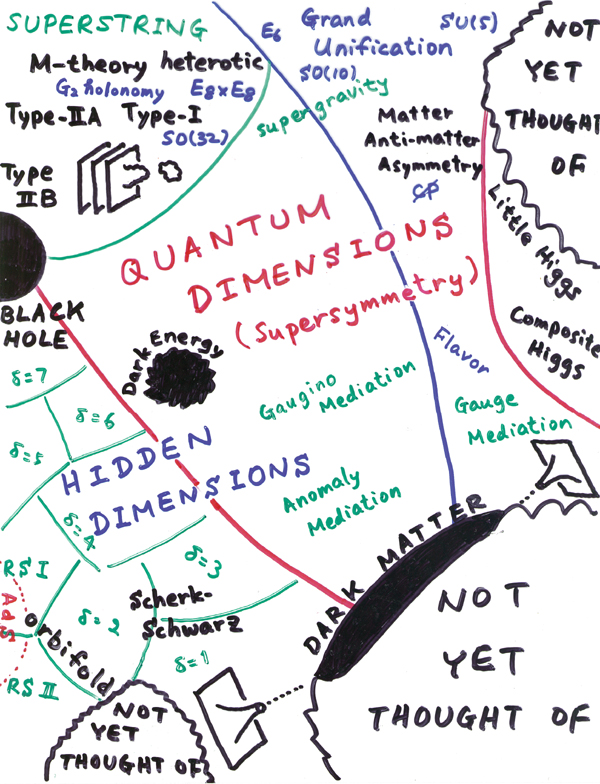
\includegraphics[width= 0.75\textwidth]{./assets/particlephysics}\\ {\tiny  dailygalaxy.com}
		\column{.5\textwidth}
		\begin{center}
			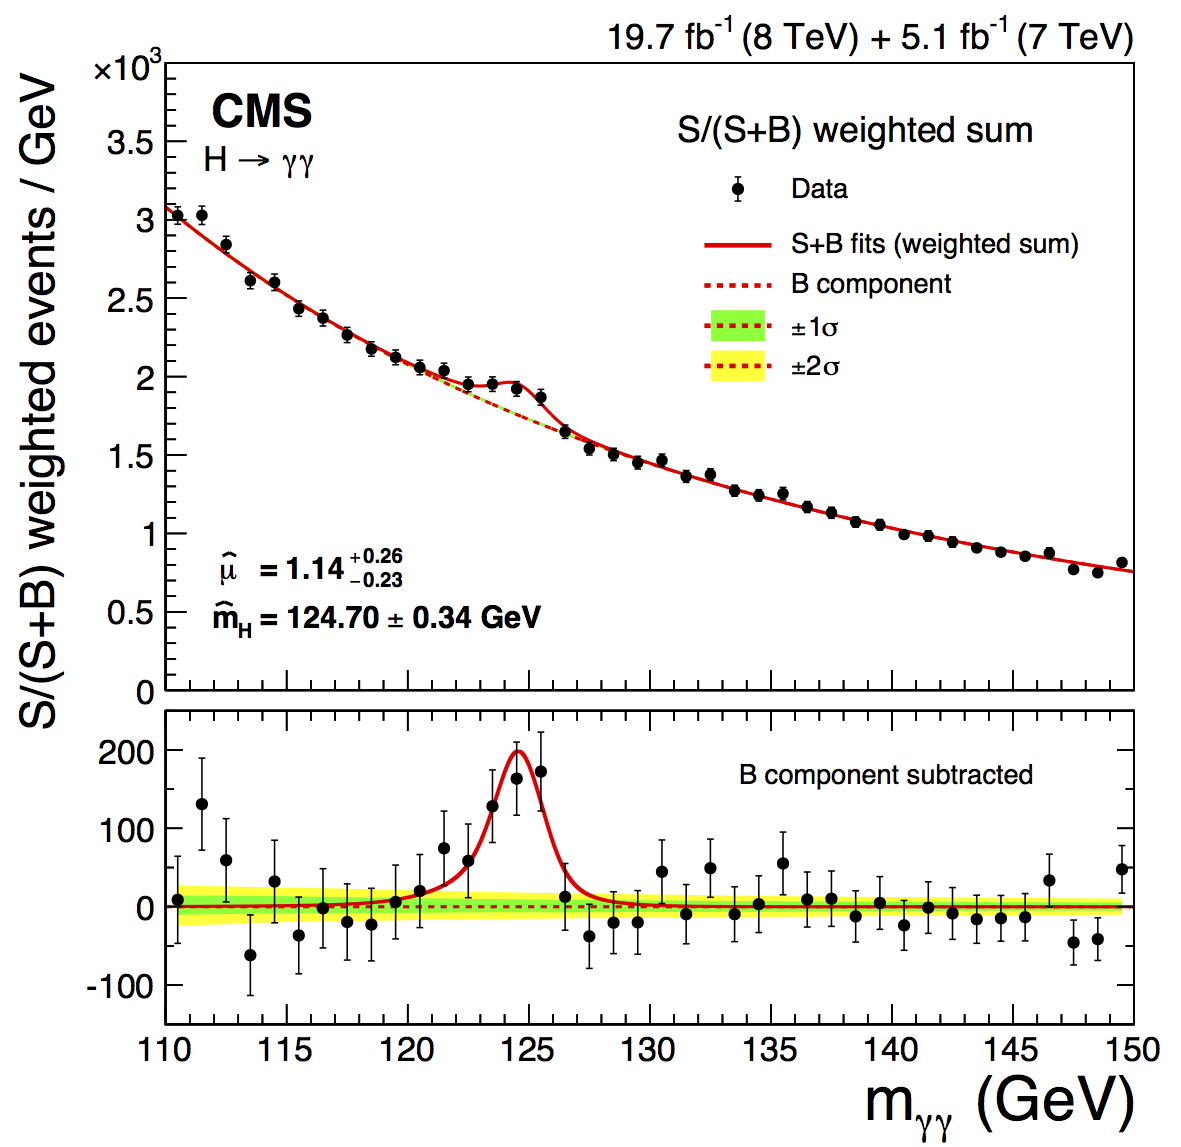
\includegraphics[width= 0.55\textwidth]{./assets/higgs}\\
			{\tiny \arXivCode{1207.7235 }}\\
			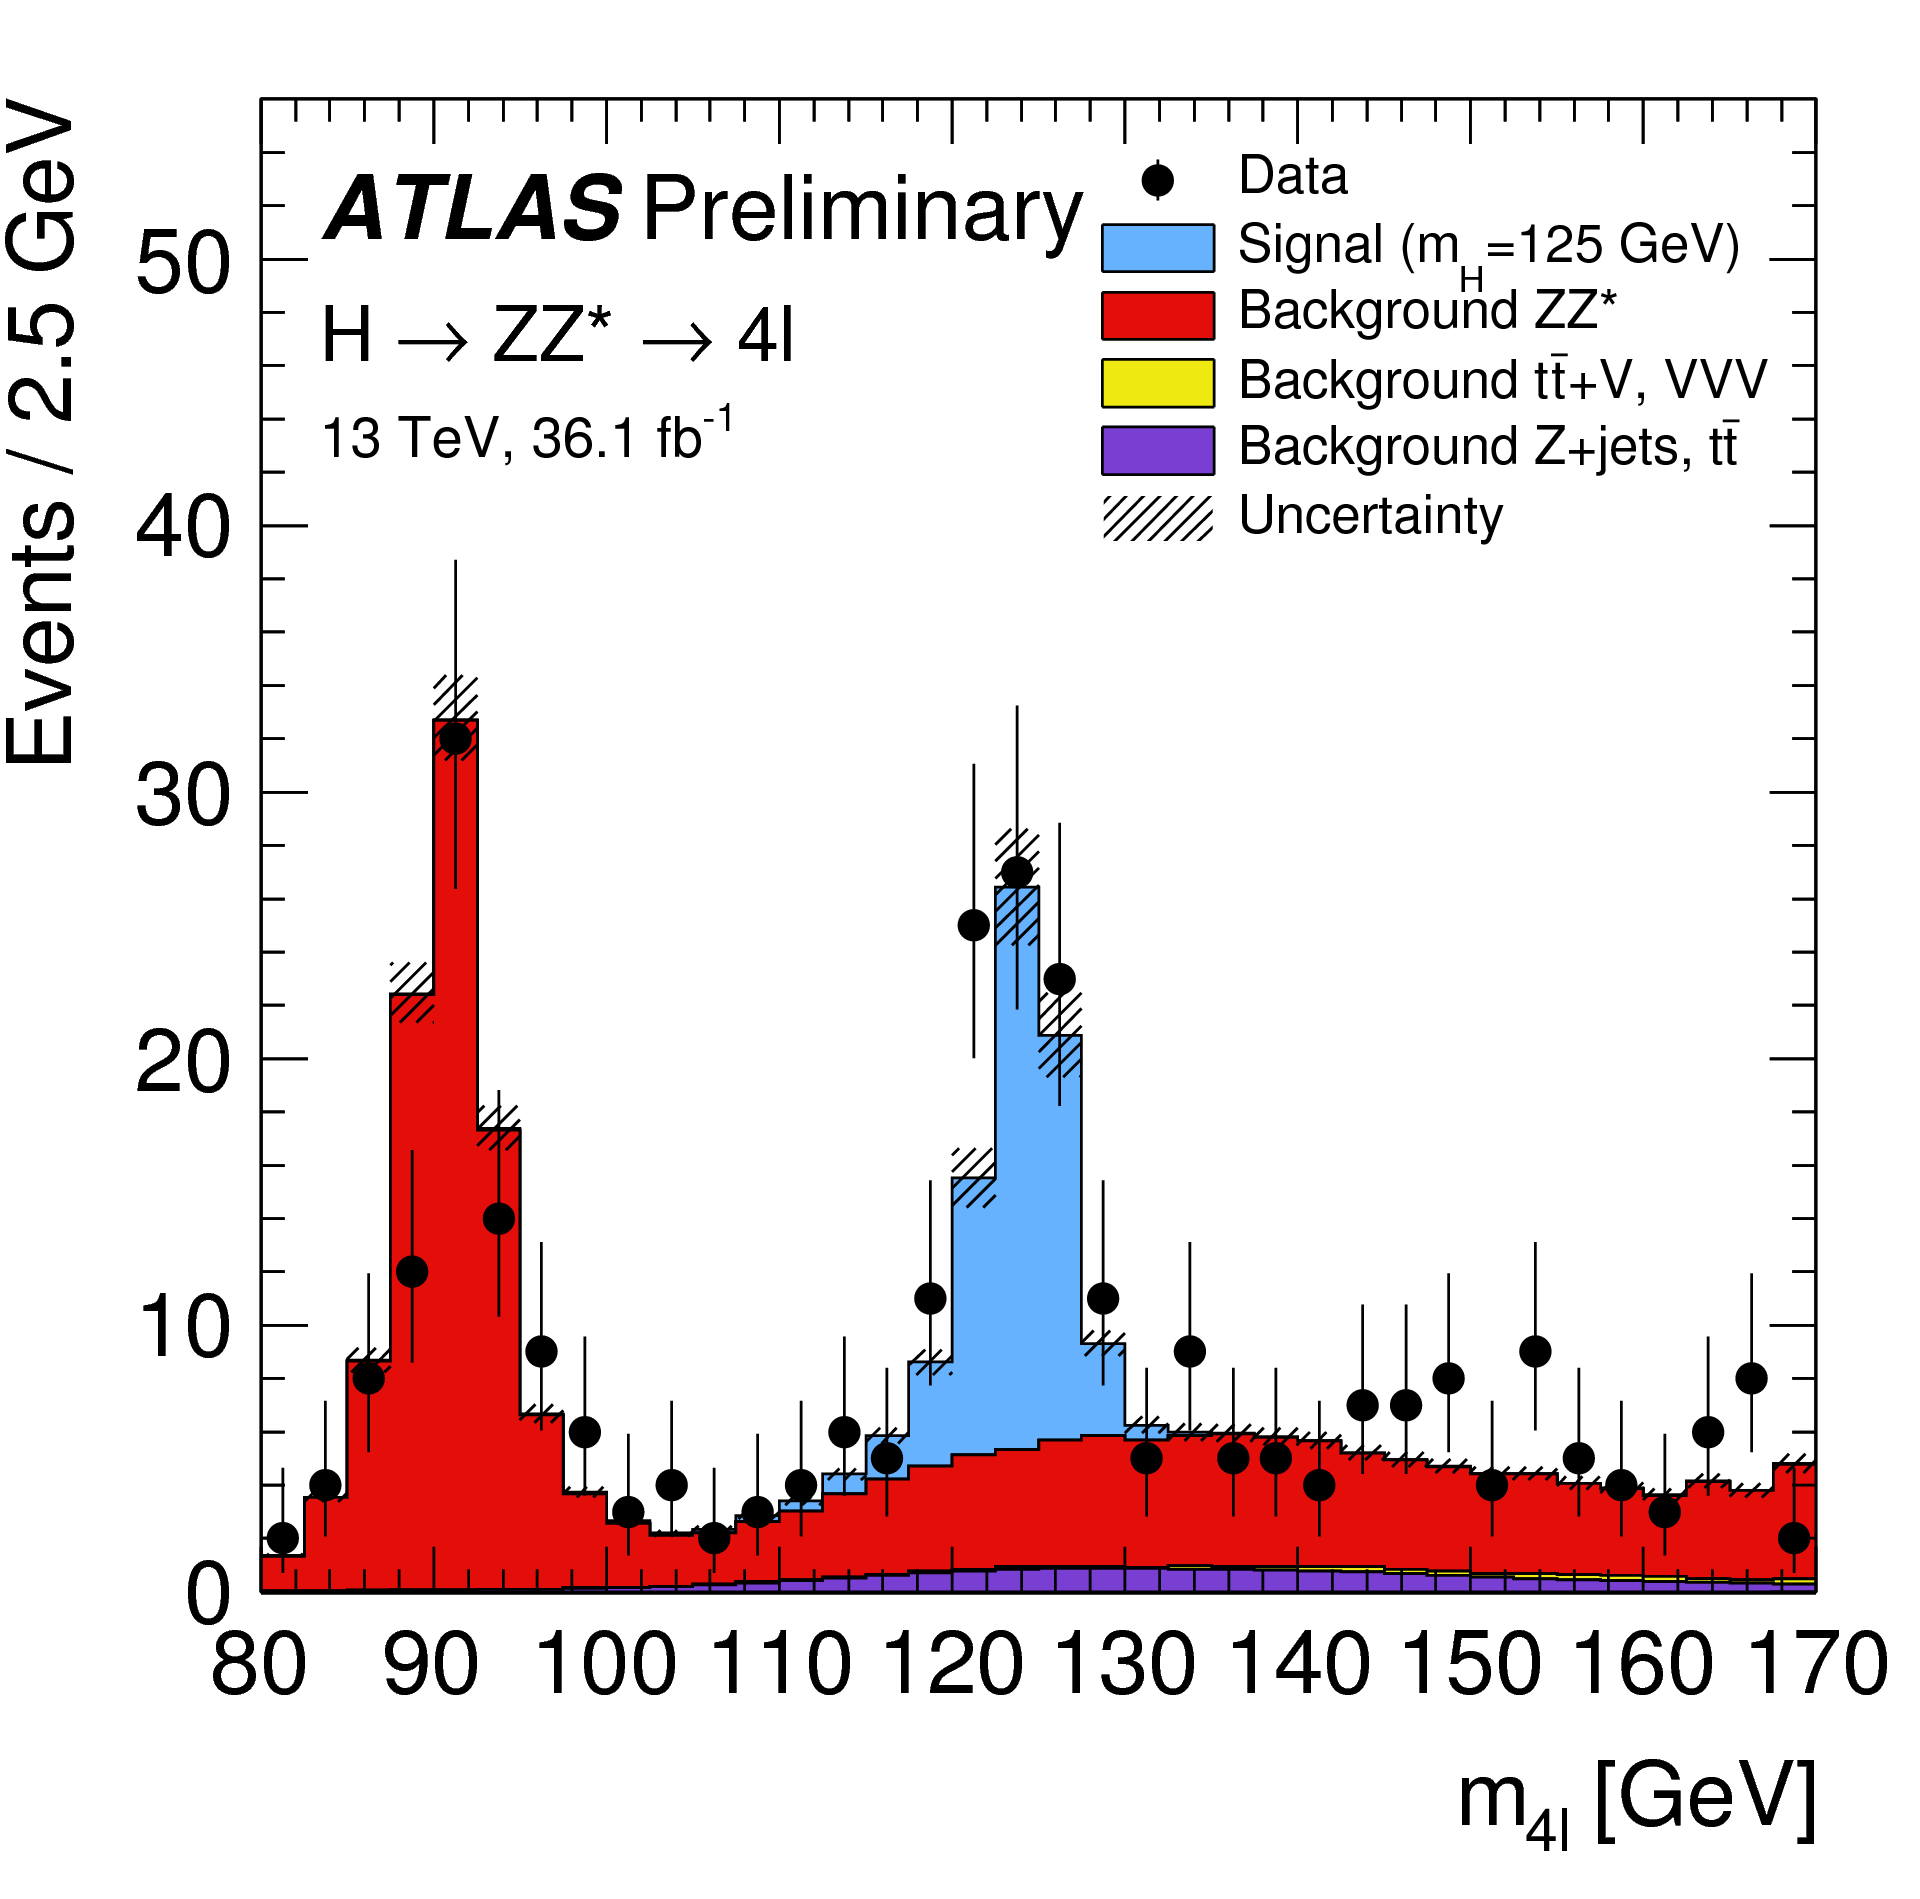
\includegraphics[width= .55\textwidth]{./assets/higgs-1} \\
			{\tiny ATLAS-CONF-2017-032}
		\end{center}
	\end{columns}
\end{frame}

%===========================================================
% Slide 2
%===========================================================

\begin{frame}{$B_{s} \to \mu \mu$ }
The heavily suppressed~ (in the  SM) decay $ B_s \to \mu \mu$ was first seen by a joint effort between CMS and \LHCb in 2015.
	\begin{columns}[c]
		\column{.5\textwidth}
		\centering
		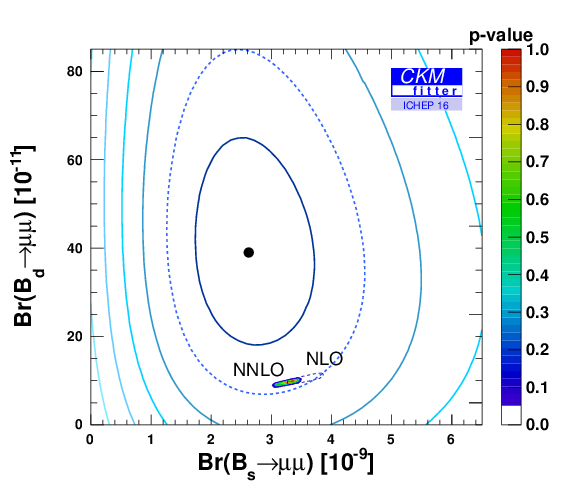
\includegraphics[width= \textwidth]{./assets/BsBdtomumu}\\ {\tiny CKM-fitter}
		\column{.5\textwidth}
Later in 2017 \LHCb measurement was made with $ 7.8 \sigma$ significance !
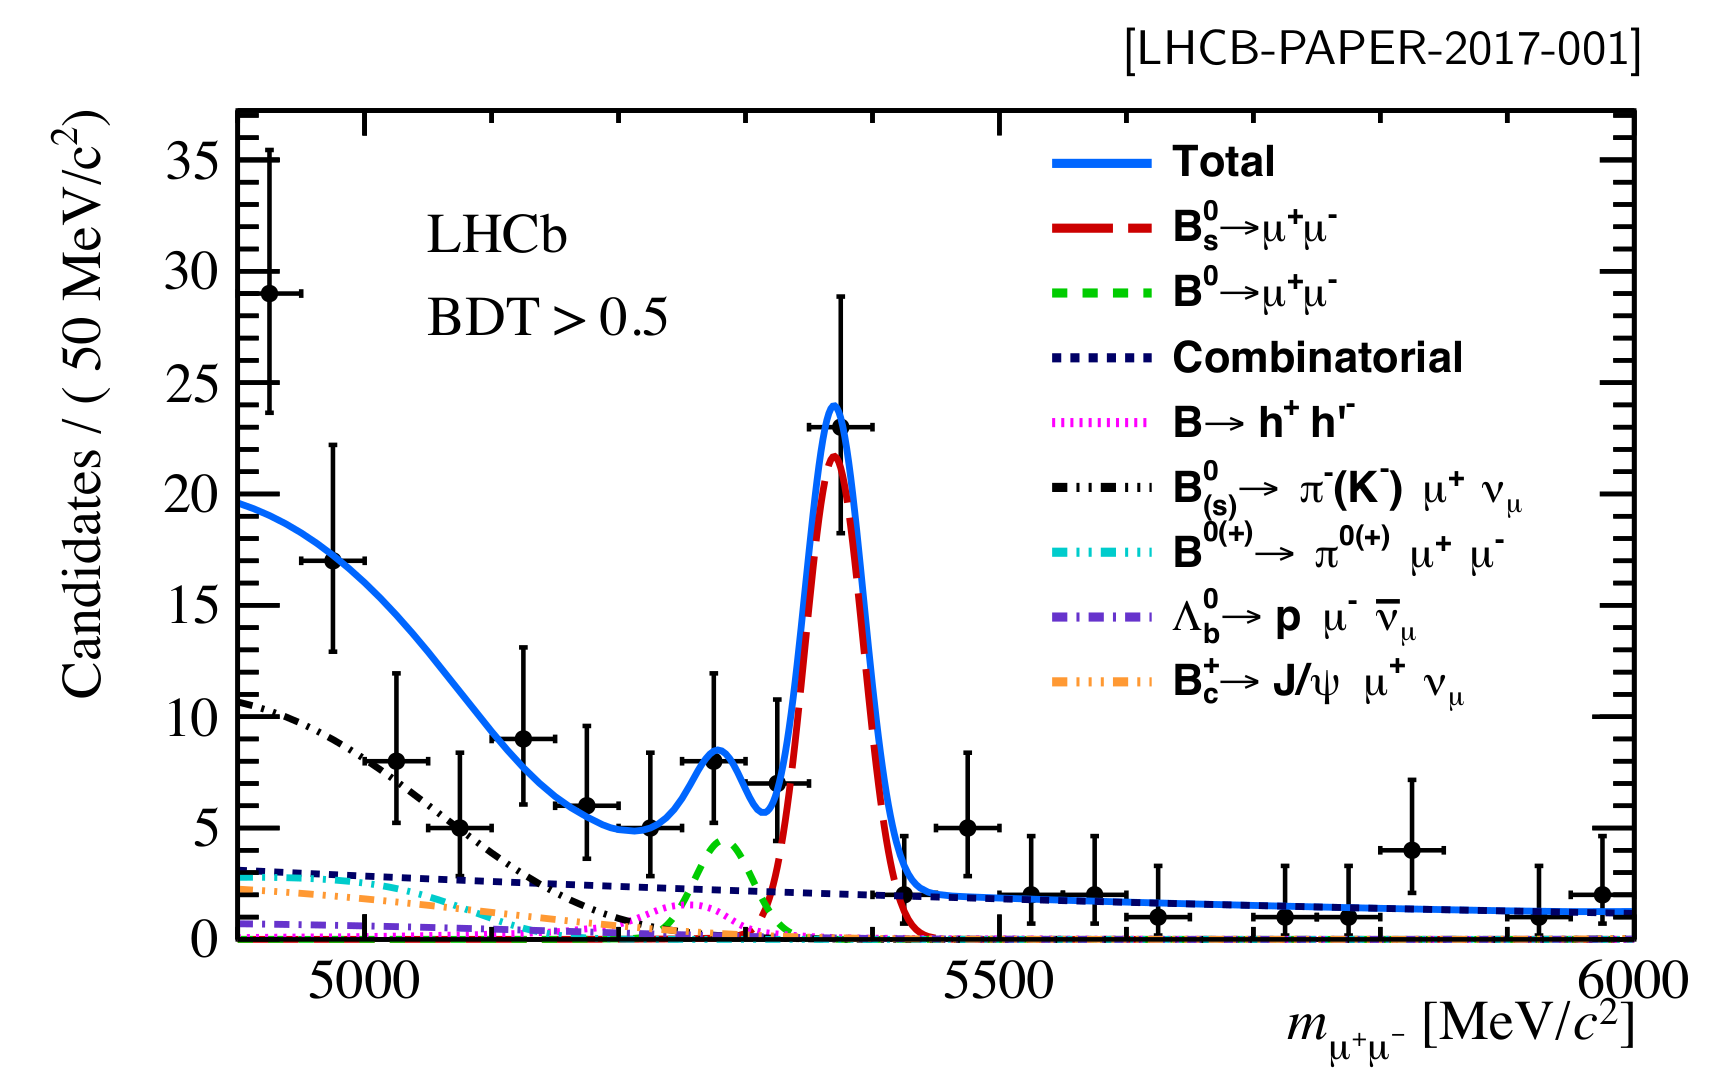
\includegraphics[width= 1.1\textwidth]{./assets/bsmumu_2017_LHCb} \\ {\tiny \arXivCode{1703.05747  }}
	\end{columns}
\end{frame}
%===========================================================
% Slide 3
%===========================================================
\begin{frame}{Precision measurements}
	\begin{columns}[c]
		\column{.3\textwidth}
		Various parameters sensitive to NP from heavy flavour physics, the pull is estimated from the SM global fit\\ Results show consistency with the SM in general ..
		\column{.7\textwidth}
		\centering
		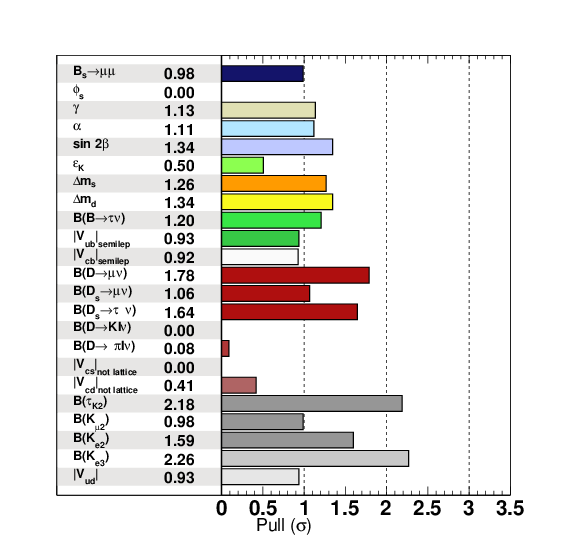
\includegraphics[width= \textwidth]{./assets/Pulls}\\ (CKM Fitter group)
	\end{columns}
\end{frame}
%===========================================================
% Slide 4
%===========================================================
\begin{frame}{It is not as dark as it seems ! {\small or is it ??}}
	\begin{columns}[c]
			\column{.5\textwidth}
			\centering
			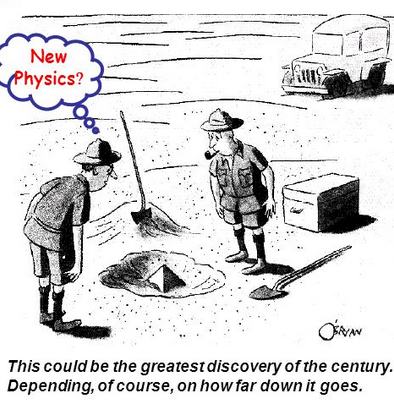
\includegraphics[width= \textwidth]{./assets/NP}\\{\tiny SLAC DOE Rev. 2006}
	\column{.5\textwidth}
Few years ago, some hints from B-factories and the \LHCb started showing tension between beauty physics and the SM
	
	\end{columns}
\end{frame}
%===========================================================
% Slide 5
%===========================================================
\begin{frame}{Lepton Universality in the SM}
If we examined  the lepton coupling to the $Z$ and $ W^\pm$ via measurement of the branching fractions~$\mathcal B$ of the leptonic decays of the $Z$ produced in $ee$ collisions for any two of the three families, it has been measured to be close to unity~(i.e.$ \sim 1$).
	\begin{columns}[c]
		\column{.5\textwidth}
		\begin{align*}
			\mathcal B (Z \to e^+ e^-) &= (3.363 \pm 0.004) \% \\
			\mathcal B (Z \to \mu^+ \mu^-)  &= (3.366 \pm 0.007) \% \\
			\mathcal B (Z \to \tau^+ \tau^-)  &= (3.370 \pm 0.008) \% 
		\end{align*}
		\column{.5\textwidth}
		\begin{align*}
			\mathcal B (W^+ \to e^+ \nu)  &= (10.75 \pm 0.13) \% \\
			\mathcal B (W^+ \to \mu^+\nu )  &= (10.57 \pm 0.15)\% \\
			\mathcal B (W^+\to \tau^+ \nu)  &= (11.25\pm 0.20 )\% 
		\end{align*}	
	\end{columns}
	{\tiny PDG 2016}\footnote{ The $ W \to \tau \nu$ is  $\sim 1 \sigma$ higher than the other due to the chirality and D- functions \\ The SM prediction is 10.75 \%}
\end{frame}
%===========================================================
% Slide 6
%===========================================================
\begin{frame}{Lepton universality in quark transitions}
	\begin{columns}[c]
		\column{.5\textwidth}
	Quark transitions in beauty and charmed hadrons decays offer an additional  test for the Lepton Flavour Universality~(LFU). By the FCCC in the $ b\to c$ transition and FCNC penguins  in~$ b \to s$ transition.
		\column{.5\textwidth}
		\begin{center}
			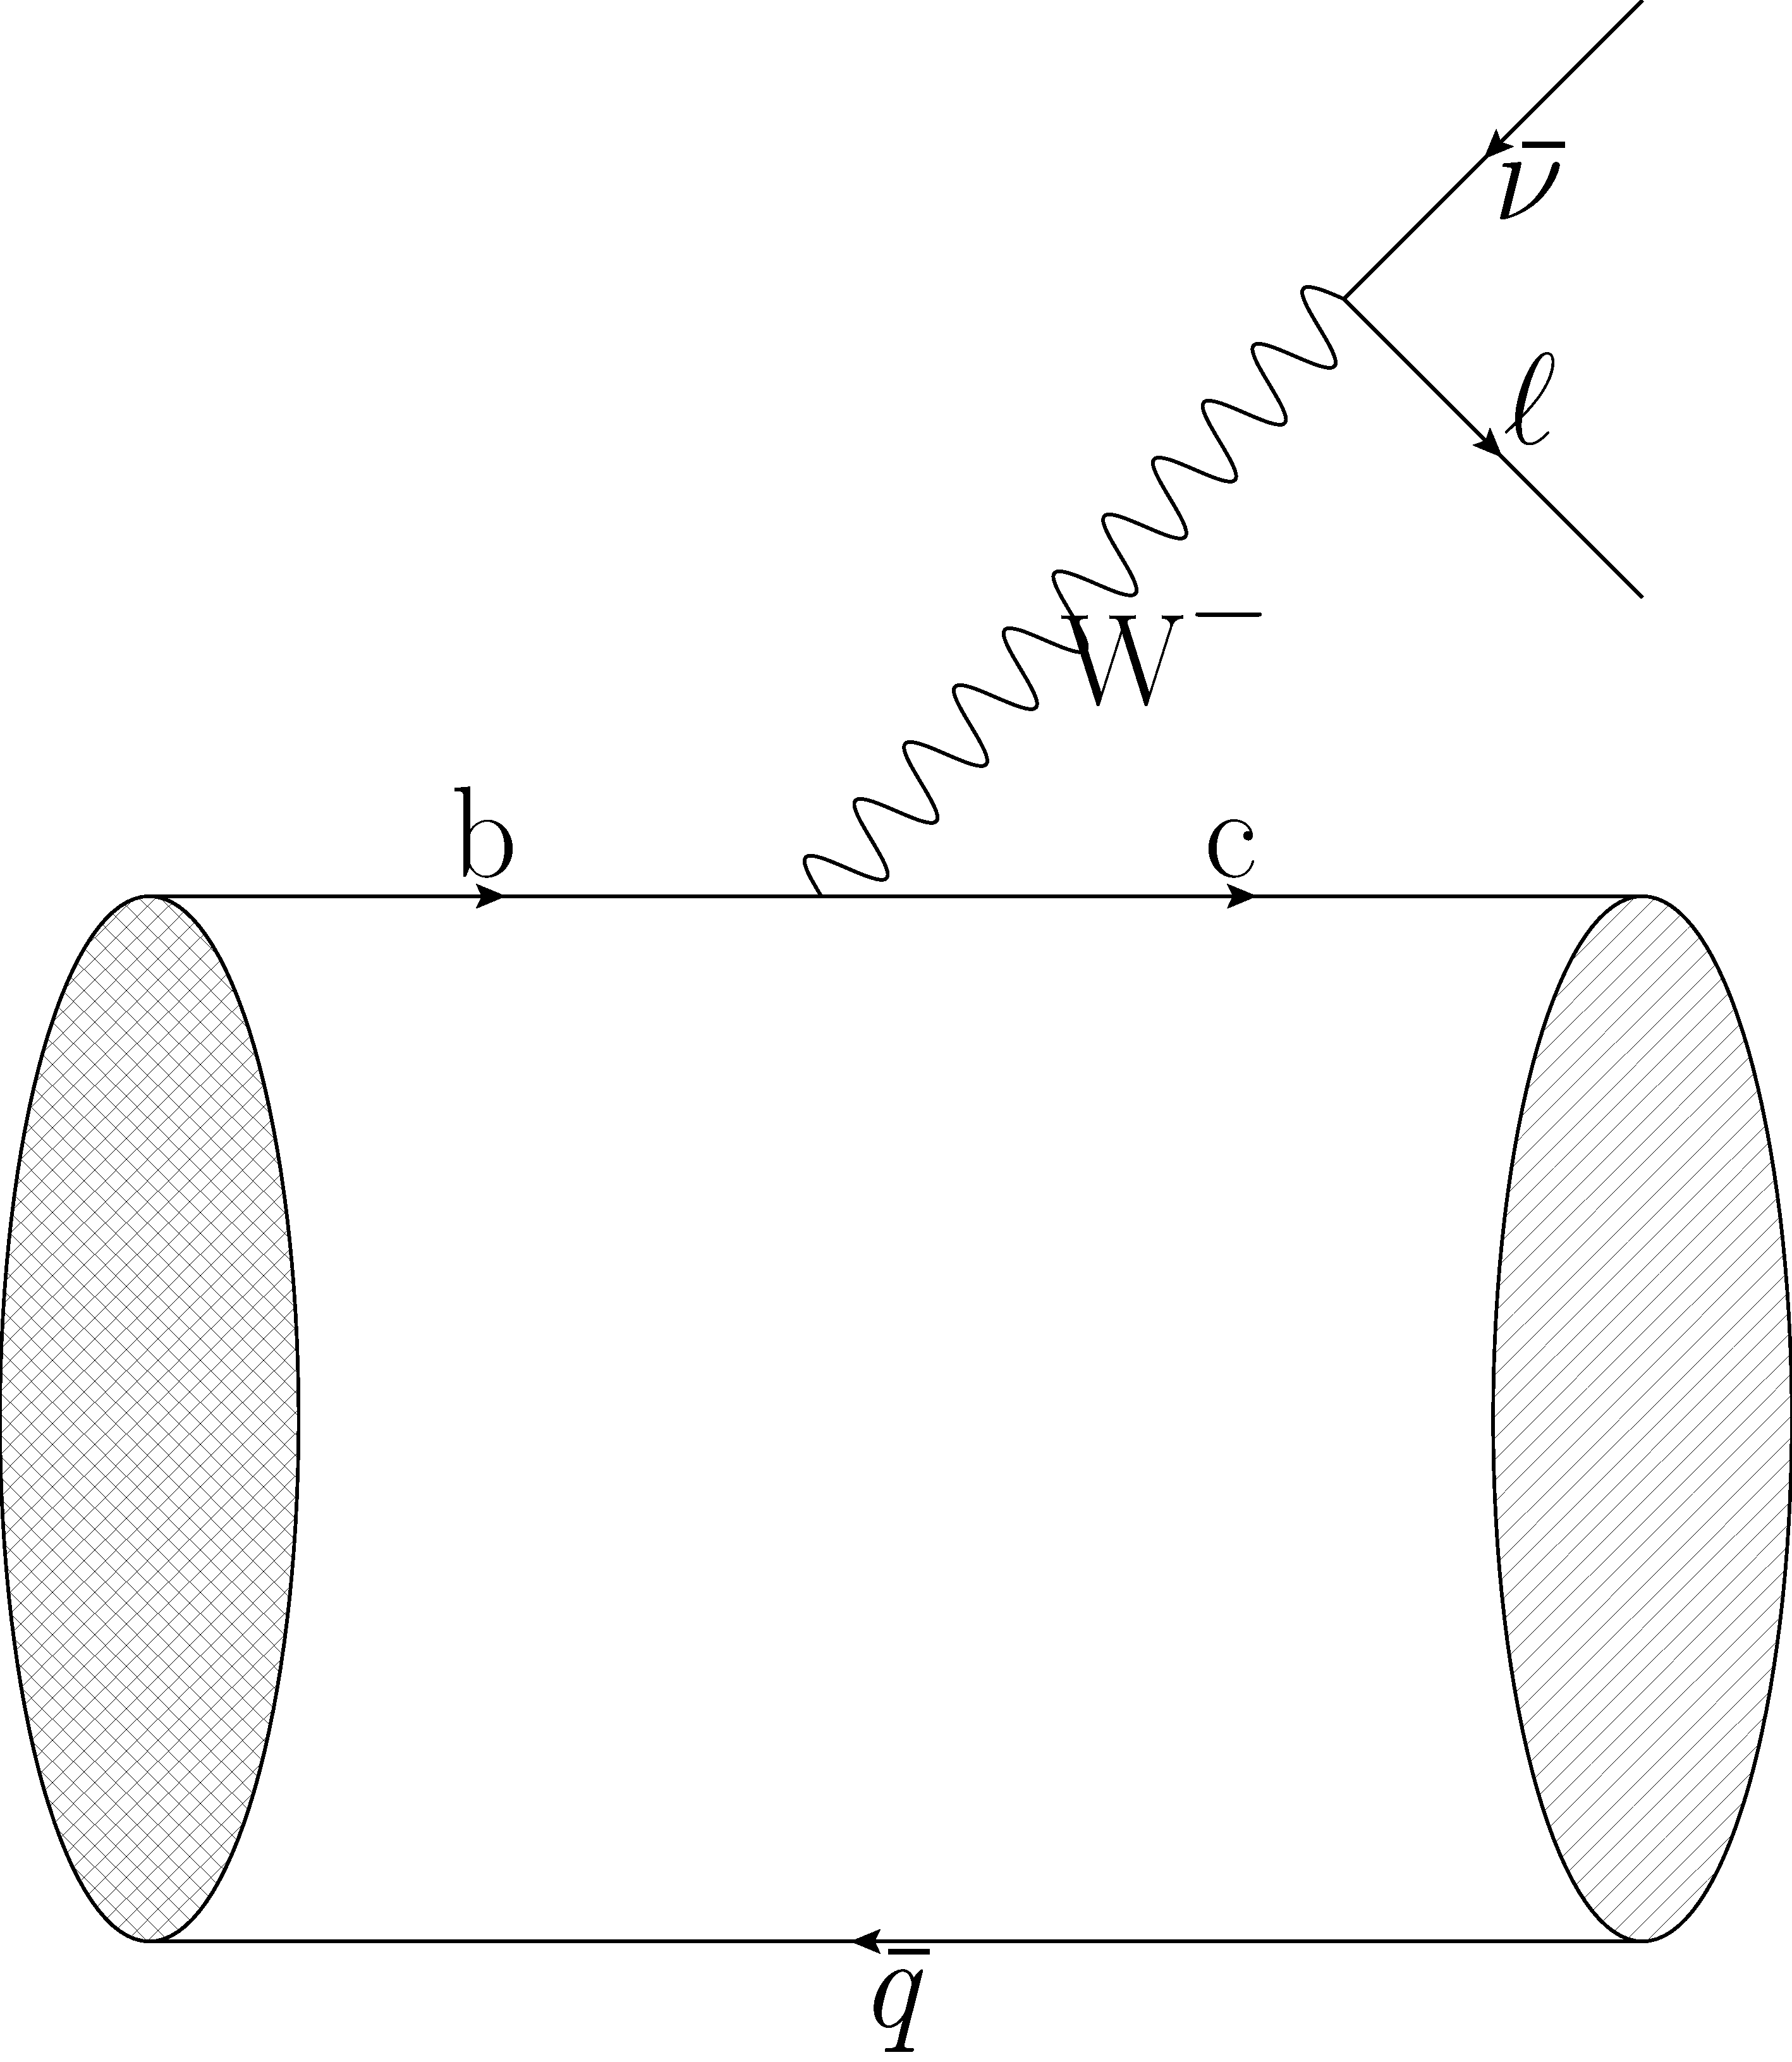
\includegraphics[width=0.5 \textwidth]{./assets/B_to_D_SM}\\
			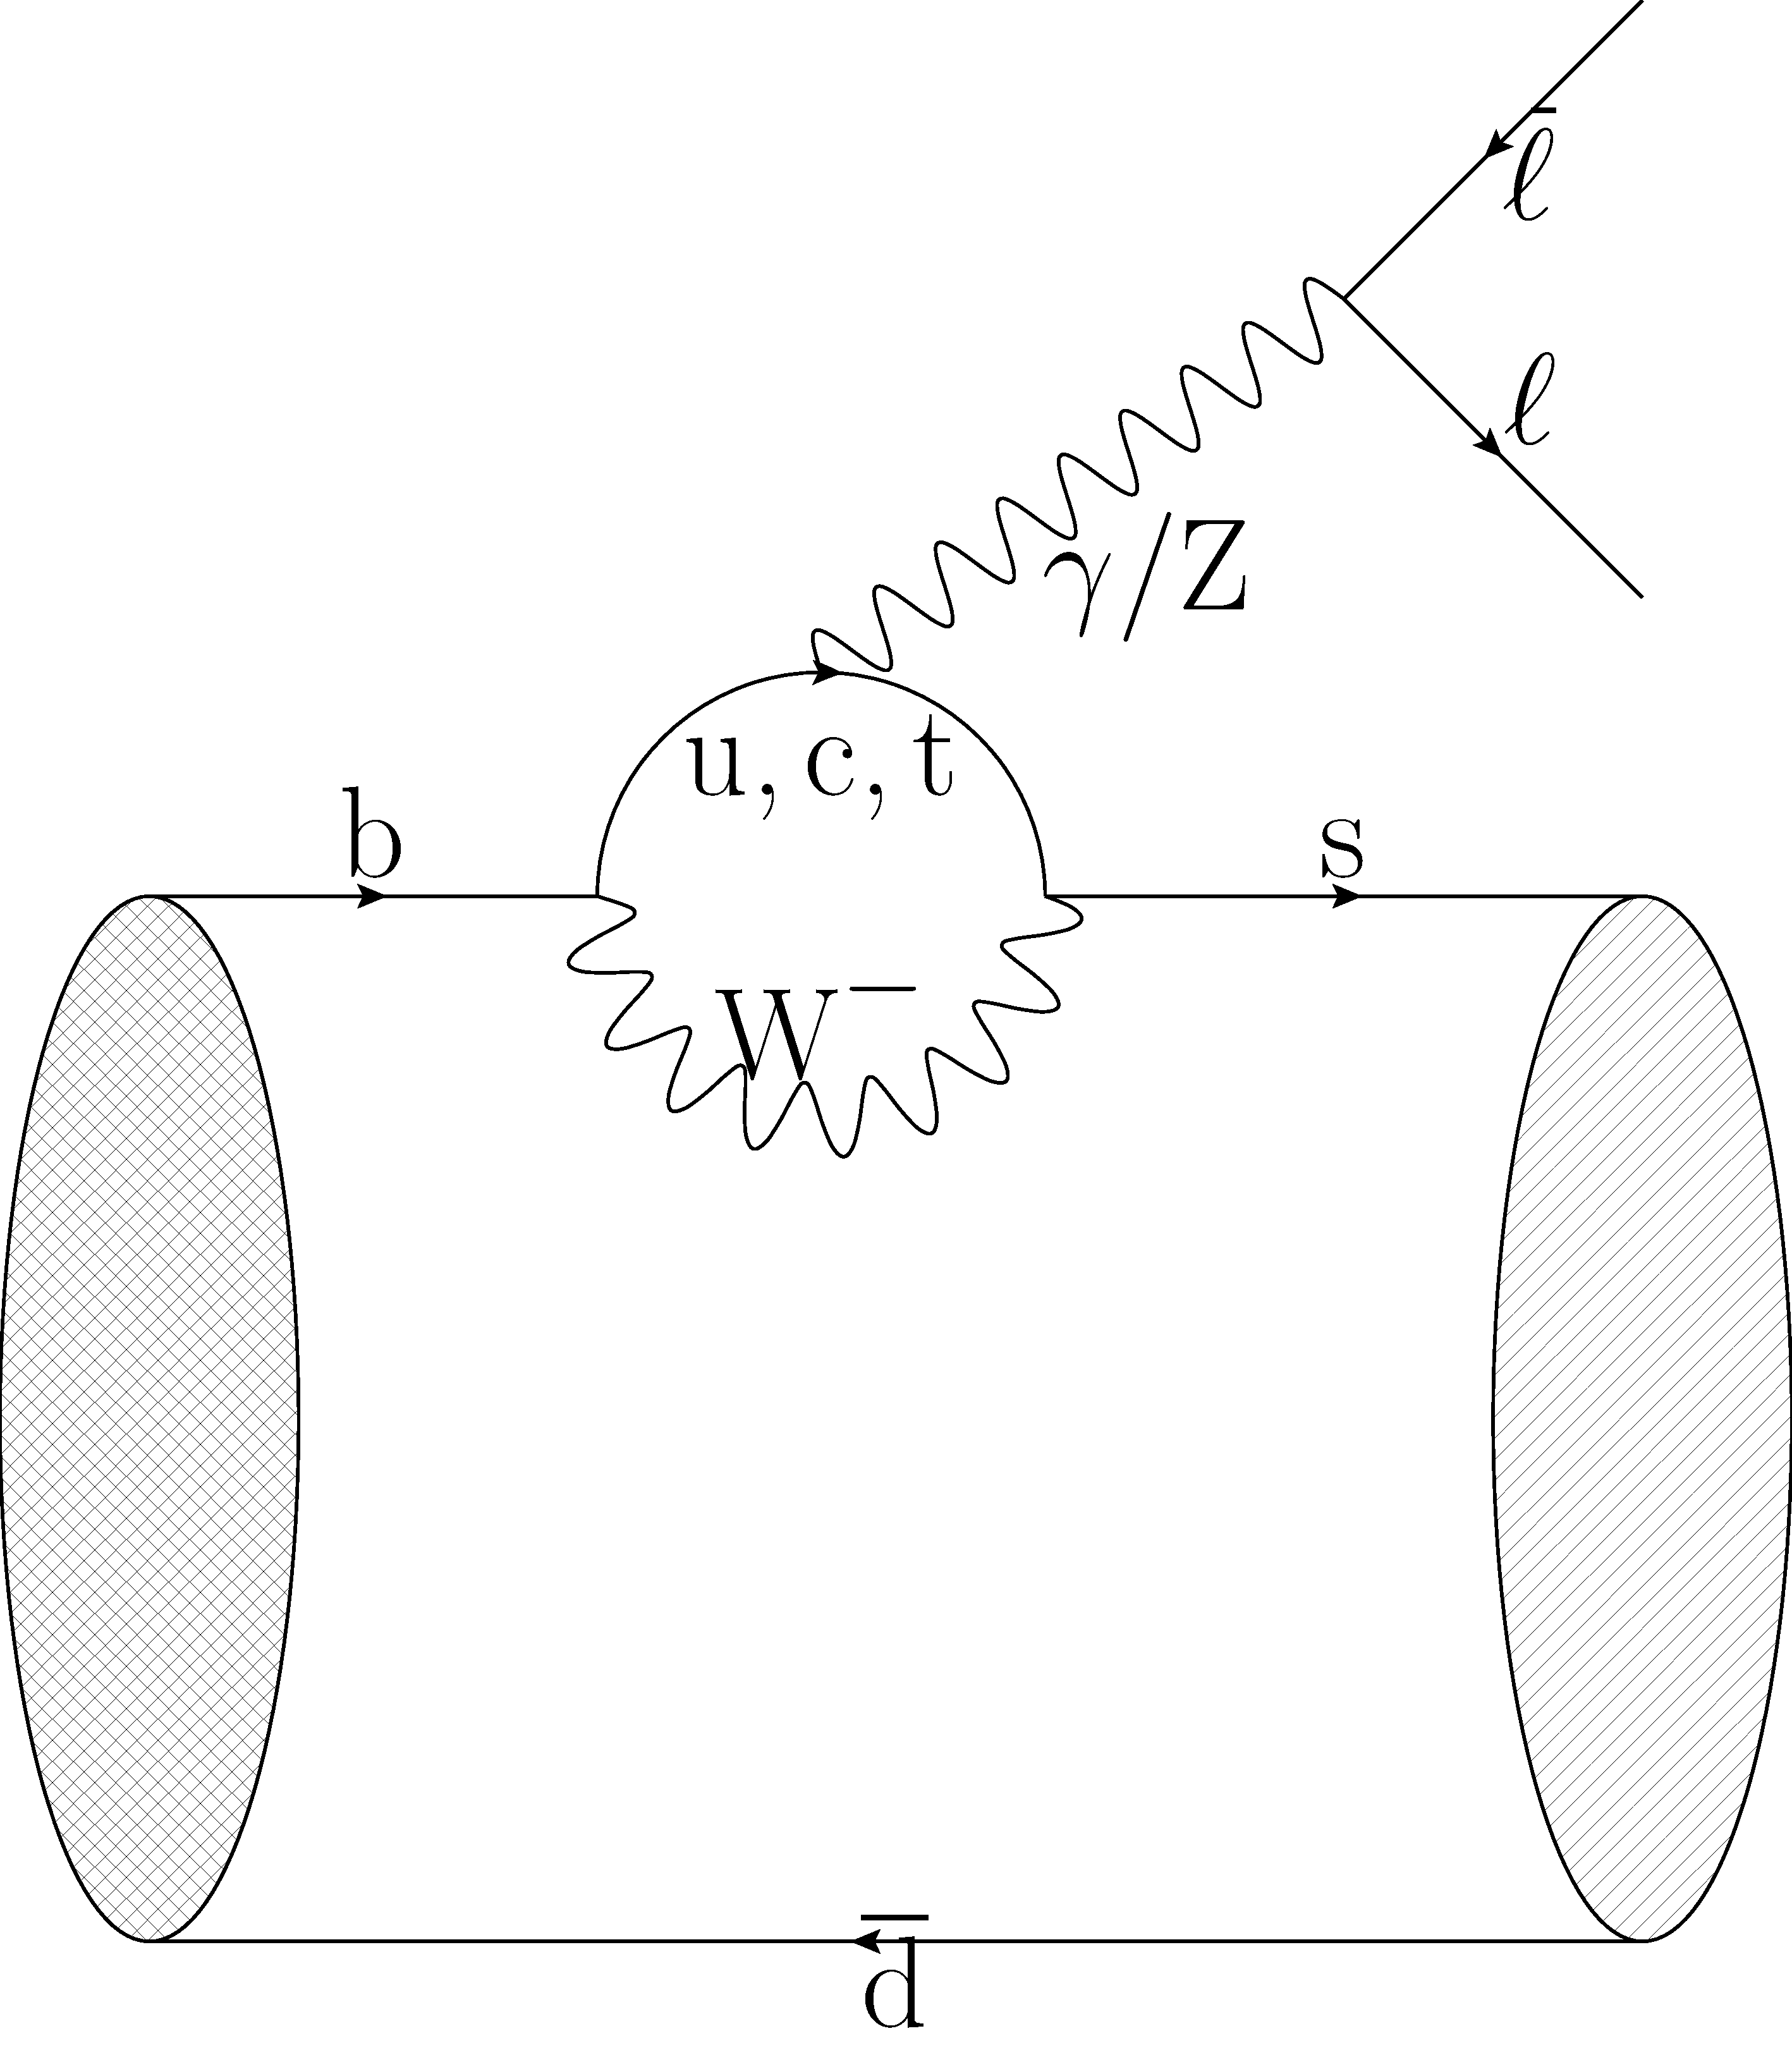
\includegraphics[width= 0.5\textwidth]{./assets/B_to_K_SM} 
		\end{center}
	\end{columns}
\end{frame}%
%===========================================================
% Slide 7
%===========================================================
\begin{frame}{ Hints of LFU violation}
	Tests for LFU using the $B$ meson decays involving the quark transitions 
	$ b\to c \;\mu \nu$ and $ b\to c \;\tau \nu$, via the observables
	\begin{equation*}
	R_{D^{(*)}} \equiv \frac{\mathcal B (\bar B \to D^{(*)} \tau ^- \bar \nu)}{\mathcal B (\bar B \to D^{(*)} \ell ^- \bar \nu)},
	\end{equation*}
	has reported an average of $\sim 4 \sigma$ deviation from Standard Model predictions.
	\begin{figure}
		\centering
		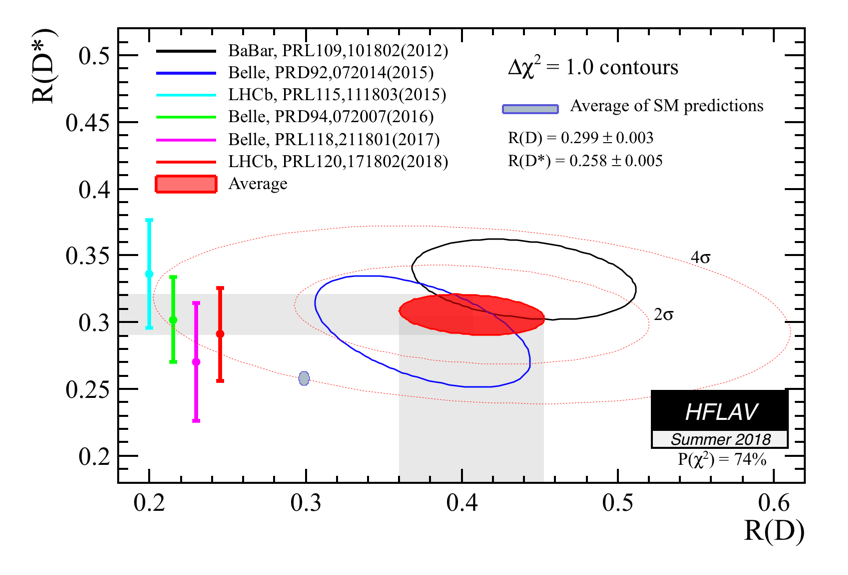
\includegraphics[width=.65 \textwidth]{./assets/rdrds_summer18} \\
		{\tiny Heavy Flavour Averaging  Group (CERN- 2018)}
	\end{figure}
\end{frame}
%===========================================================
% Slide 8
%===========================================================
\begin{frame}{ Hints of LFU violation}
	LHCb measurements of the observables:
	\begin{equation*}
	R_{K^{(*)}} \equiv \frac{\mathcal B (\bar B \to K^{(*)} \mu \mu)}{\mathcal B (\bar B \to K^{(*)} ee)},
	\end{equation*}
	that involve the quark transitions, 
	$ b\to s \;ee$ and $ b\to s\; \mu \mu$. 
	\begin{columns}[c]
		\column{.5\textwidth}
		\begin{center}
			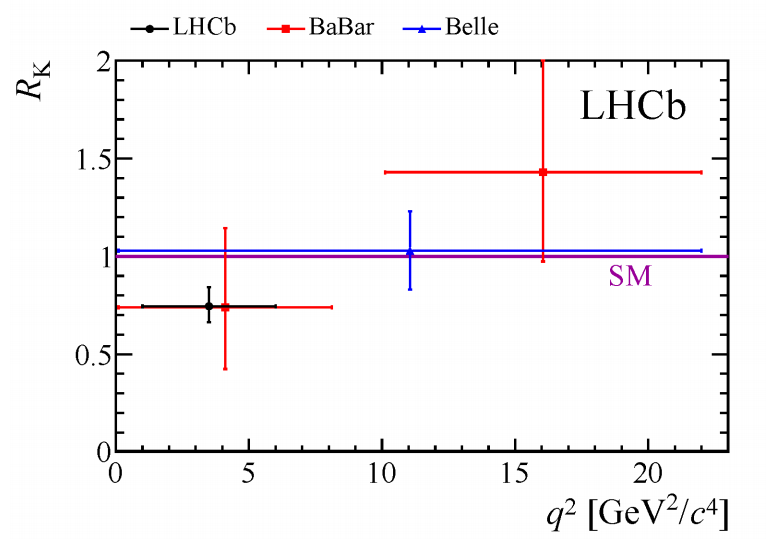
\includegraphics[width= \textwidth]{./assets/RK}\\ {\tiny \arXivCode{1406.6482  }} 
		\end{center}
		\column{.5\textwidth}
		\begin{center}
			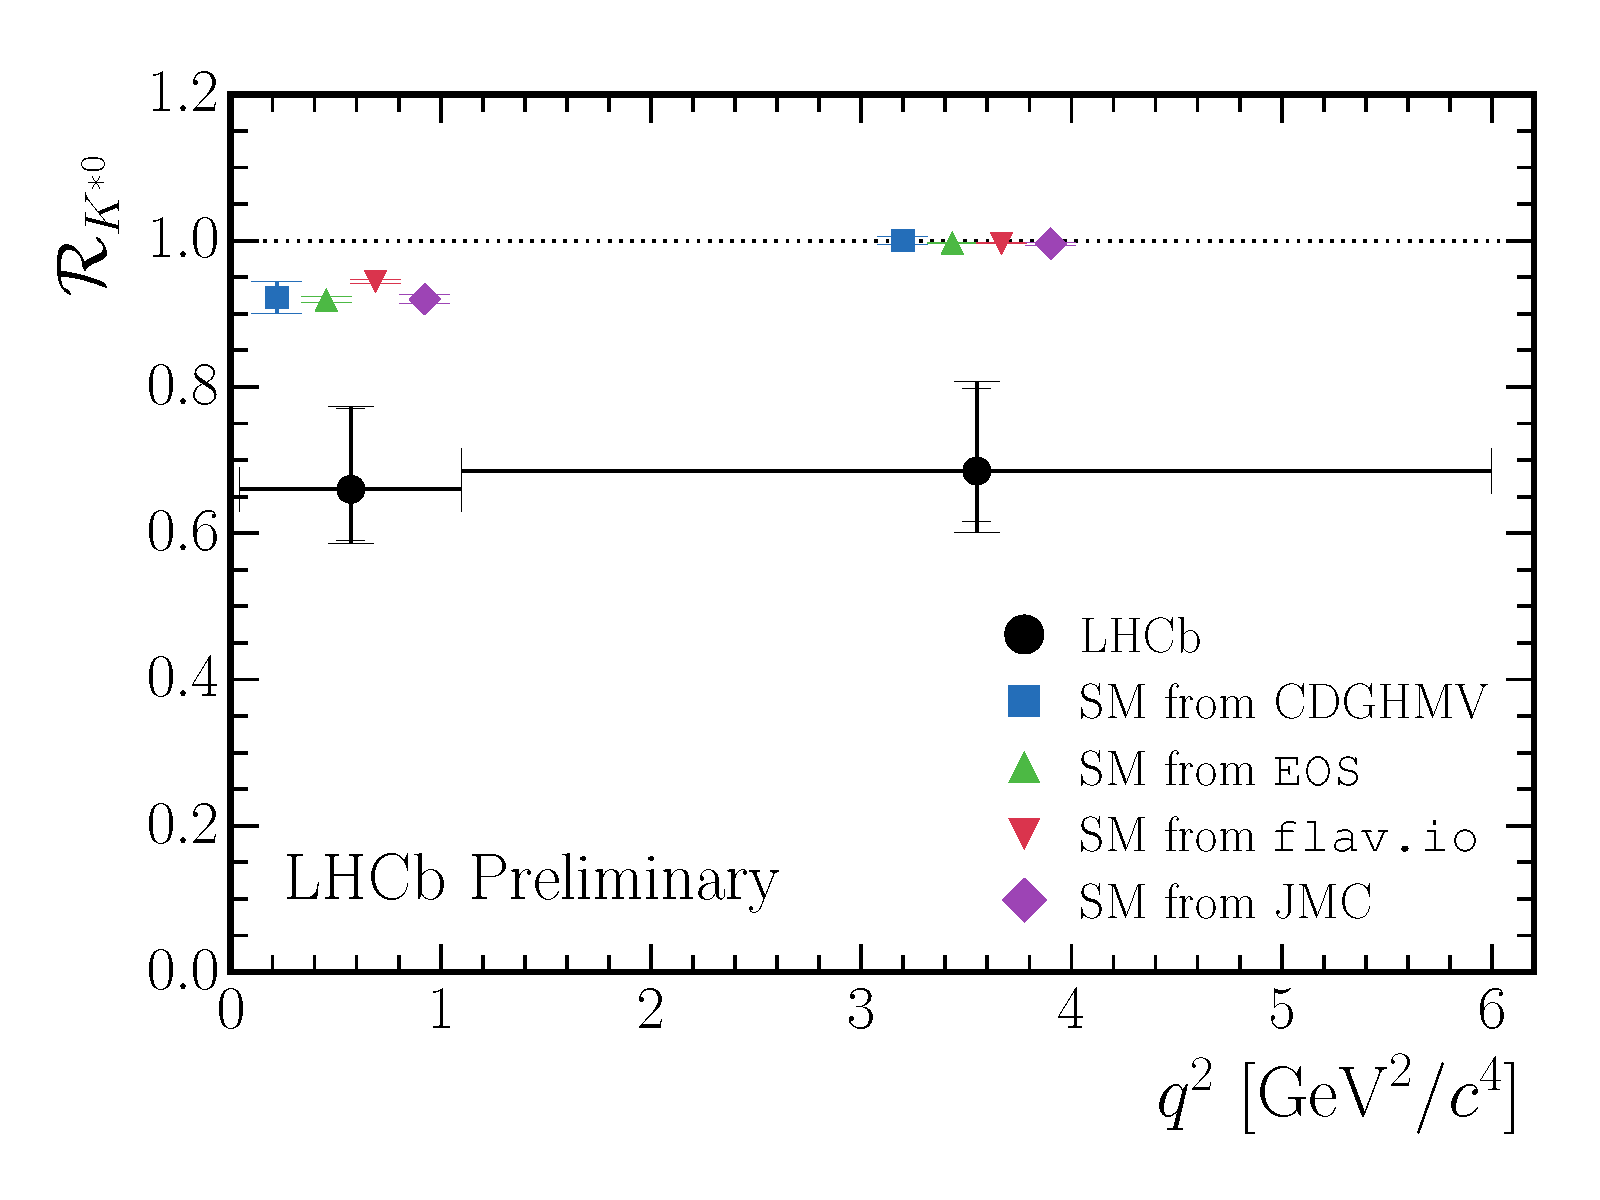
\includegraphics[width= \textwidth]{./assets/RKstar} \\ {\tiny \arXivCode{1705.05802  }} 
		\end{center}
	\end{columns}
	Shows  SM deviation of $2.2-2.4 \sigma$ at low  and $ \sim 2.6 \sigma$ at central $q^2$ for $R_{K^{*}}$ \\
	$R_{K}$ has shown a $ \sim 2.5\sigma$ deviation from SM prediction from \LHCb measurements .
\end{frame}%
%===========================================================
% Slide 9
%===========================================================
\begin{frame}{Angular analysis of $ B \to K^* \mu^+ \mu^-$ }	
	\begin{columns}[c]
		\column{.5\textwidth}
		Clean observables, with small hadronic uncertainty.
		\begin{center}
			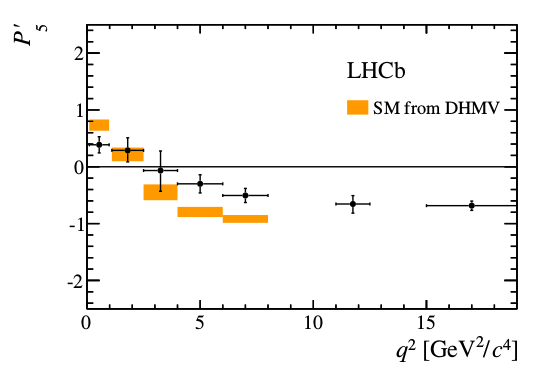
\includegraphics[width= \textwidth]{./assets/pp_5_lhcb}\\ $3.7 \sigma$ from SM
		\end{center}
		\column{.5\textwidth}
		\begin{center}
			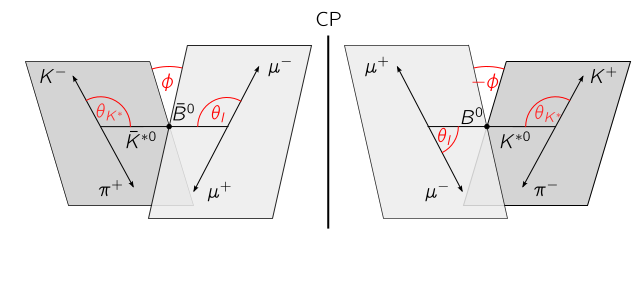
\includegraphics[width= \textwidth]{./assets/pp_5.png} \\ 	{\tiny \arXivCode{1512.04442}}
		\end{center}
		\begin{center}
			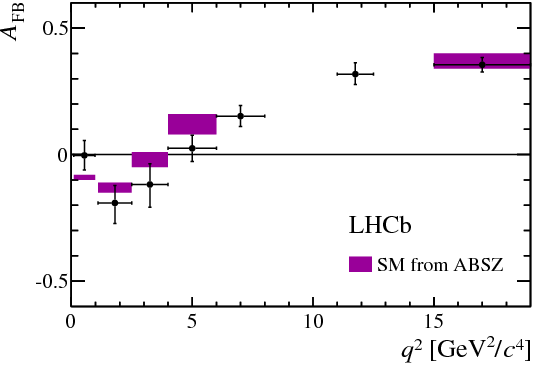
\includegraphics[width= \textwidth]{./assets/figs_averages_AFBPad} 
		\end{center}
	\end{columns}
\end{frame}
%===========================================================
% Slide 10
%===========================================================
\begin{frame}{Differential branching fractions}	
	\begin{columns}[c]
		\column{.5\textwidth}
	The angular analysis was preformed on $ B_s \to \phi(K^+K^-) \mu^+\mu^-$, as it has similar helicity states expansion as  $ B \to K^* \mu^+ \mu^-$, the angular observables tuned to be consistent with SM, but the dif. BR was found to be $ > 3 \sigma$ less than the SM prediction.\\
	\begin{center}
		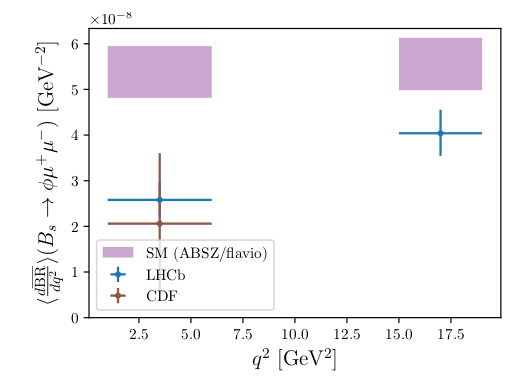
\includegraphics[width= 0.9\textwidth]{./assets/btophimumu} \\ {\tiny \arXivCode{1506.08777}}
	\end{center}
		\column{.5\textwidth}
		Similar deviation could be seen in other BR involving $b \to s \mu \mu $.\\
		\begin{center}
			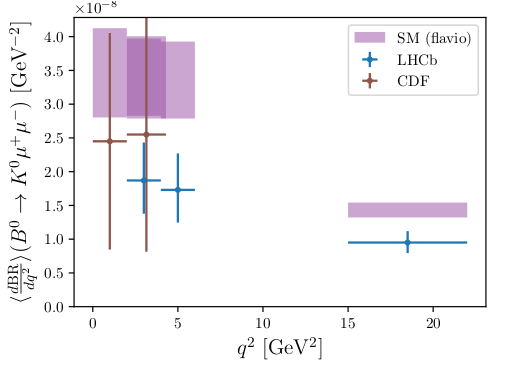
\includegraphics[width=0.8\textwidth]{./assets/btokmumu} \\
			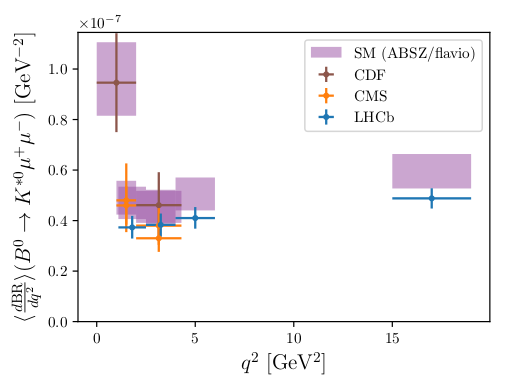
\includegraphics[width=0.8\textwidth]{./assets/tokstarmumu}
		\end{center}
	\end{columns}
	{\small Plots by D. Straub - \texttt{flav.io}}
\end{frame}
%==========================================================
% Slide 11
%===========================================================
\begin{frame} {Differential branching fractions}
	\begin{columns}[c]
		\column{.4\textwidth}
More discrepancies can be seen in other decays involving~$ b \to s\mu \mu $ transitions branching fractions, suggesting that the $\mu$ is the source of the LFU anomalies not the $e$.  
		\column{.6\textwidth}
		\begin{center}
			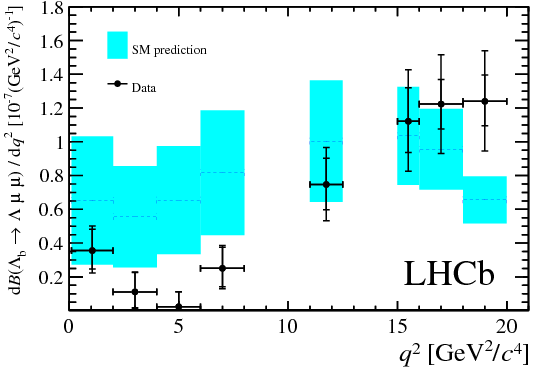
\includegraphics[width= 0.75\textwidth]{./assets/figure5} \\ {\tiny \arXivCode{1503.07138 }}  
				\begin{center}
					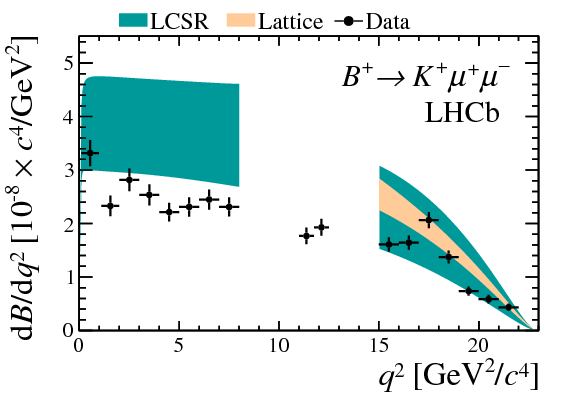
\includegraphics[width=0.75 \textwidth]{./assets/kmumu_BF} \\ 
				\end{center}
		\end{center}
	\end{columns}
\end{frame}
%===========================================================
% Slide 12
%===========================================================
	\begin{frame}{Understanding the source of $ b\to s \mu \mu$ anomalies }
One could argue that such discrepancies come from hadronic uncertainties or that we are missing something in qcd processes beyond form factors.. but this is apparently not the case.\\
	\begin{center}
		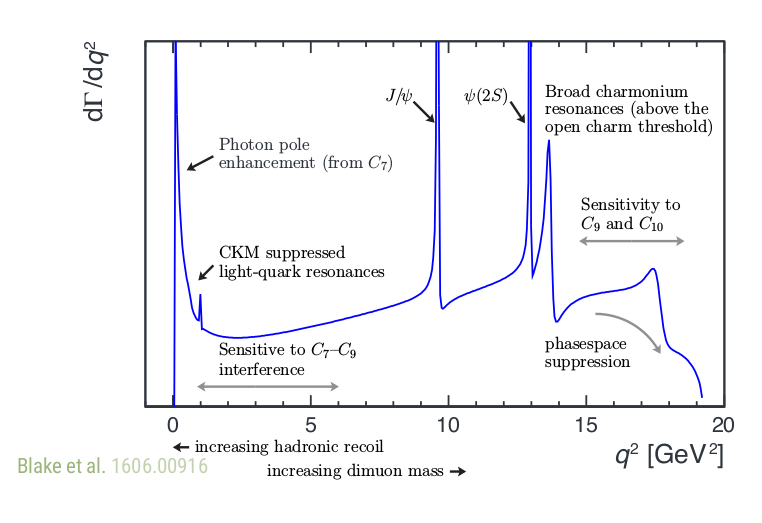
\includegraphics[width= 0.8\textwidth]{./assets/q2_bkll} 
	\end{center}
	\end{frame}
%===========================================================
% Slide 13
%===========================================================
\begin{frame}{Global fits for $ b \to s \ell \ell$}
	\begin{columns}[c]
		\column{.5\textwidth}
		\begin{center}
			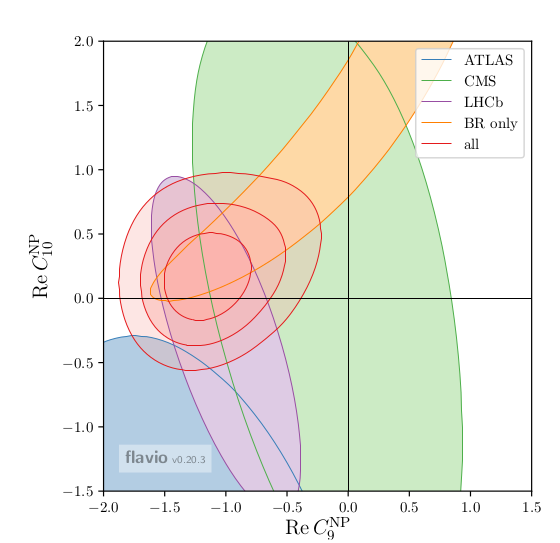
\includegraphics[width=0.9 \textwidth]{./assets/c9_c10}\\ $5\sigma$
		\end{center}
		When we combine all of these effects in terms of Wilson coefficients, and pull them from $SM$ by:
		\[\text{pull} = \sqrt{\chi_{SM}^2-\chi_{\text{best fit}}^2}  \] 
		\column{.5\textwidth}
		\begin{center}
			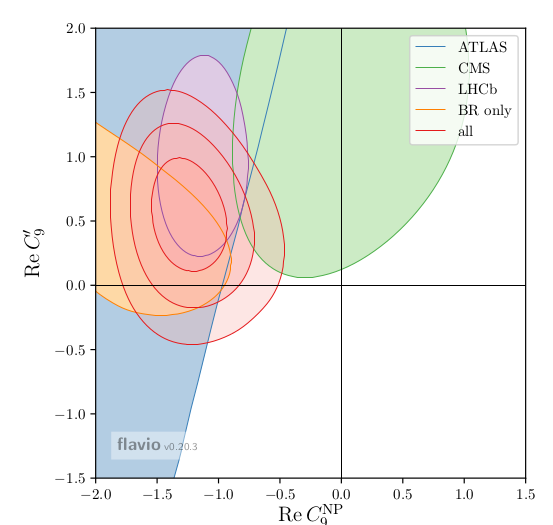
\includegraphics[width= \textwidth]{./assets/c9_c9} \\ $5.3\sigma$
		\end{center}	
	\end{columns}
%===========================================================
% Slide 14
%===========================================================
\end{frame}
\begin{frame}{Fits $ C^\mu$  VS $C^e$ }
	\begin{columns}[c]
		\column{.5\textwidth}
		\begin{center}
			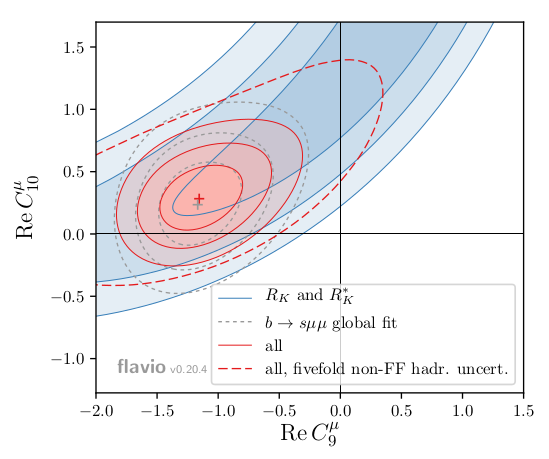
\includegraphics[width=0.7\textwidth]{./assets/c9_rk} \\ {\tiny$ C_0^\mu , C_{10}^\mu$}
		\end{center}
			\begin{center}
				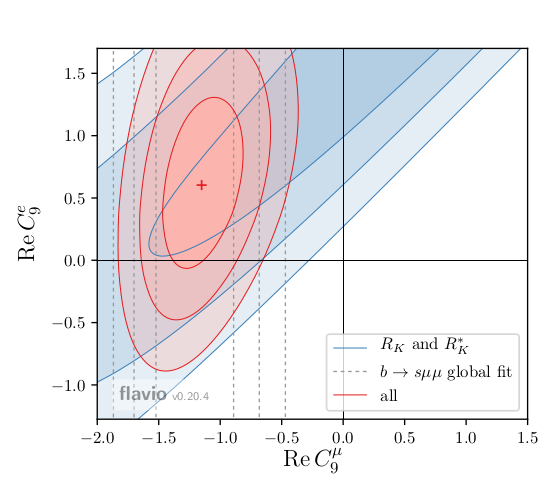
\includegraphics[width= 0.7\textwidth]{./assets/c9_mue} \\ {\tiny$ C_9^\mu , C_{9}^e$}
			\end{center}	
		\column{.5\textwidth}
		\begin{center}
			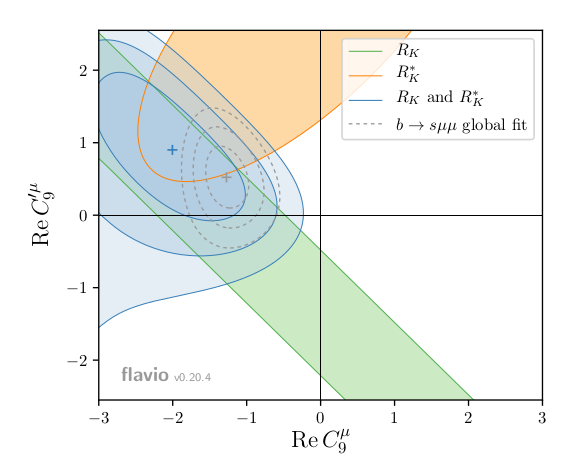
\includegraphics[width= \textwidth]{./assets/c9_c9p} \\ RH currents not favoured by data.. 
		\end{center}	
	\end{columns}
\end{frame}
%===========================================================
% Slide 15
%===========================================================
\begin{frame}{General scheme for NP Wilson coefficients  }
	\begin{columns}[c]
		\column{.6\textwidth}
		\begin{center}
			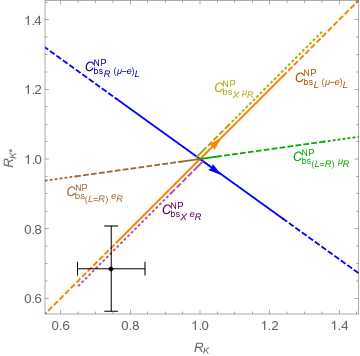
\includegraphics[width=0.8\textwidth]{./assets/RKRKs} \\{\tiny Carmona \& Goertz \arXivCode{1503.07138 }}  
		\end{center}
		\column{.4\textwidth}
		\begin{itemize}
			\item For LH chiral theories, electron currents does not not contribute;
			\item If  both RH and LH fermions couple to the NP we expect significant contribution from the electron.
		\end{itemize} 
	\end{columns}
\end{frame}
%\begin{frame}{Model independent fit for $\RD$}
%	\begin{columns}[c]
%		\column{.5\textwidth}
%		\begin{center}
%			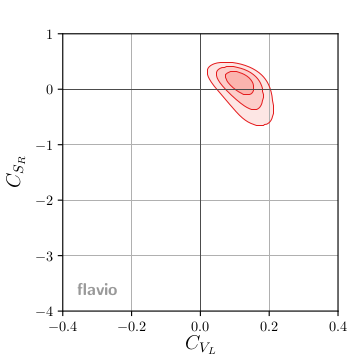
\includegraphics[width=0.7\textwidth]{./assets/cv_rd}
%		\end{center}
%		\begin{center}
%			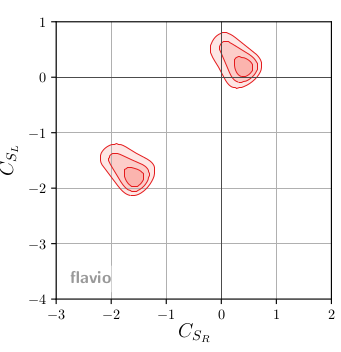
\includegraphics[width= 0.7\textwidth]{./assets/csr_rd} 
%		\end{center}	
%		\column{.5\textwidth}
%		\begin{center}
%			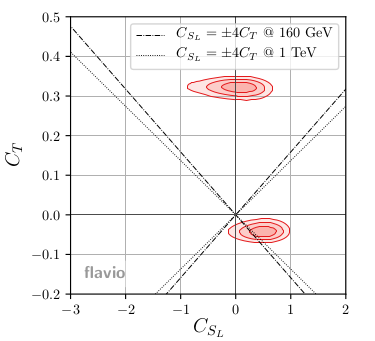
\includegraphics[width= 0.7\textwidth]{./assets/csl_rd} \\ data also favouers Left-handed Vector current contribution
%		\end{center}	
%	\end{columns}
%\end{frame}
%
%
%===========================================================
% Slide 16
%===========================================================
\begin{frame}{Summary }
	\begin{itemize}
		\item For the first time, we observe a consistent deviation from the SM from independently measured observables. \pause
		\item We need MORE DATA to eliminate the possibility of such tension coming from  statistical fluctuation. \pause
		\item Both $\RK$ and $\RD$ have about $\sim 25\%$ deviation from the SM.. \\ Any model explaining both is challenged by making NP  contribution for $b\to c\ell\nu$ be much larger than the FCNC of $ b \to s \ell \ell $. \pause
		\item The data favours vector currents coupled to LH fermions~ Chiral currents. \pause
		\item Any model needs to have contribution to $BR( B_s \to \mu \mu)$ with $ \approx 3\cdot 10^{-9}$.  \pause
		\item Typical models involve Leptoquarks with Pati-Salam-like Gauge structure.. $SU(4)\times SU(2)\times SU(2)$. \pause
		\item $Z^\prime$ or composite Higgs models are also viable candidates~(A. Carmona and F. Goertz). \pause
		\item  \alert{An observable similar to $\RK$ needs to be measured for $ B \to K \tau \tau$}.  
	\end{itemize}
\end{frame}
%===========================================================
% Slide 17
%===========================================================
\begin{frame}{The search for the decay $ B \to K^* \tau^+ \tau^-$ }
Extrapolating from $\RD$ anomalies, Capdevila \textit{et al }~\arXivCode{1712.01919} predicted enhancement of the BR with $\tau$'s up to $10^3$
	\begin{center}
		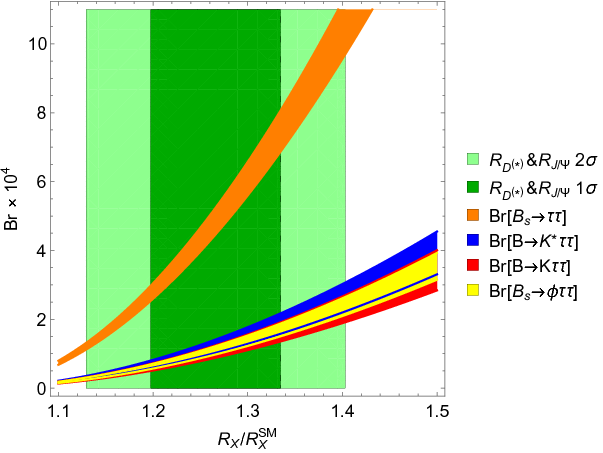
\includegraphics[width= 0.6\textwidth]{./assets/RX} 
	\end{center}
	\pause
	We expect enhancement of $\sim 10^{+3}$ of the SM for $ B \to K^* \tau^+ \tau^-$ BR..
\end{frame}
%===========================================================
% Slide 18
%===========================================================
\begin{frame}{The search for the decay $ B \to K^* \tau^+ \tau^-$ }
Nevertheless, the search for this decay is challenging due to its complex topology, particularly in hadronic machines... 
	\begin{columns}[c]
		\column{.5\textwidth}
		\begin{center}
		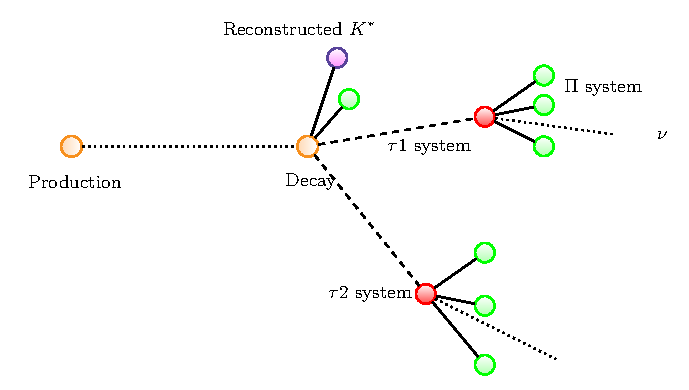
\includegraphics[width= \textwidth]{./assets/topology1}
		\end{center}
		\column{.5\textwidth}
		\begin{center}
		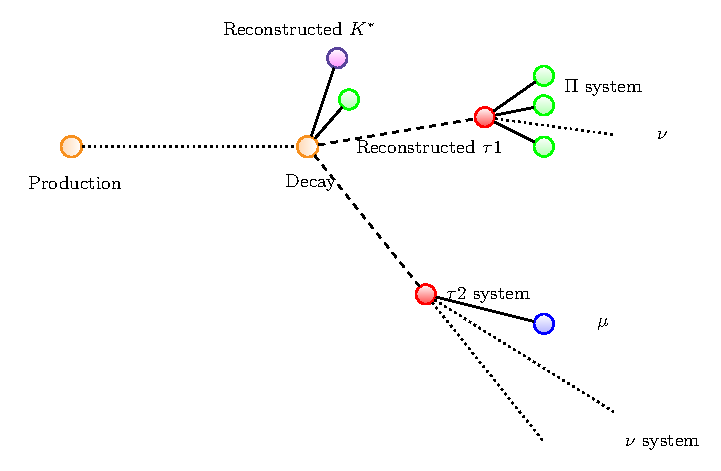
\includegraphics[width= \textwidth]{./assets/topology2}
			\end{center}
	\end{columns}
\pause
Considering both $\tau$ final states we could reconstruct $\sim 5 \%$ of these decays.. 
\end{frame}
%
%\begin{frame}{Reconstruction technique }
%\begin{itemize}
%	\item It is possible to obtain an exact solution for the 3 prong $\tau$ final state $ \tau \to 3 \pi$, this is not the case for $ \tau \to \mu \nu \bar \nu$. \pause 
%	\item However, combinatorics, both giving a factor of 4. \pause
%	\item A solution for the topological reconstruction for the decays type $ 3\pi \mu$ can be written as a function of the di-neutrino effective mass:
%	\begin{equation}
%	m_N = \sqrt{2p_{\nu} p_{\bar \nu}(1- \cos \theta_{\nu \bar \nu})}
%	\end{equation} \pause
%	\item The correlation between this unmeasurable quantity and the perpendicular component   of the muon momentum w.r.t. the B direction can be established and hence improving the solution empiricaly. 
%\end{itemize}
%\end{frame}
%
%===========================================================
% Slide 19
%===========================================================
\begin{frame}{The effective di-neutrino mass }
	\begin{columns}[c]
		\column{.5\textwidth}
	The internal degrees of freedom for the 2 neutrinos in the $ \tau \to \mu \nu \bar \nu$ cannot be constraint from the decay topology, using the TRUTH MC we can plot the distribution for this parameter:
		\begin{equation}
		m_N = \sqrt{2p_{\nu} p_{\bar \nu}(1- \cos \theta_{\nu \bar \nu})}\nonumber
		\label{MN}
		\end{equation}
		\column{.5\textwidth}
		\begin{center}
			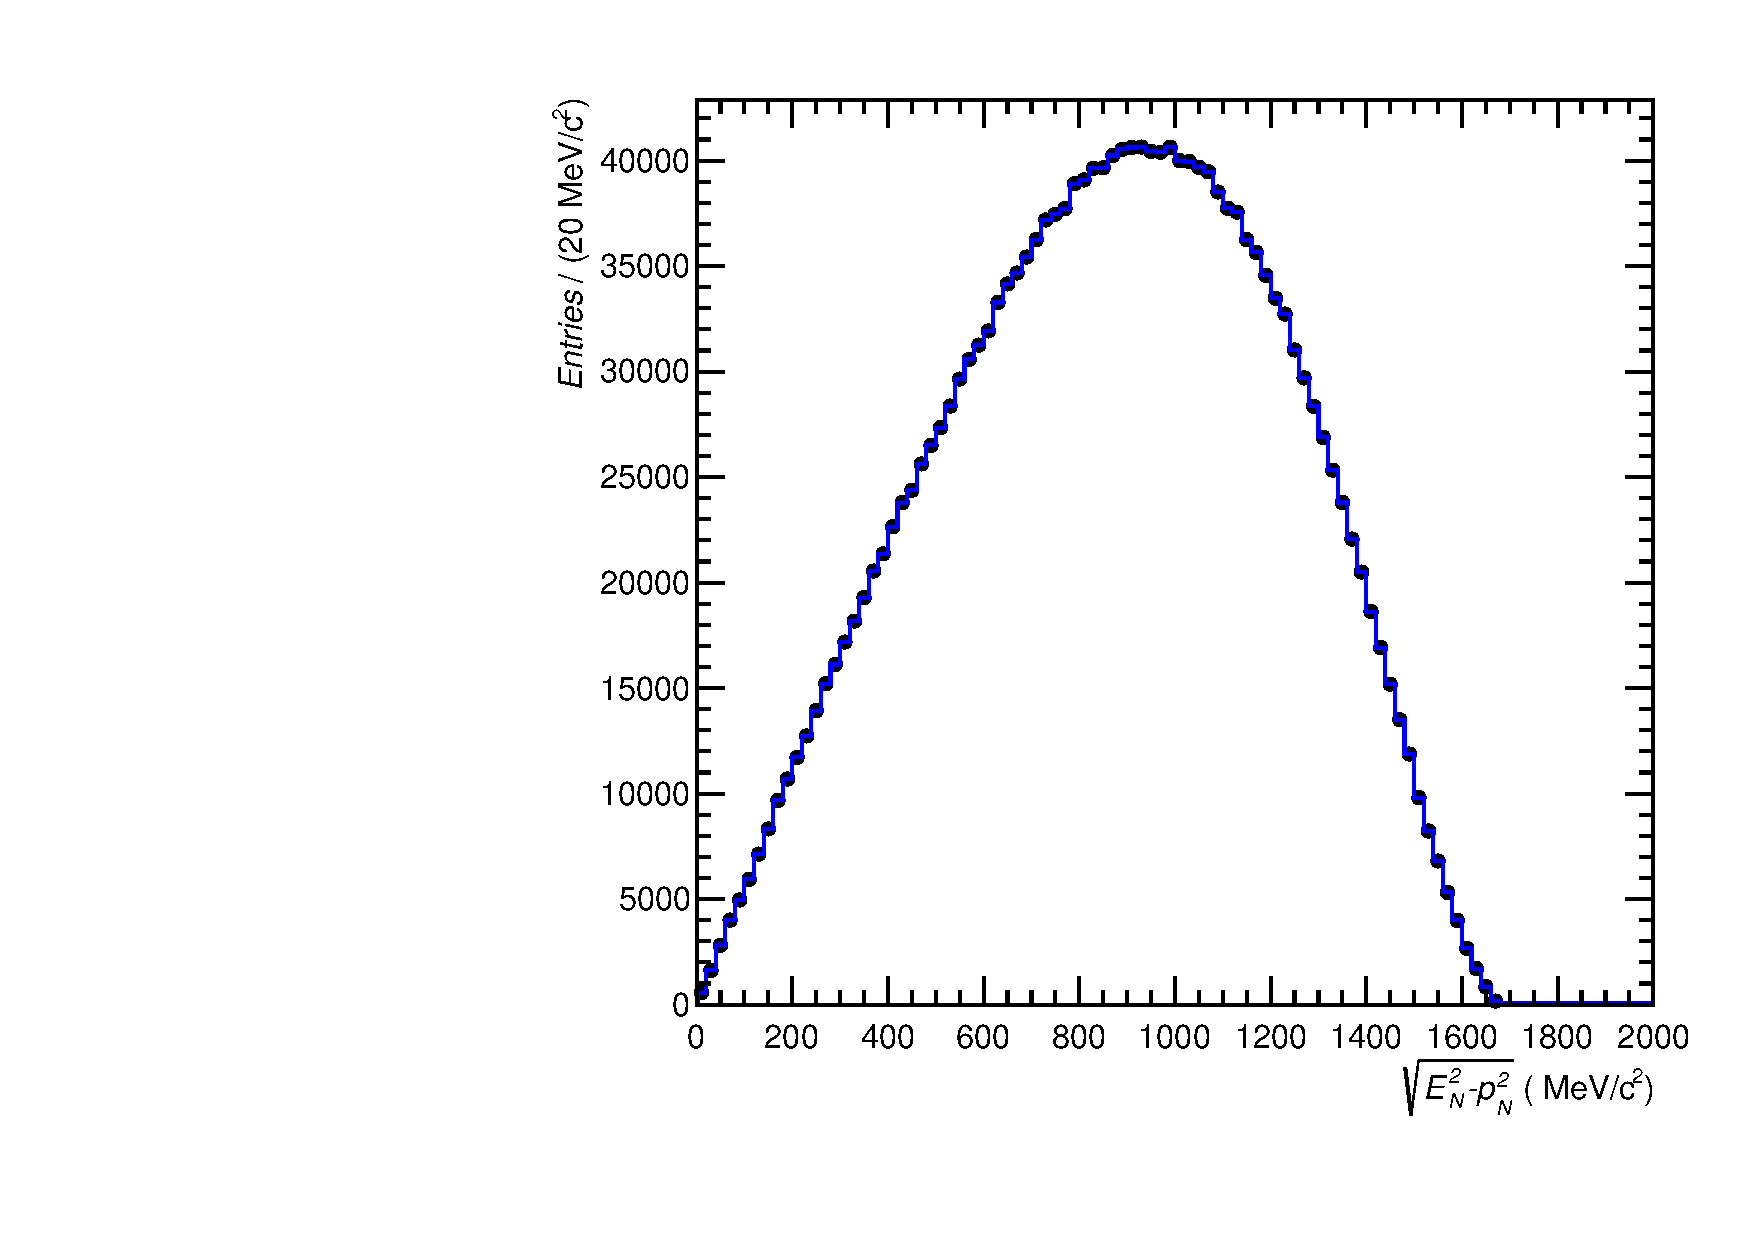
\includegraphics[width= \textwidth]{./assets/can_meff_3pimu_FullTRUE_0.pdf} 
		\end{center}
	\end{columns}
\end{frame}
%===========================================================
% Slide 20
%===========================================================
 \begin{frame}{Testing the solution of TRUTH sample}
The reconstruction equations using the mean of  $m_N$ as a fixed value was tested on TRUTH MC:
 	\begin{center}
 		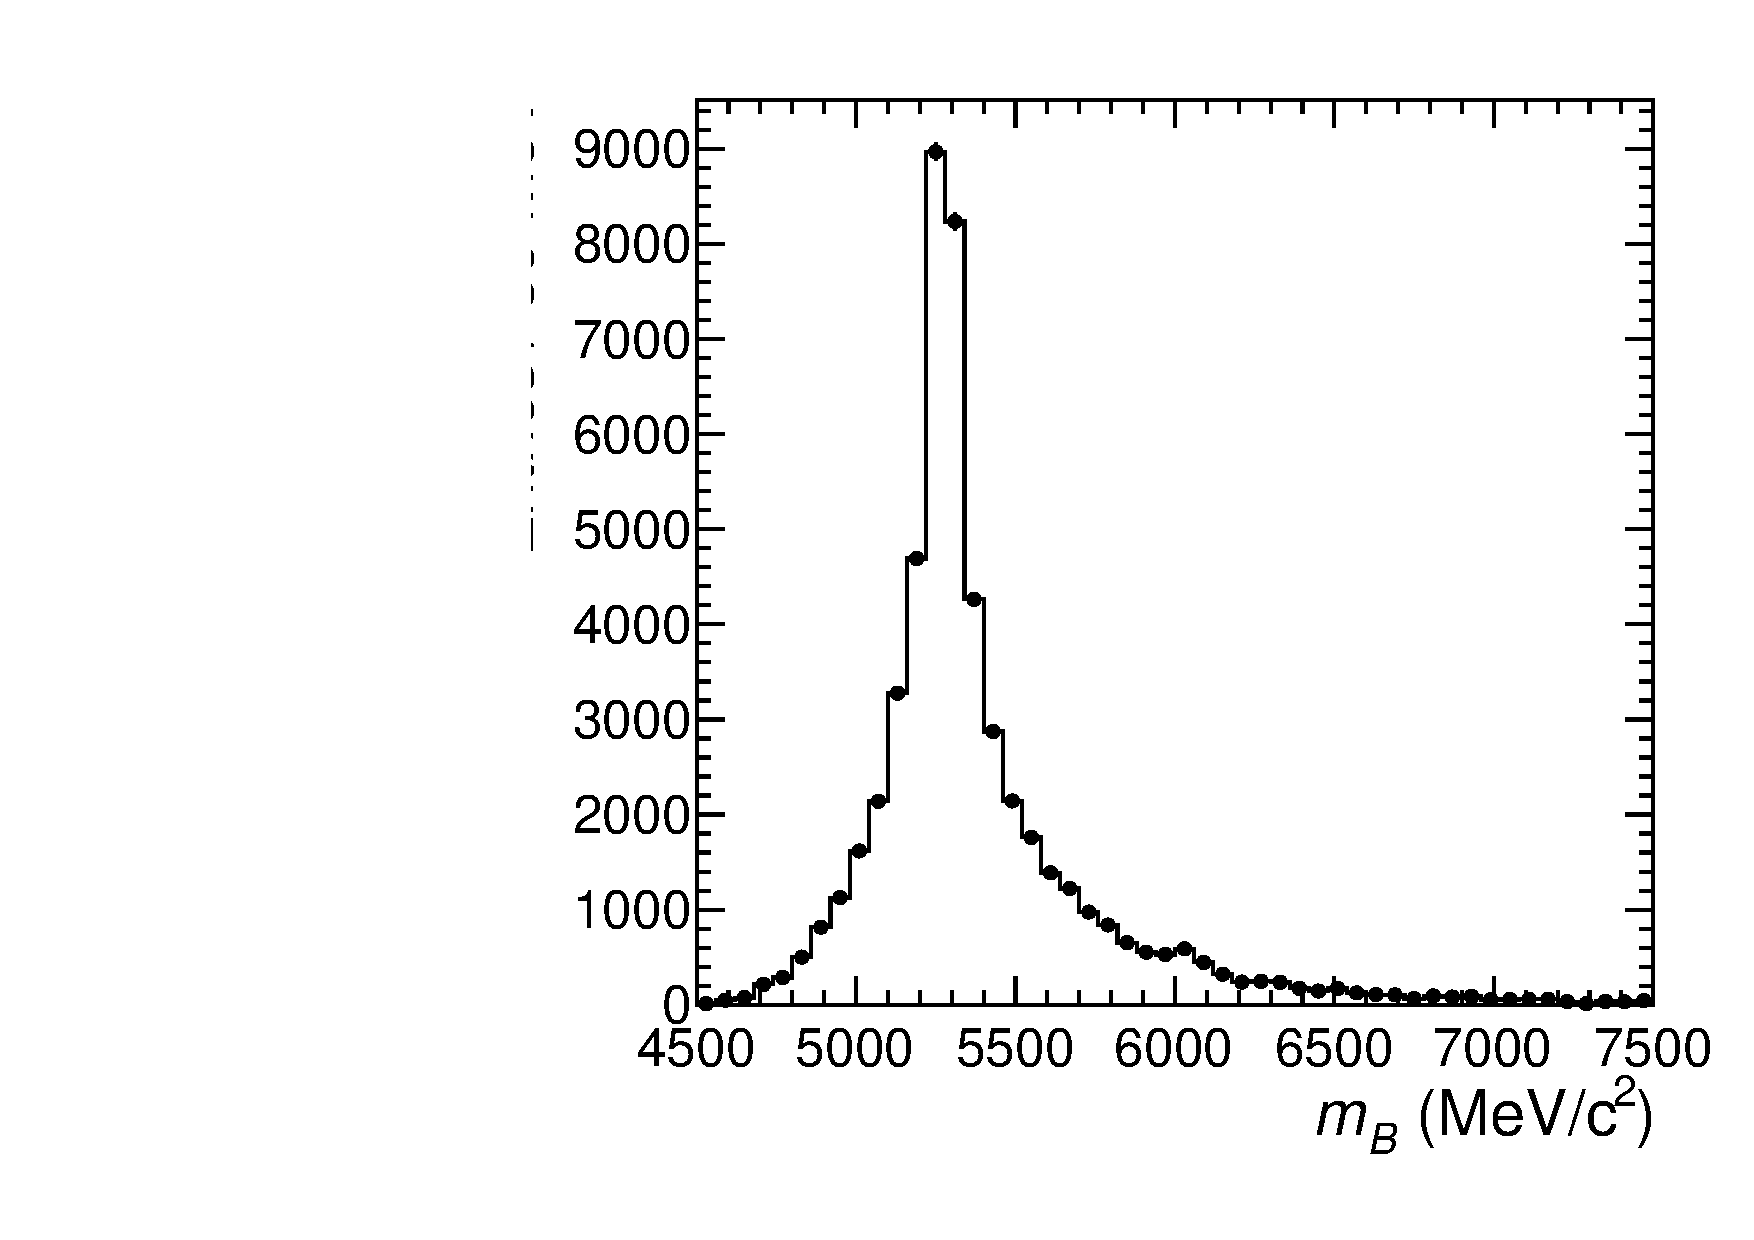
\includegraphics[width=.55\textwidth]{assets/Distribution_Bmass_RR_3pimu_FullTRUE}
 	\end{center}
 \end{frame}
%===========================================================
% Slide 21
%===========================================================
\begin{frame}{ Search for correlation}
	\begin{columns}[c]
		\column{.5\textwidth}
		
		A 2-D histogram between~$ p_\mu^\bot$ and~ $m_N$ was constructed from TRUTH events to study the possibility of correlating the 2 variables, as seen in the figure, possible anti-correlation is observed. The correlation factor is found to be~$r=-0.503$.
		
		\column{.5\textwidth}
		\begin{center}
			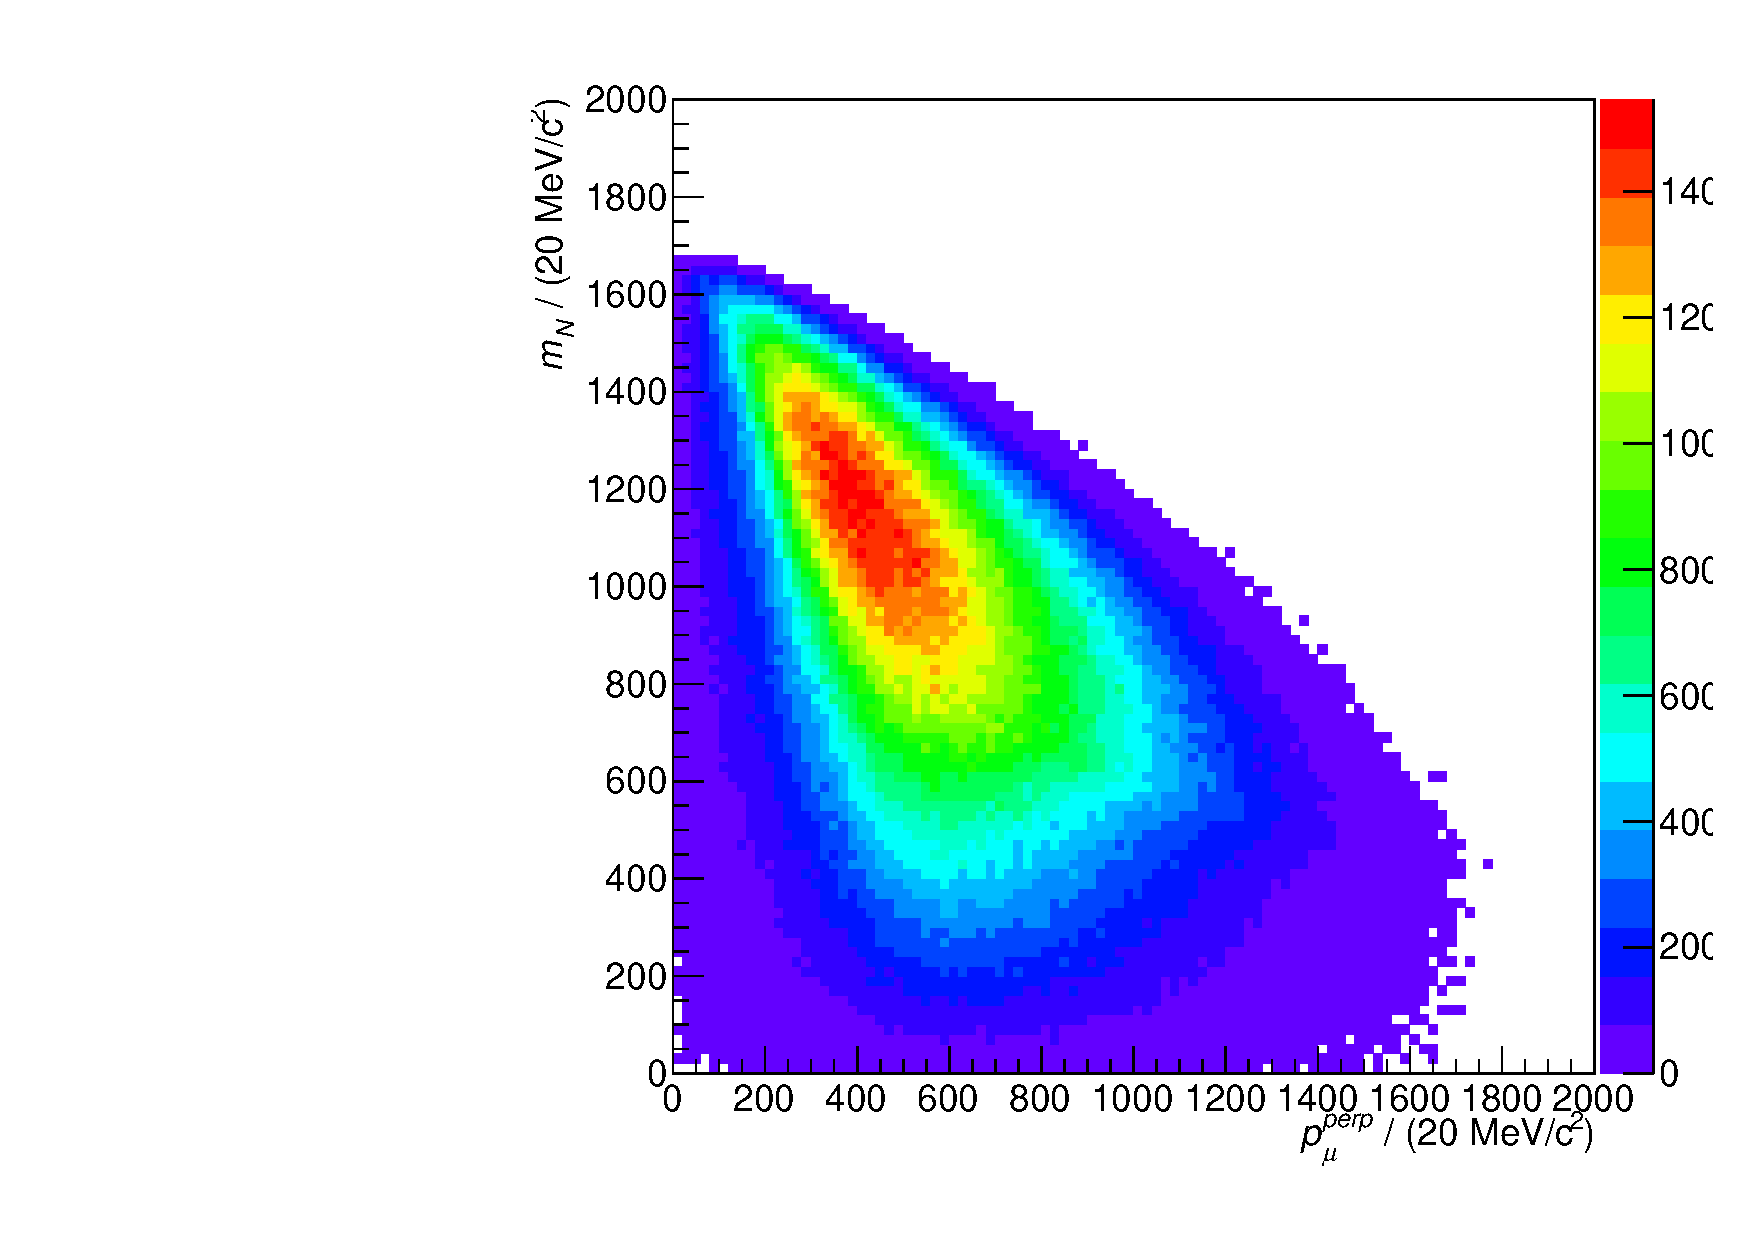
\includegraphics[width= \textwidth]{./assets/pmu_perp} 
		\end{center}
	\end{columns}
	The correlation is stronger for low~$ p_\mu^\bot$ events. While for the large $ p_\mu^\bot$ values it is less prominent. 
\end{frame}

%\begin{frame}{linear model}
%	Since a moderate anti-correlation between~$p_\mu ^\bot$ and $m_N$ was found, a linear model for them was constructed from fitting their 2-D histogram. 
%	\begin{table}
%		\centering
%		\begin{tabular}{l c c }
%			\hline
%			parameter & value & uncertainty ($\pm$) \\
%			\hline
%			$p_1 $& $-0.59$ & $0.03$\\
%			$p_0 $& $1318.69$ & $15.38$\\
%			\hline
%		\end{tabular}
%	\end{table}
%	Hence the effective mass $ m_N$ in the solution will be substituted with its linear model: 
%	\begin{equation}
%	m_N = -0.59 p_\mu^\bot + 1318.69
%	\end{equation}
%\end{frame}
%%===========================================================
%% Slide 22
%%===========================================================
\begin{frame}{Testing the solution with linear model on TRUTH}
	The solution with the linear model for $m_N$ was tested on TRUTH simulation, and the left-tail of the B-mass histogram was fit by a Gaussian :
	\begin{columns}[c]
		\column{.5\textwidth}
		\begin{table}
			\centering
			\begin{tabular}{l  c c }
				\hline
				& value (MeV) & Err ($\pm$ MeV) \\
				\hline
				mean & $5306.26$  & $68.71$  \\
				RMS & $147.72$ & $84.78$ \\
				\hline
			\end{tabular}		
		\end{table}
		\column{.5\textwidth}
		\begin{center}
			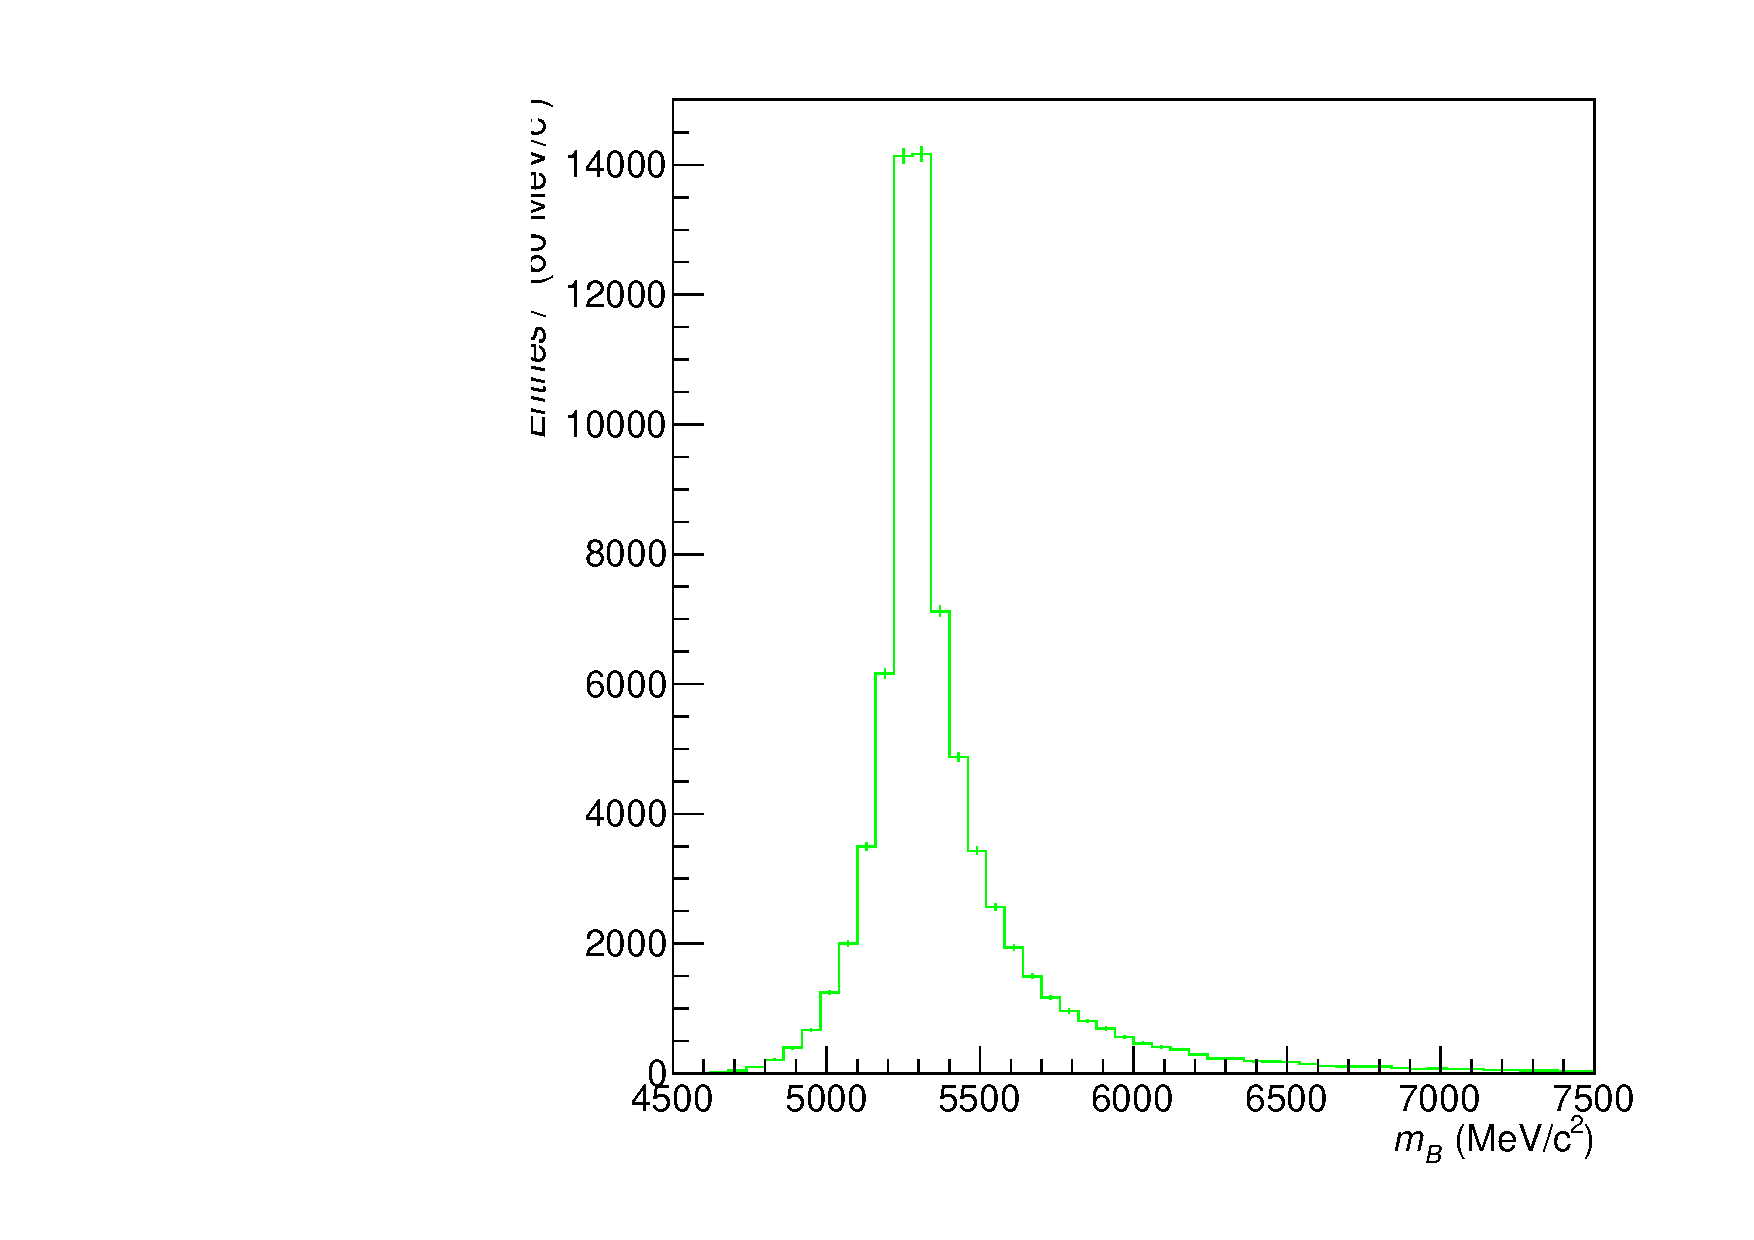
\includegraphics[width= \textwidth]{./assets/linear_model_3pimu} 
		\end{center}
	\end{columns}
\end{frame}
%%===========================================================
%% Slide 23
%%===========================================================
\begin{frame}{Testing the solution with linear model on TRUTH}

	\begin{columns}[c]
		\column{.5\textwidth}
\begin{center}
	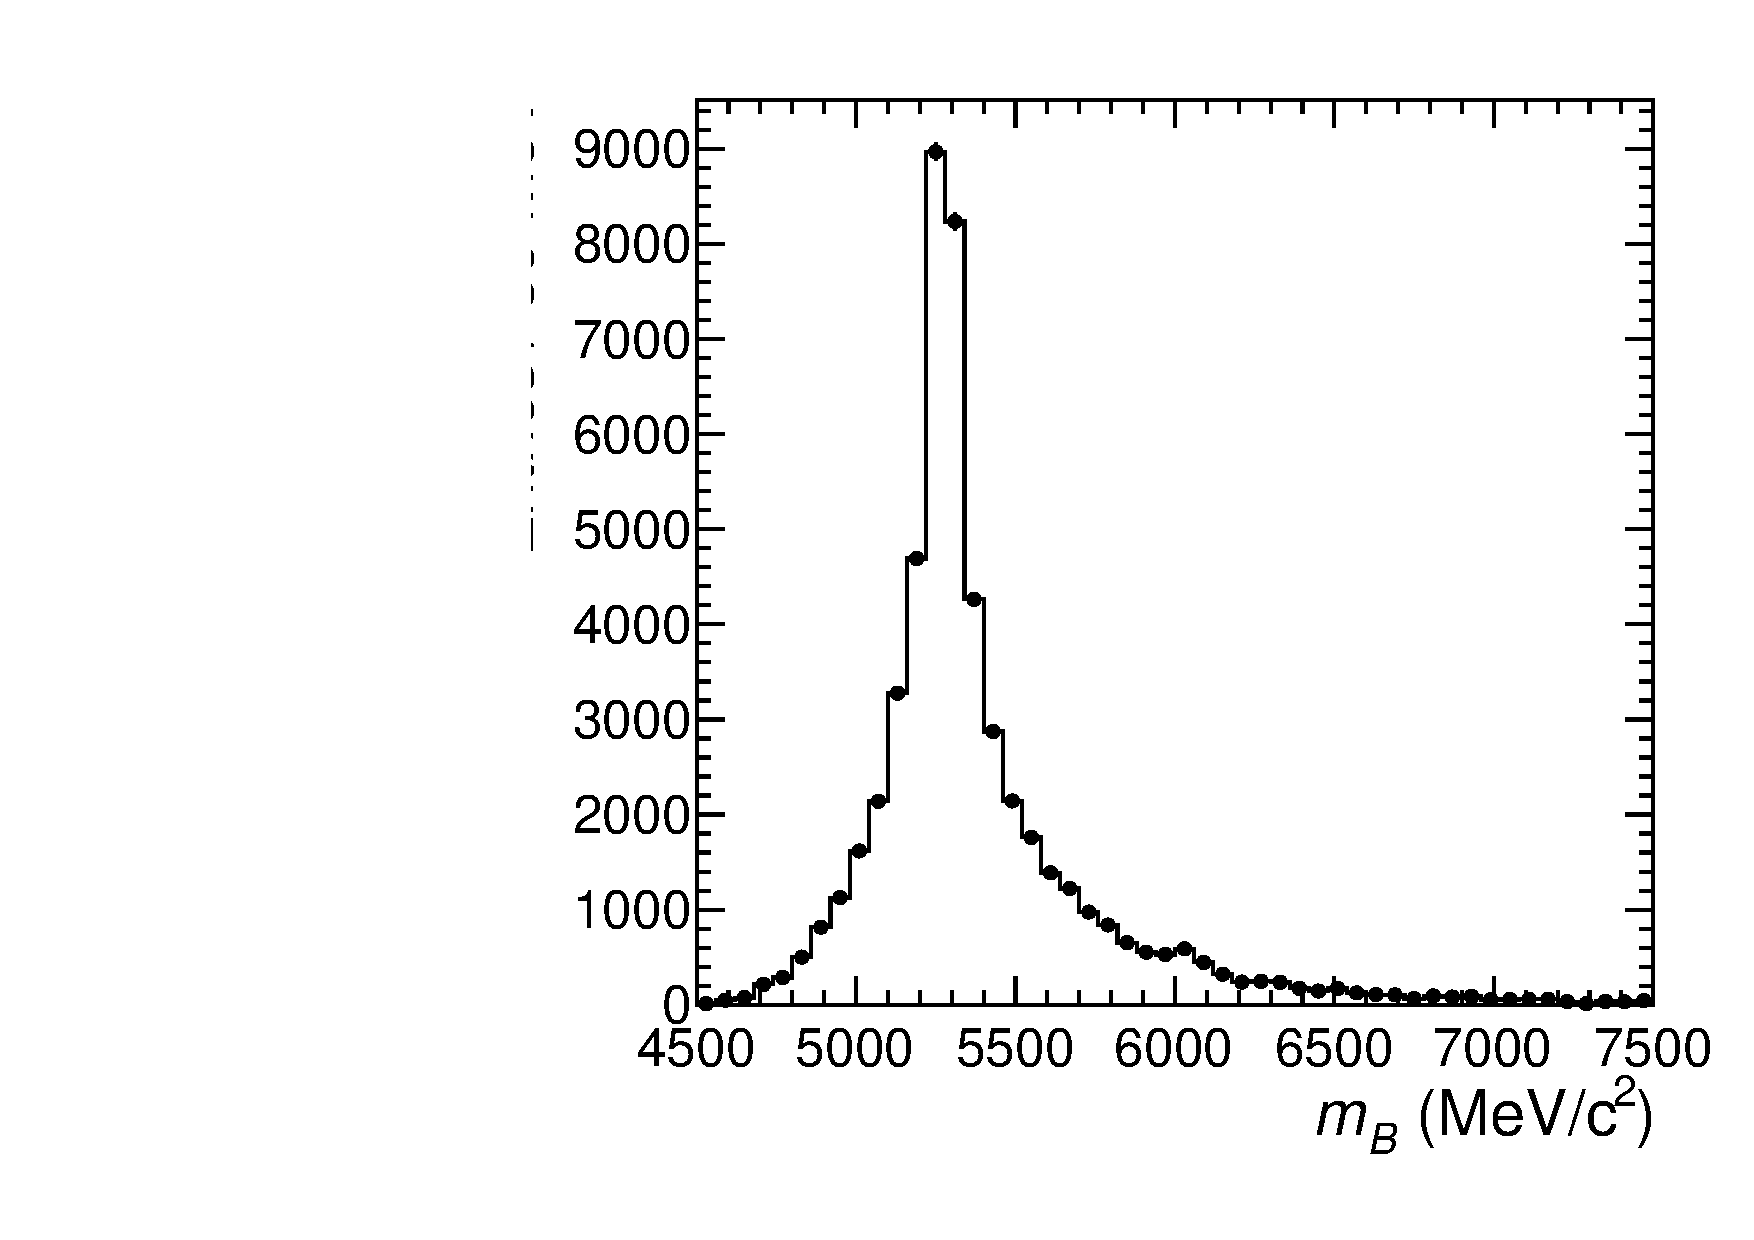
\includegraphics[width=\textwidth]{assets/Distribution_Bmass_RR_3pimu_FullTRUE}
\\ before
\end{center}
		\column{.5\textwidth}
		
		\begin{center}
	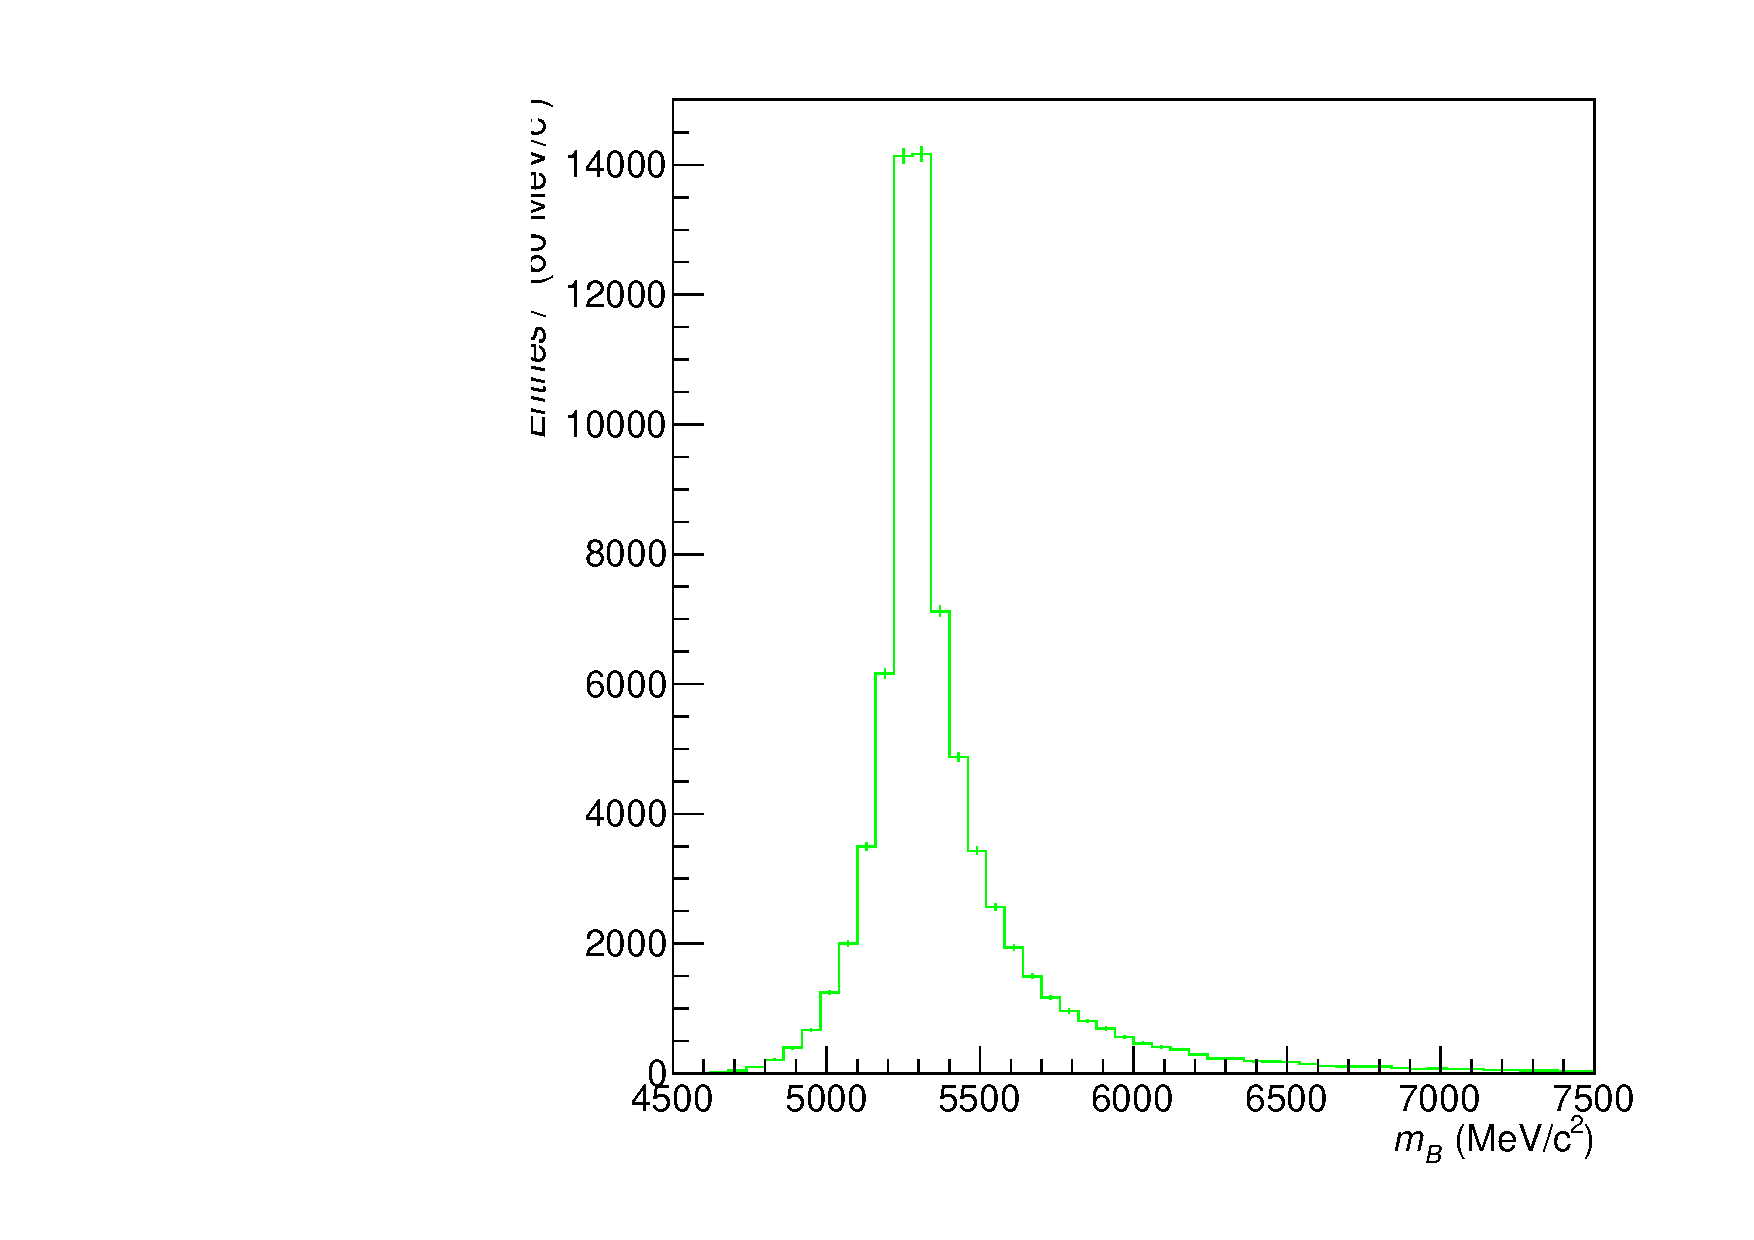
\includegraphics[width= \textwidth]{./assets/linear_model_3pimu} 
	\\after
		\end{center}
	\end{columns}
\end{frame}
%%===========================================================
%% Slide 24
%%===========================================================
\begin{frame}{Testing the solution with linear model on REC}
	The solution with the linear model for $m_N$ was tested on REC simulation, and the left-tail of the B-mass histogram was fit by a Gaussian :
	\begin{columns}[c]
		\column{.5\textwidth}
		\begin{table}
			\centering
			\begin{tabular}{l  c c }
				\hline
				& value (MeV) & Err ($\pm$ MeV) \\
				\hline
				mean & $5381.28$  & $95.05$  \\
				RMS & $282.92$ & $63.75$ \\
				\hline
			\end{tabular}
		\end{table}
		\column{.5\textwidth}
		\begin{center}
			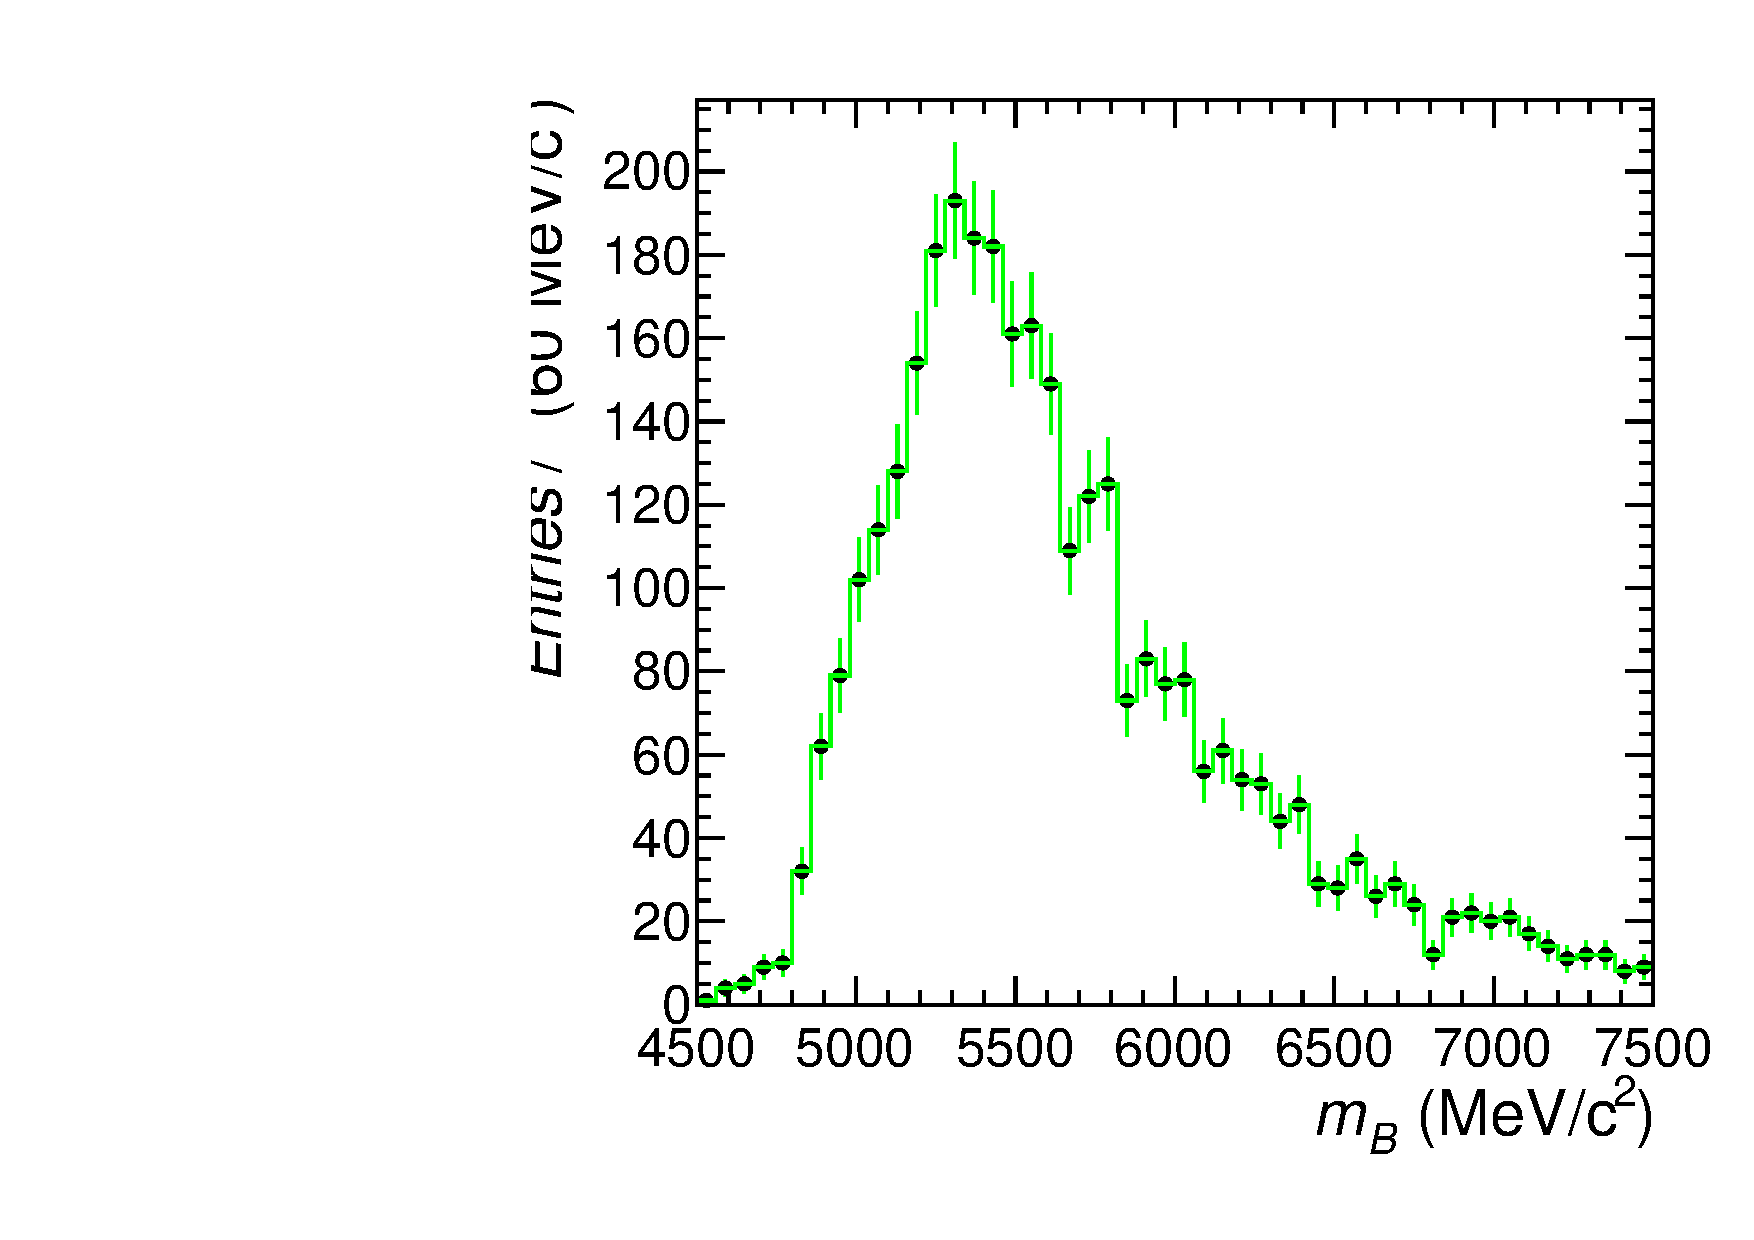
\includegraphics[width= \textwidth]{./assets/linear_model_reco} 
		\end{center}
	\end{columns}
\end{frame}
%%===========================================================
%% Slide 25
%%===========================================================
\begin{frame}{Efficiency evaluation}
	The reconstructibility and stripping efficiencies $\varepsilon_{\text{Rec}}\cdot\varepsilon_{\text{Strip}}= N_{REC}/N_{TRUTH}$  of the 3pi 3pi and 3pimu decays are
	\begin{table}[!htbp]	
		\centering
		\begin{tabular}{l  c c }
			\hline
			Decay mode & $\varepsilon_{\text{Rec}}\cdot \varepsilon_{\text{Strip}} (\%)$ & uncertainty $\pm (\%)$  (95\% CL)\\
			\hline
			3pi3pi & $0.86$ & $ 0.07$ \\
			3pimu & $ 0.03$& $ 0.04$ \\
			\hline
		\end{tabular}
		\label{eta_rec}
	\end{table}
	Moreover, the reconstruction method efficiencies for both decays are
	\begin{table}
		\label{eta_meth}
		\centering
		\begin{tabular}{l  c c }
			\hline
			Decay mode & $\varepsilon_{\text{Meth}} (\%)$ &  uncertainty$\pm (\%)$ (95\% CL)\\
			\hline
			3pi3pi & $18.20$ & $ 0.41$ \\
			3pimu & $ 19.86$& $ 0.46$ \\
			\hline
		\end{tabular}
	\end{table}
\end{frame}
%\begin{frame}{Conclusions}
%	\begin{itemize}
%		\item There is a moderate correlation between the $B$--perp muon momentum~$p_\mu^\bot$ and the di-neutrino effective mass~$m_N$, that can be utilised for constructing an empirical model linking the two together. 
%		\item This model can be used in the solution for the invariant B-mass to substitute the unmeasurable $m_N$ with a the measurable quantity $p_\mu^\bot$. 
%		\item A linear model seems to be suitable, in particular for low $p_\mu^\bot$ values. For large $p_\mu^\bot$ events, it is difficult to establish a correlation with $m_N$. 
%		\item Using the linear model improved the solution, as can be seen from the invariant B-mass histograms, the bin with most events is indeed the real B-mass bin.
%		\item A contiuation for this work would be by: Studying higher order models for $p_\mu^\bot$ and $m_N$, that could include the large $p_\mu^\bot$ events. \\ Test the model against backgrounds.
%	\end{itemize}
%\end{frame}

%%===========================================================
%% Slide 26
%%===========================================================
\begin{frame}{ SU(2)\times U(1) LQ Model}
New vector Leptoquark is based on extending the SM symmetry by a group similar to the EW group, i.e.
\[   \mathrm{pre\;GUT} \longrightarrow SU(3)_c \times SU(2)_{\text{LQ}} \times SU(2)_{\mathrm{W}} \times U(1)_{X} \longrightarrow  SU(3)_c \times SU(2)_{\mathrm{W}} \times U(1)_{Y} \] \pause
\begin{itemize}
	\item The model is chiral, coupling only to left-handed currents. \pause
	\item  Introducing an $SU(2)$ triplet $ V^a_\mu$ and a $U(1)$ $C_\mu$ gauge bosons with coupling constants $ g_{\mathrm{LQ}}$ and  $g'_{\mathrm{LQ}}$, respectively.
	\item After the SSB, three bosons acquire mass and one is left massless we identify as the $B_\mu$ boson associated with the weak hypercharge $Y$. \pause
	\item The scale of the SSB of this model is expected to be $\Lambda_{\mathrm{LQ}}\sim$~\TeV. 
\end{itemize}
\end{frame}
%%===========================================================
%% Slide 27
%%===========================================================
\begin{frame}{The Model}
	There is an immediate constraint on this model for the mixing angle of $ V^3_\mu$ and~$ C_\mu$ from the weak mixing angle and the EM fine structure constant, at $\Lambda_{EW}$:
	\begin{columns}[c]
		\column{.5\textwidth}
		\begin{center}
			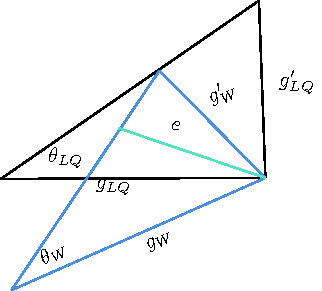
\includegraphics[width= 0.5\textwidth]{./assets/triangles} 
		\end{center}
		\column{.5\textwidth}
		\[( g'_{\mathrm{LQ}})^2=4 \pi \alpha_{\mathrm{EM}}\; \frac{1}{\cos^2\theta_W \sin^2\theta_{LQ}} \]	
	\end{columns}
	For natural $ g'_{\mathrm{LQ}}$, one expects $ \theta_{\mathrm{LQ}} \approx 18.65$ deg. \\ Implying that $M_U = 1.05 \, M_V$
\end{frame}
%%
%%
%\begin{frame}{The Lagrangian}
%	The total Lagrangian of this model with the Standard model is given by:
%	\[\mathcal L = \mathcal{L}_{\mathrm{QCD}}+\mathcal{L}_{\mathrm{EW}}+\mathcal{L}_{\mathrm{LQ}}+\mathcal{L}_{\phi}+\mathcal{L}_{h}+ \mathcal{L}_{\mathrm{f\,kin}}. \]
%	Where:
%	\begin{align*}
%		\mathcal{L}_{\mathrm{QCD}}\;& \Longrightarrow \;\text{QCD Lagragian} \\ 
%		\mathcal{L}_{\mathrm{EW}}\;& \Longrightarrow \;\text{EW Lagragian, without the B feild}\\
%		\mathcal{L}_{\mathrm{LQ}}\;& \Longrightarrow \;\text{LQ Lagragian,}\;\SUgroup{2}\times \Ugroup{1}\\
%		\mathcal{L}_{\phi}\;& \Longrightarrow \;\text{new complex  scalar doublet, causing SSB-1 at }\, \Lambda_{LQ}\\
%		\mathcal{L}_{h}\;& \Longrightarrow \;\text{BEH field, causing SSB-2 at }\, \Lambda_{EW}\\
%		\mathcal{L}_{\mathrm{f\,kin}}\;& \Longrightarrow \;\text{kinetic term for fermions}
%	\end{align*}
%\end{frame}
%%===========================================================
%% Slide 28
%%===========================================================
\begin{frame}{The Lagrangian}
	The gauge leptoquark lagrangian is given by:\
	\begin{align*}
		\mathcal{L}_{\mathrm{LQ}} =& -\frac{1}{4}\parenths{ V_{\mu \nu}^aV^{\mu \nu}_a + C_{\mu\nu}C^{\mu\nu}}-ig_{LQ}\sqbracs{\bar{LQ}_{U_L} \frac{\sigma ^a}{2} \slashed{V}_a  LQ_{U_L}}\\				\qquad& -ig_{LQ}\sqbracs{\bar{LQ}_{D_L} \frac{\sigma ^a}{2} \slashed{V}_a   LQ_{D_L}} -ig'_{LQ}\sqbracs{\bar{LQ}_{U(D)_L} (IX) \slashed{C}  LQ_{U(D)_L}} \\ \qquad& -ig'_{LQ}X\sqbracs{\bar{U(D)}_R \slashed{C}U(D)_R+\bar{E}_R \slashed{C} E_R}.
	\end{align*}
	With:
	\begin{align*}
		LQ_{U_L} := \braces{ \textcolor{red}{\colvector{u_L \\ \nu_e}};\colvector{c_L \\ \nu_\mu} \; ; \colvector{t_L \\ \nu_\tau} },\; 
		LQ_{D_L} := \braces{ \textcolor{red}{\colvector{d_L \\ e_L}};\colvector{s_L \\ \mu_L} \; ; \colvector{b_L \\ \tau_L} }, \\ 
		U_R:= \braces{\textcolor{red}{u_R}, c_R,t_R}, \;  D_R:= \braces{\textcolor{red}{d_R}, s_R,b_R} ,\; E_R:= \braces{\textcolor{red}{e_R}, \mu_R,\tau_R}.
	\end{align*}
	The first family - in red- does not couple to the leptoquarks
\end{frame}
%\begin{frame}{Spontaneous Symmetry breaking}
%	There are 2 SSB stages :
%	\begin{columns}[c]
%		\column{.5\textwidth}
%		\begin{block}{LQ SSB}
%			\begin{tiny}
%				The $V$ bosons acquire a mass $M_V$ and we have the following physical states:
%				\begin{align*} 
%					&V^{\pm}_\mu = \frac{1}{\sqrt{2}}\parenths{V^1_\mu \mp i V^2_\mu}& U_\mu = -\sin \theta_{LQ} C_\mu + \cos \theta_{LQ} V^3_\mu \\
%					& B_\mu = \cos \theta_{LQ} + \sin \theta_{LQ} V^3_\mu  & M_U = \frac{M_V}{\cos \theta_{LQ}}. \\
%					&  X \to Y  & M_V = \frac{v_\phi |g_{LQ}|}{2}.
%				\end{align*}
%			\end{tiny}
%		\end{block}
%		\column{.5\textwidth}
%		\begin{block}{EW SSB}
%			\begin{tiny}
%				The $W$ bosons acquire a mass $M_W$ and we have the following physical states:
%				\begin{align*} 
%					&W^{\pm}_\mu = \frac{1}{\sqrt{2}}\parenths{W^1_\mu \mp i W^2_\mu}& Z_\mu = -\sin \theta_{W} B_\mu + \cos \theta_{W} W^3_\mu \\
%					& A_\mu = \cos \theta_{W} + \sin \theta_{W} W^3_\mu  & M_Z = \frac{M_W}{\cos \theta_{W}}. \\
%					&  Y \to Q_e  & M_W = \frac{v_h |g_{W}|}{2}.
%				\end{align*}
%			\end{tiny}
%		\end{block}
%	\end{columns}
%	
%	
%	%Then the Electroweak SSB occurs .  Giving quarks and charged leptons masses and allow for flavour mixing.
%\end{frame}
%\begin{frame}{Quark-Lepton complementarity }
%The flavour mixing of quarks and leptons is expressed in the~$\mathcal V_{CKM}$ and $ \mathcal V_{PMNS}$ matrices. The quark-lepton complementarity requires a correlation matrix $\mathcal V_M$, that the LQ model can describe its shape:
%\[ \mathcal V_M = \mathcal V_{CKM} \cdot\mathcal  V_{PMNS} = \mathcal U^u_{LQ} \mathcal U^d_{LQ}\,^\dagger \]
%Where $ \mathcal U^u_{LQ}  $ and $\mathcal U^d_{LQ}$ are the leptoquark flavour  mixing matrices that emerge naturally from the flavour mixing in the SM. \\ One can impose bimaximal mixing for $\mathcal V_M$, heavily suppressing the 1st generation from appearing in the LQ, with renormalization. \\ This however, is constraint a lot and need further investigation, for example only works with quasi-degenerate neutrino masses.
%\end{frame}
%%
%%
%%===========================================================
%% Slide 29
%%===========================================================
\begin{frame}{Flavour mixing }
	The  LQ flavour mixing matrices are given by
	\[ \mathcal U^u_{LQ}=
	\begin{pmatrix}
	\textcolor{red}{\mathcal U_{u\nu_e}} & \textcolor{red}{\mathcal U_{u\nu_\mu}} & \textcolor{red}{\mathcal U_{u\nu_\tau} } \\
	\textcolor{red}{\mathcal U_{c\nu_e}} & \textcolor{green}{\mathcal U_{c\nu_\mu}} &  \textcolor{blue}{\mathcal U_{c\nu_\tau}}\\
	\textcolor{red}{\mathcal U_{t\nu_e}} & \textcolor{blue}{\mathcal U_{t\nu_\mu}} &  \textcolor{green}{\mathcal U_{t\nu_\tau}}
	\end{pmatrix}
	\] 
	\[ \mathcal U^d_{LQ}=
	\begin{pmatrix}
	\textcolor{red}{\mathcal U_{d e}} & \textcolor{red}{\mathcal U_{d \mu}} & \textcolor{red}{\mathcal U_{d \tau} } \\
	\textcolor{red}{\mathcal U_{s e}} & \textcolor{green}{\mathcal U_{s\mu}} &  \textcolor{blue}{\mathcal U_{s\tau}}\\
	\textcolor{red}{\mathcal U_{be}} & \textcolor{blue}{\mathcal U_{b\mu}} &  \textcolor{green}{\mathcal U_{b\tau}}
	\end{pmatrix}
	\] 
	Where the terms in \textcolor{green}{green} are the largest, in \textcolor{blue}{blue} are smaller, and the ones in \textcolor{red}{red} are of $ \sim \lambda^4$ or less. \\
	\begin{center}
		\[\lambda \sim \mathcal O(10^{-1}) \]
	\end{center}
	The exact determination of the values of such mixings need to be determined from experimental fits..
\end{frame}
%%===========================================================
%% Slide 30
%%===========================================================
\begin{frame}{Feynman Rules }
	There are charged and neutral currents:
	\begin{columns}[c]
		\column{.5\textwidth}
		\begin{center}
			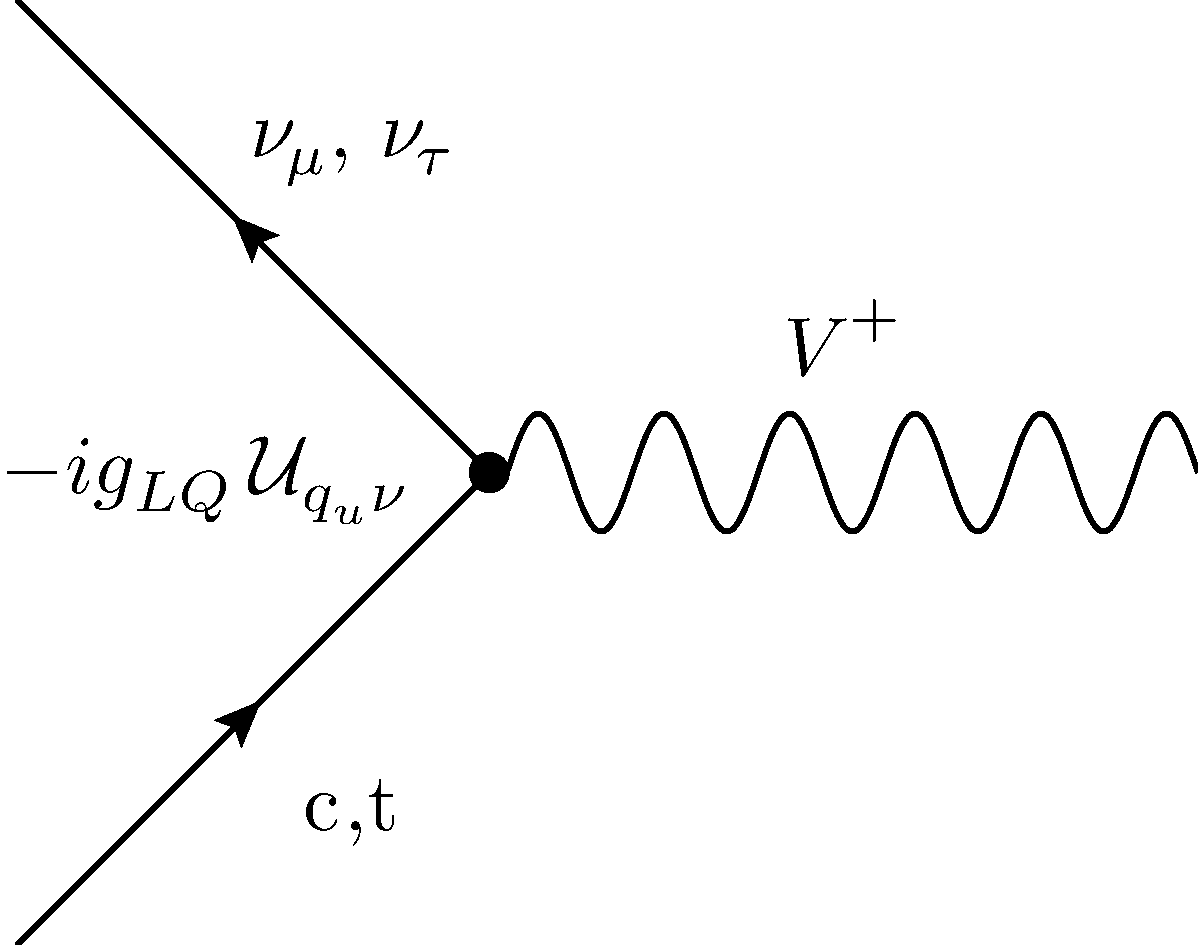
\includegraphics[width= 0.5\textwidth]{./assets/charged_current} \\
			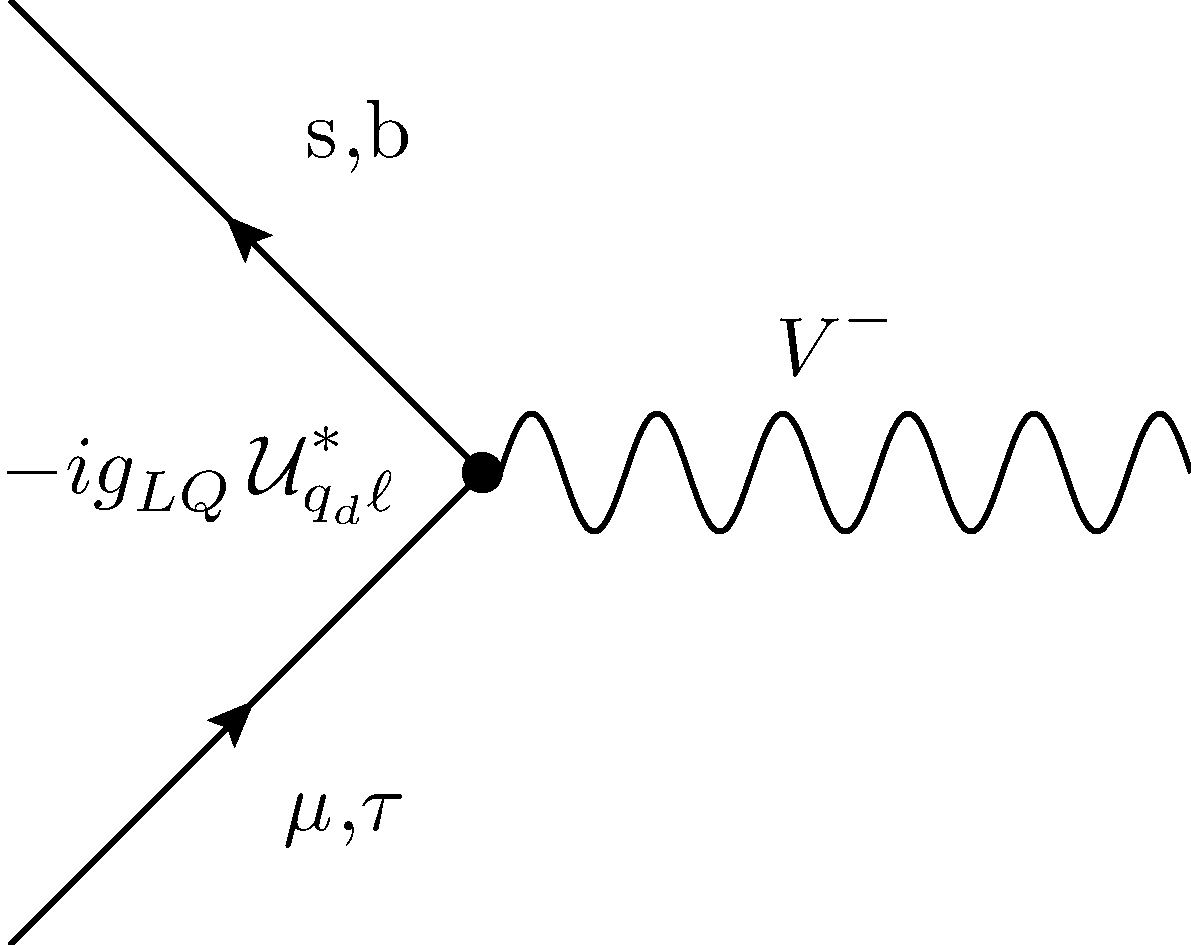
\includegraphics[width= 0.5\textwidth]{./assets/charged_current2} 
		\end{center}
		\column{.5\textwidth}
		\begin{center}
			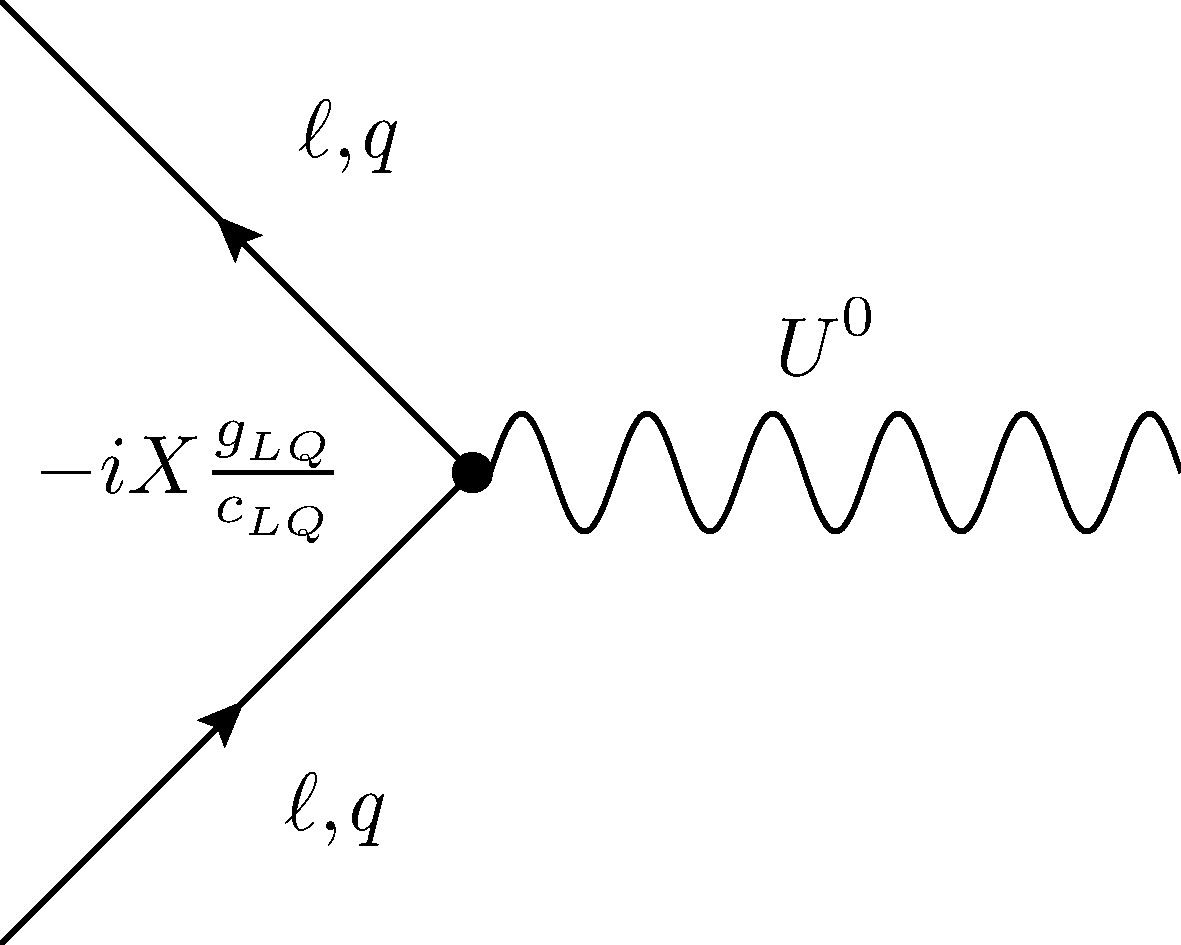
\includegraphics[width= 0.5\textwidth]{./assets/neutral_current}\\\tikzmark{FCNC}  
		\end{center}
		\mycallout<1>{FCNC}{No family-changing neutral current allowed !}
	\end{columns}
	The charged Leptoquark currents \tikzmark{vjcc}  :
	\begin{align*}
		j^{ d CC}_\mu &= \bar \ell \gamma_\mu \omega_L q_{d}  & j^{u CC}_\mu &= \bar \nu \gamma_\mu \omega_L q_{u} 
	\end{align*}
	The neutral Leptoquark currents  \tikzmark{vjnc}  :
	\begin{align*}
		j^{NC}_\mu &= X_\ell\bar \ell \gamma_\mu \ell + X_\nu \bar \nu \gamma_\mu \nu + X_q \bar q \gamma_\mu q. 
	\end{align*}
	\mycallout<1>{vjcc}{$ \mathcal{L}_{cc}= -g_{LQ}j^{ d CC}_\mu V^{-\mu}$}
	\mycallout<2>{vjnc}{$ \mathcal{L}_{nc}= -g'_{LQ}j^{ NC}_\mu U^{\mu}$}
\end{frame}
%%===========================================================
%% Slide 31
%%===========================================================
\begin{frame}{Phenomenology of the model }	
	\begin{columns}[c]
		\column{.5\textwidth}
		\begin{center}
			$ \bar B \to D \ell \bar \nu $ decays \\	
			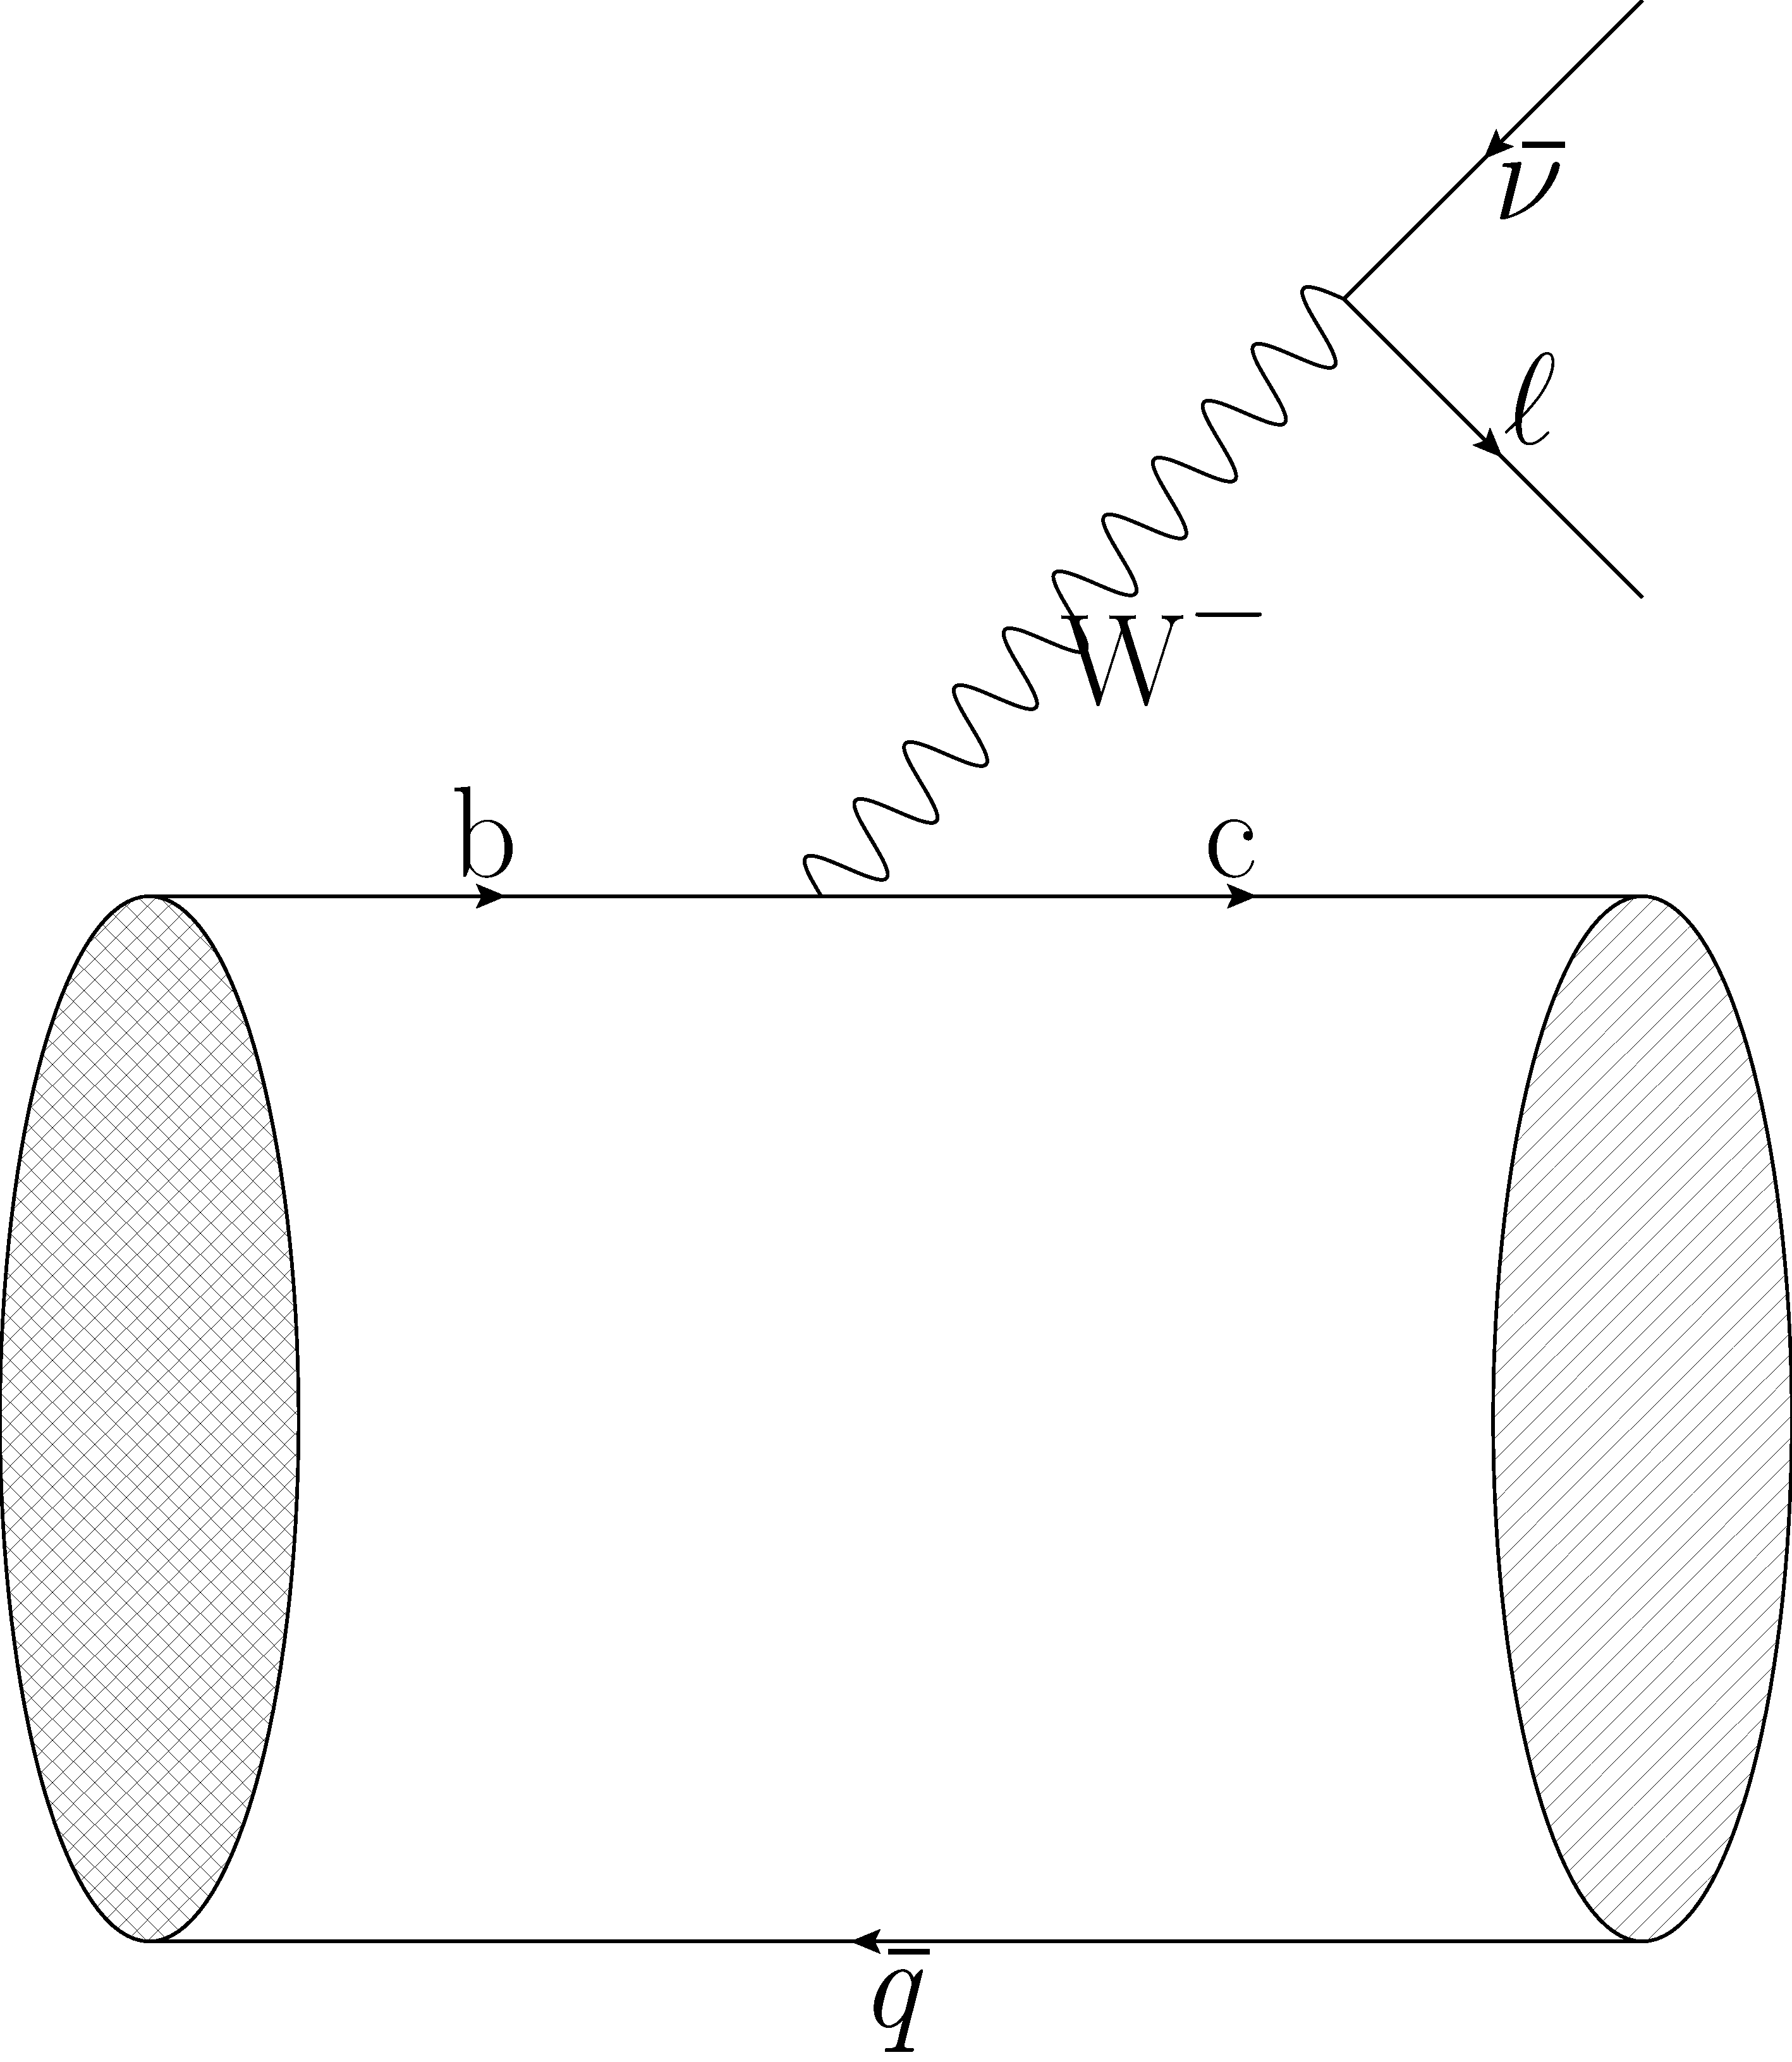
\includegraphics[width= 0.5\textwidth]{./assets/B_to_D_SM} 		\\
			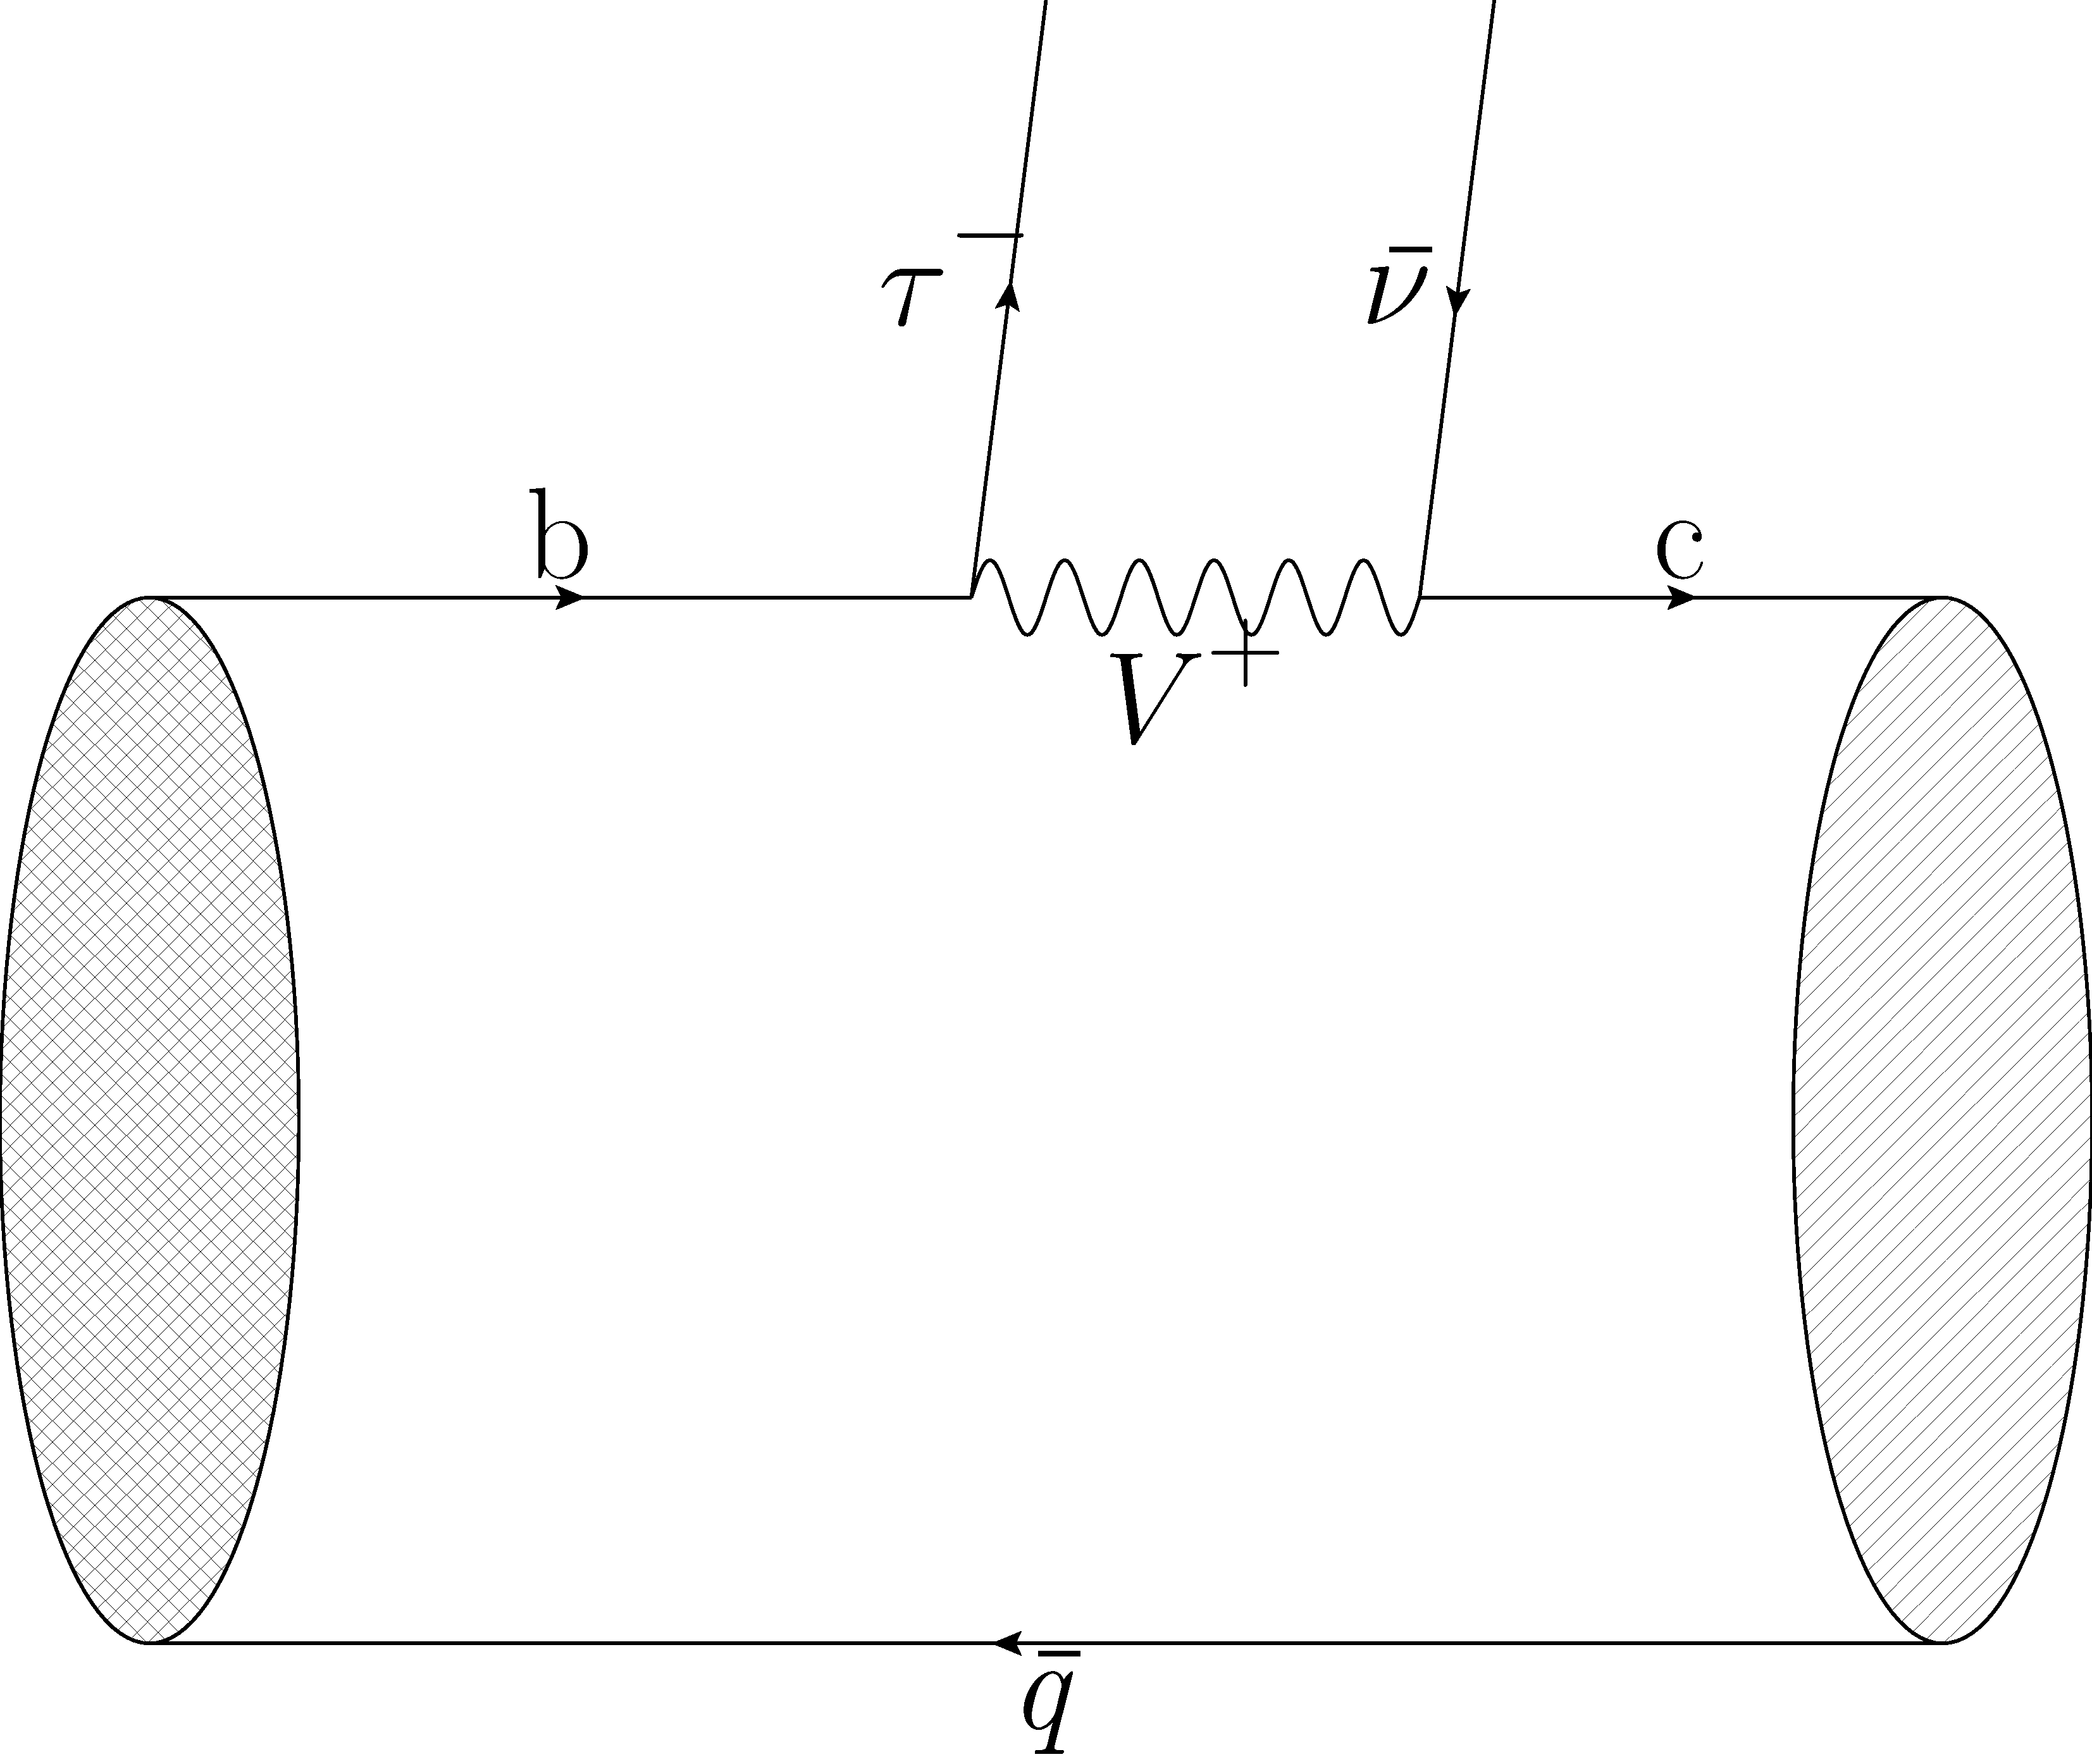
\includegraphics[width= 0.5\textwidth]{./assets/B_to_D_LQ} 	
		\end{center}
		\column{.5\textwidth}
		$ \bar B \to K \ell \bar \ell $ decays \\ 
		\begin{center}
			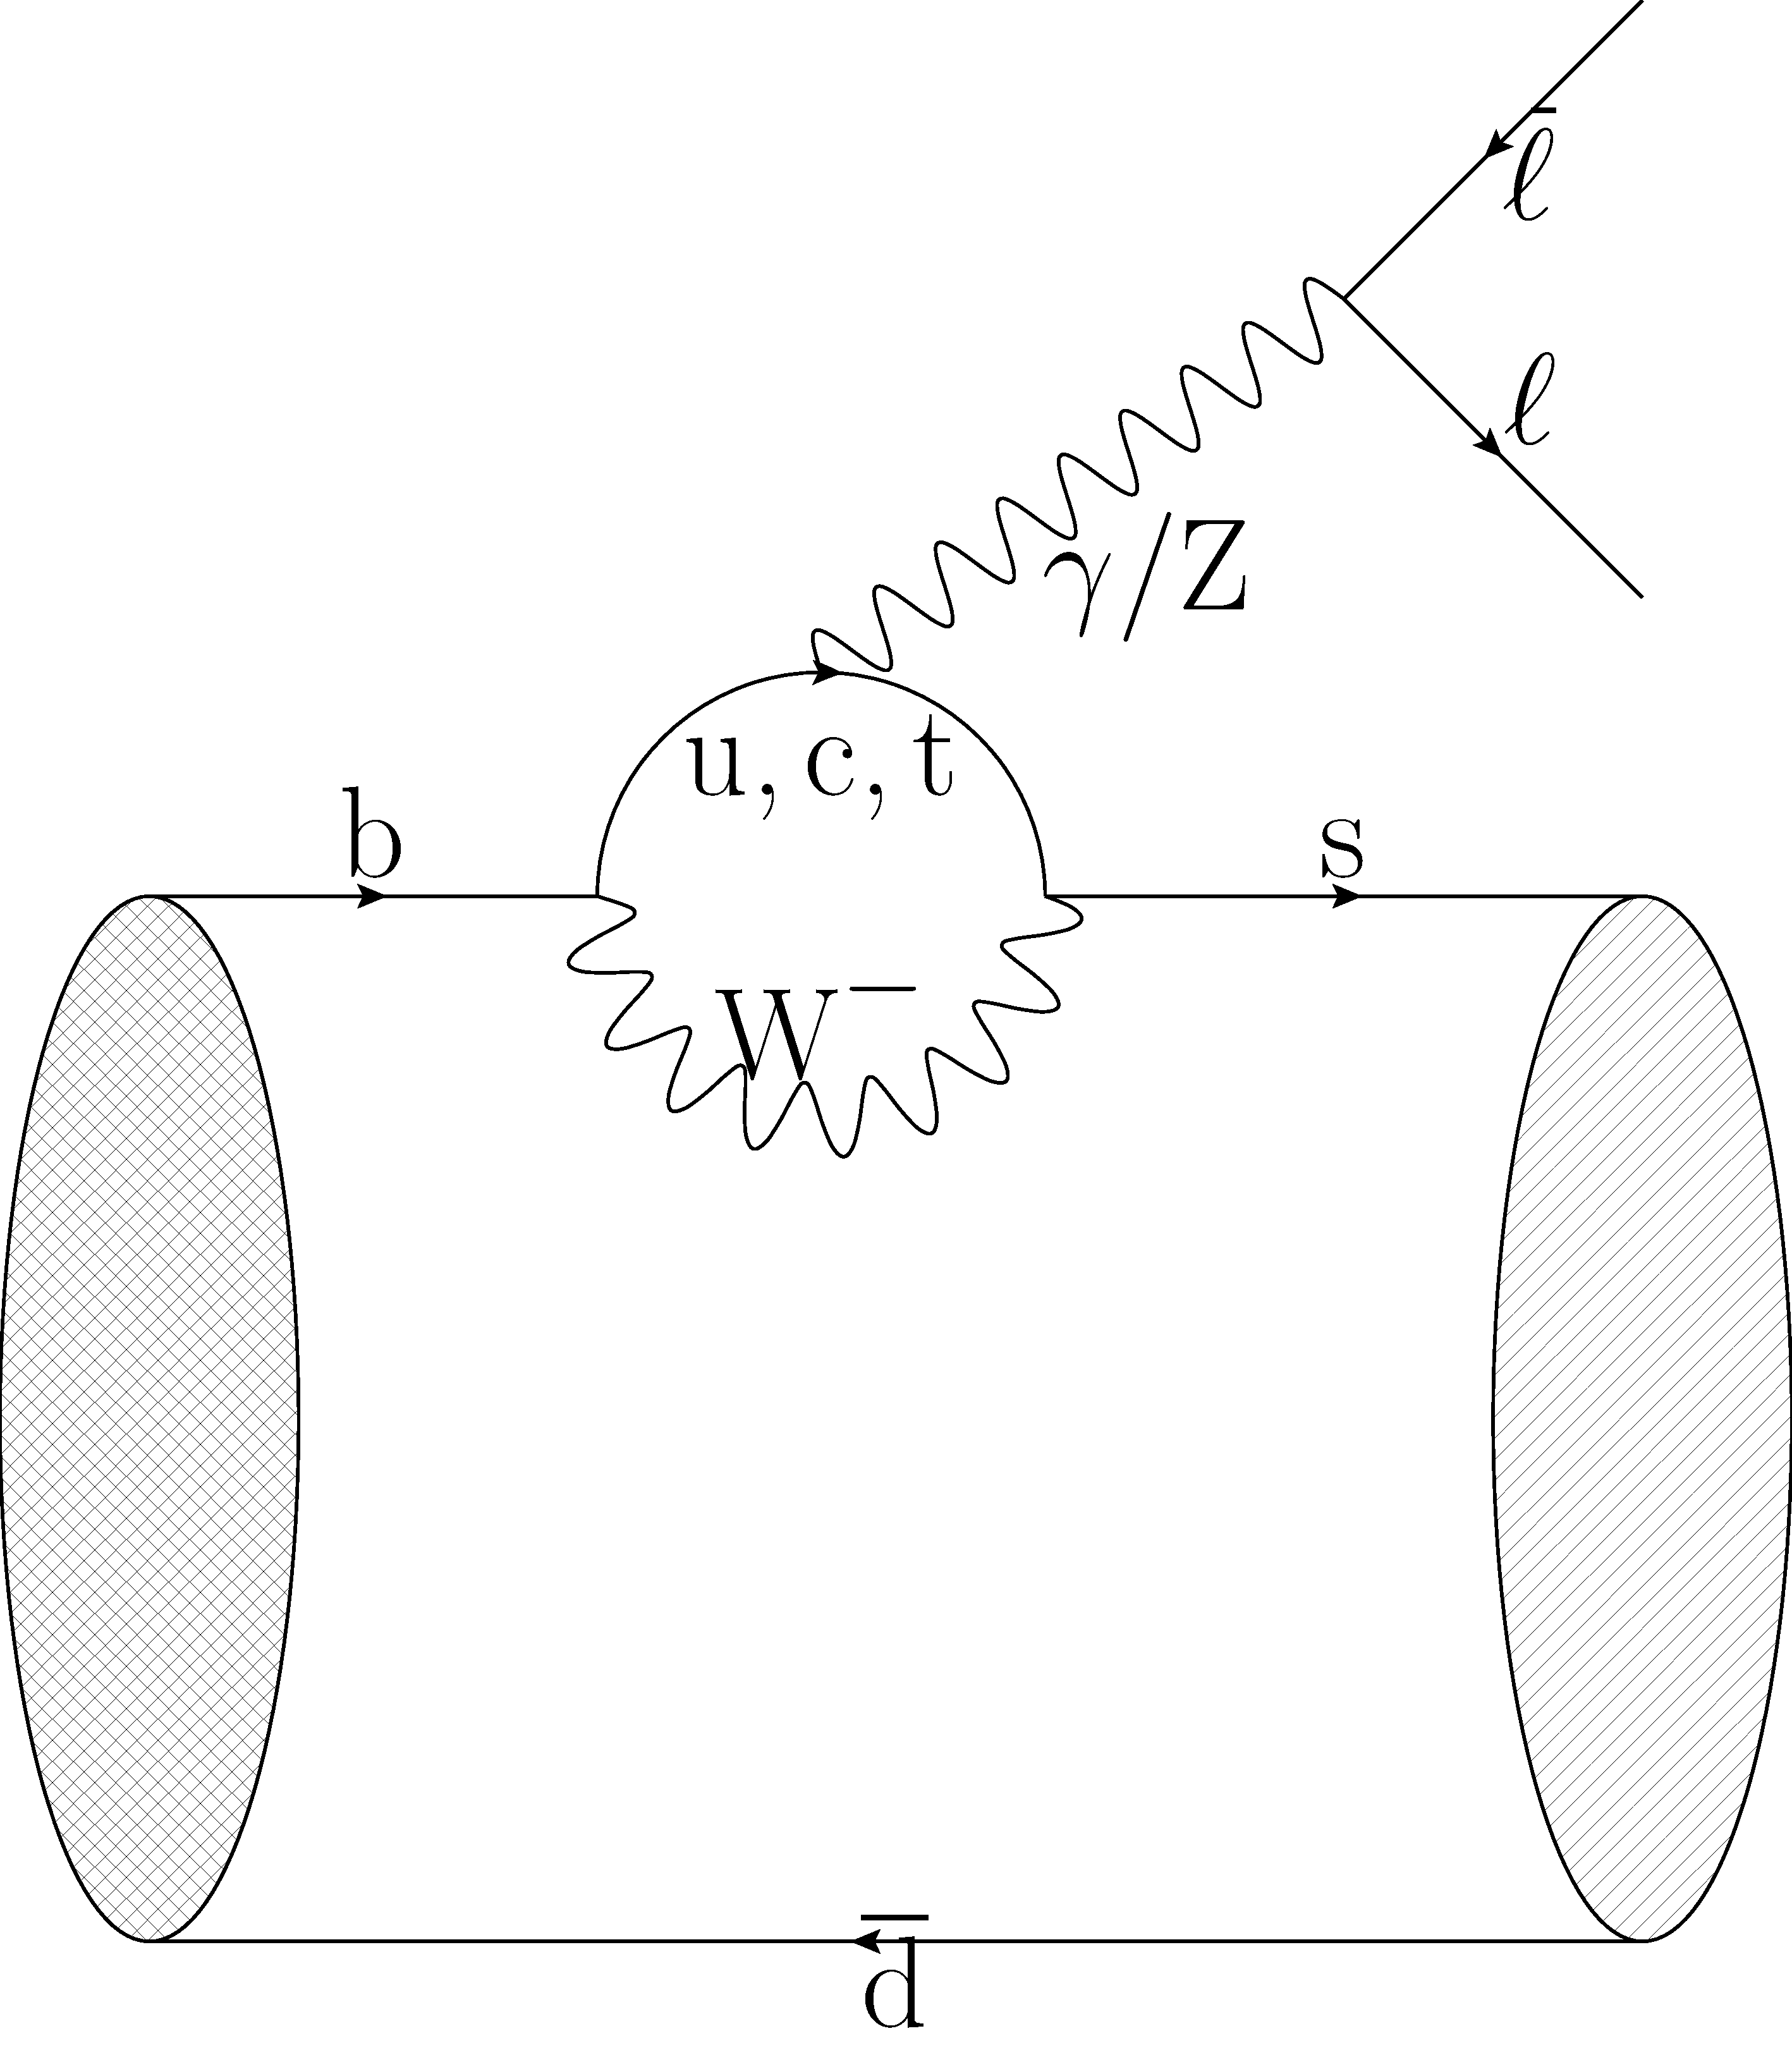
\includegraphics[width= 0.5\textwidth]{./assets/B_to_K_SM} 	\\
			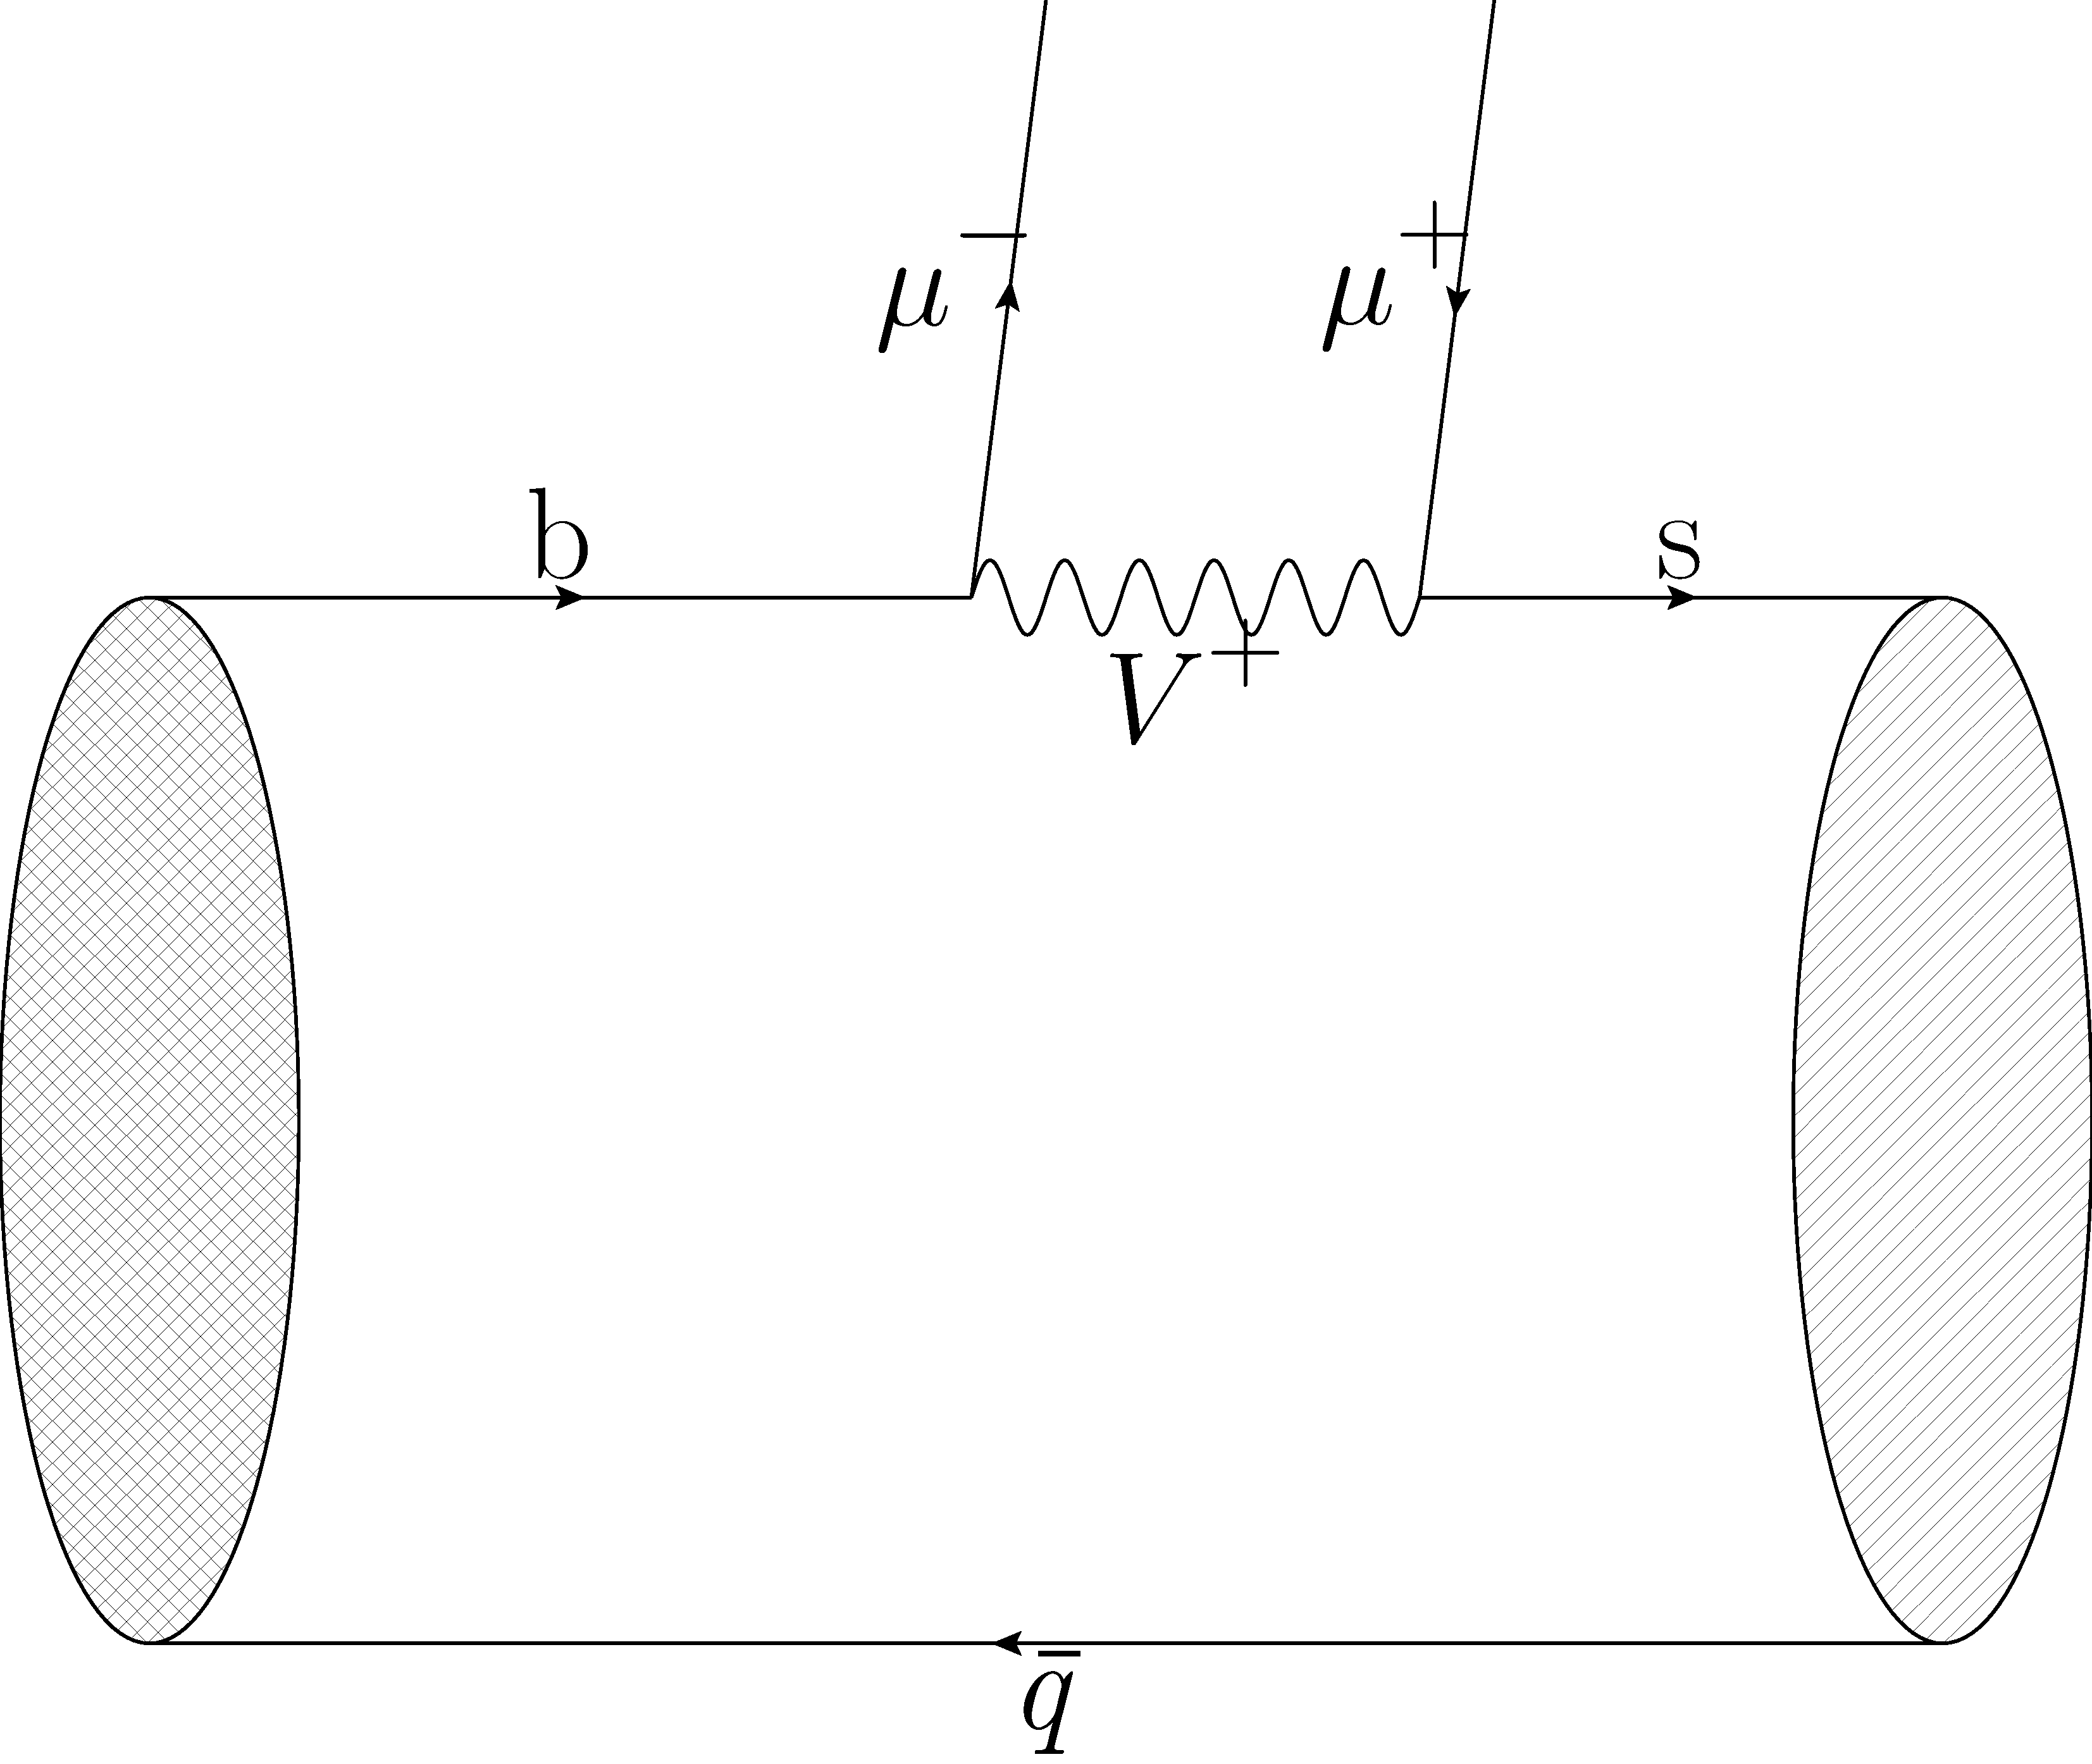
\includegraphics[width= 0.5\textwidth]{./assets/B_to_K_treeLQ}
			%	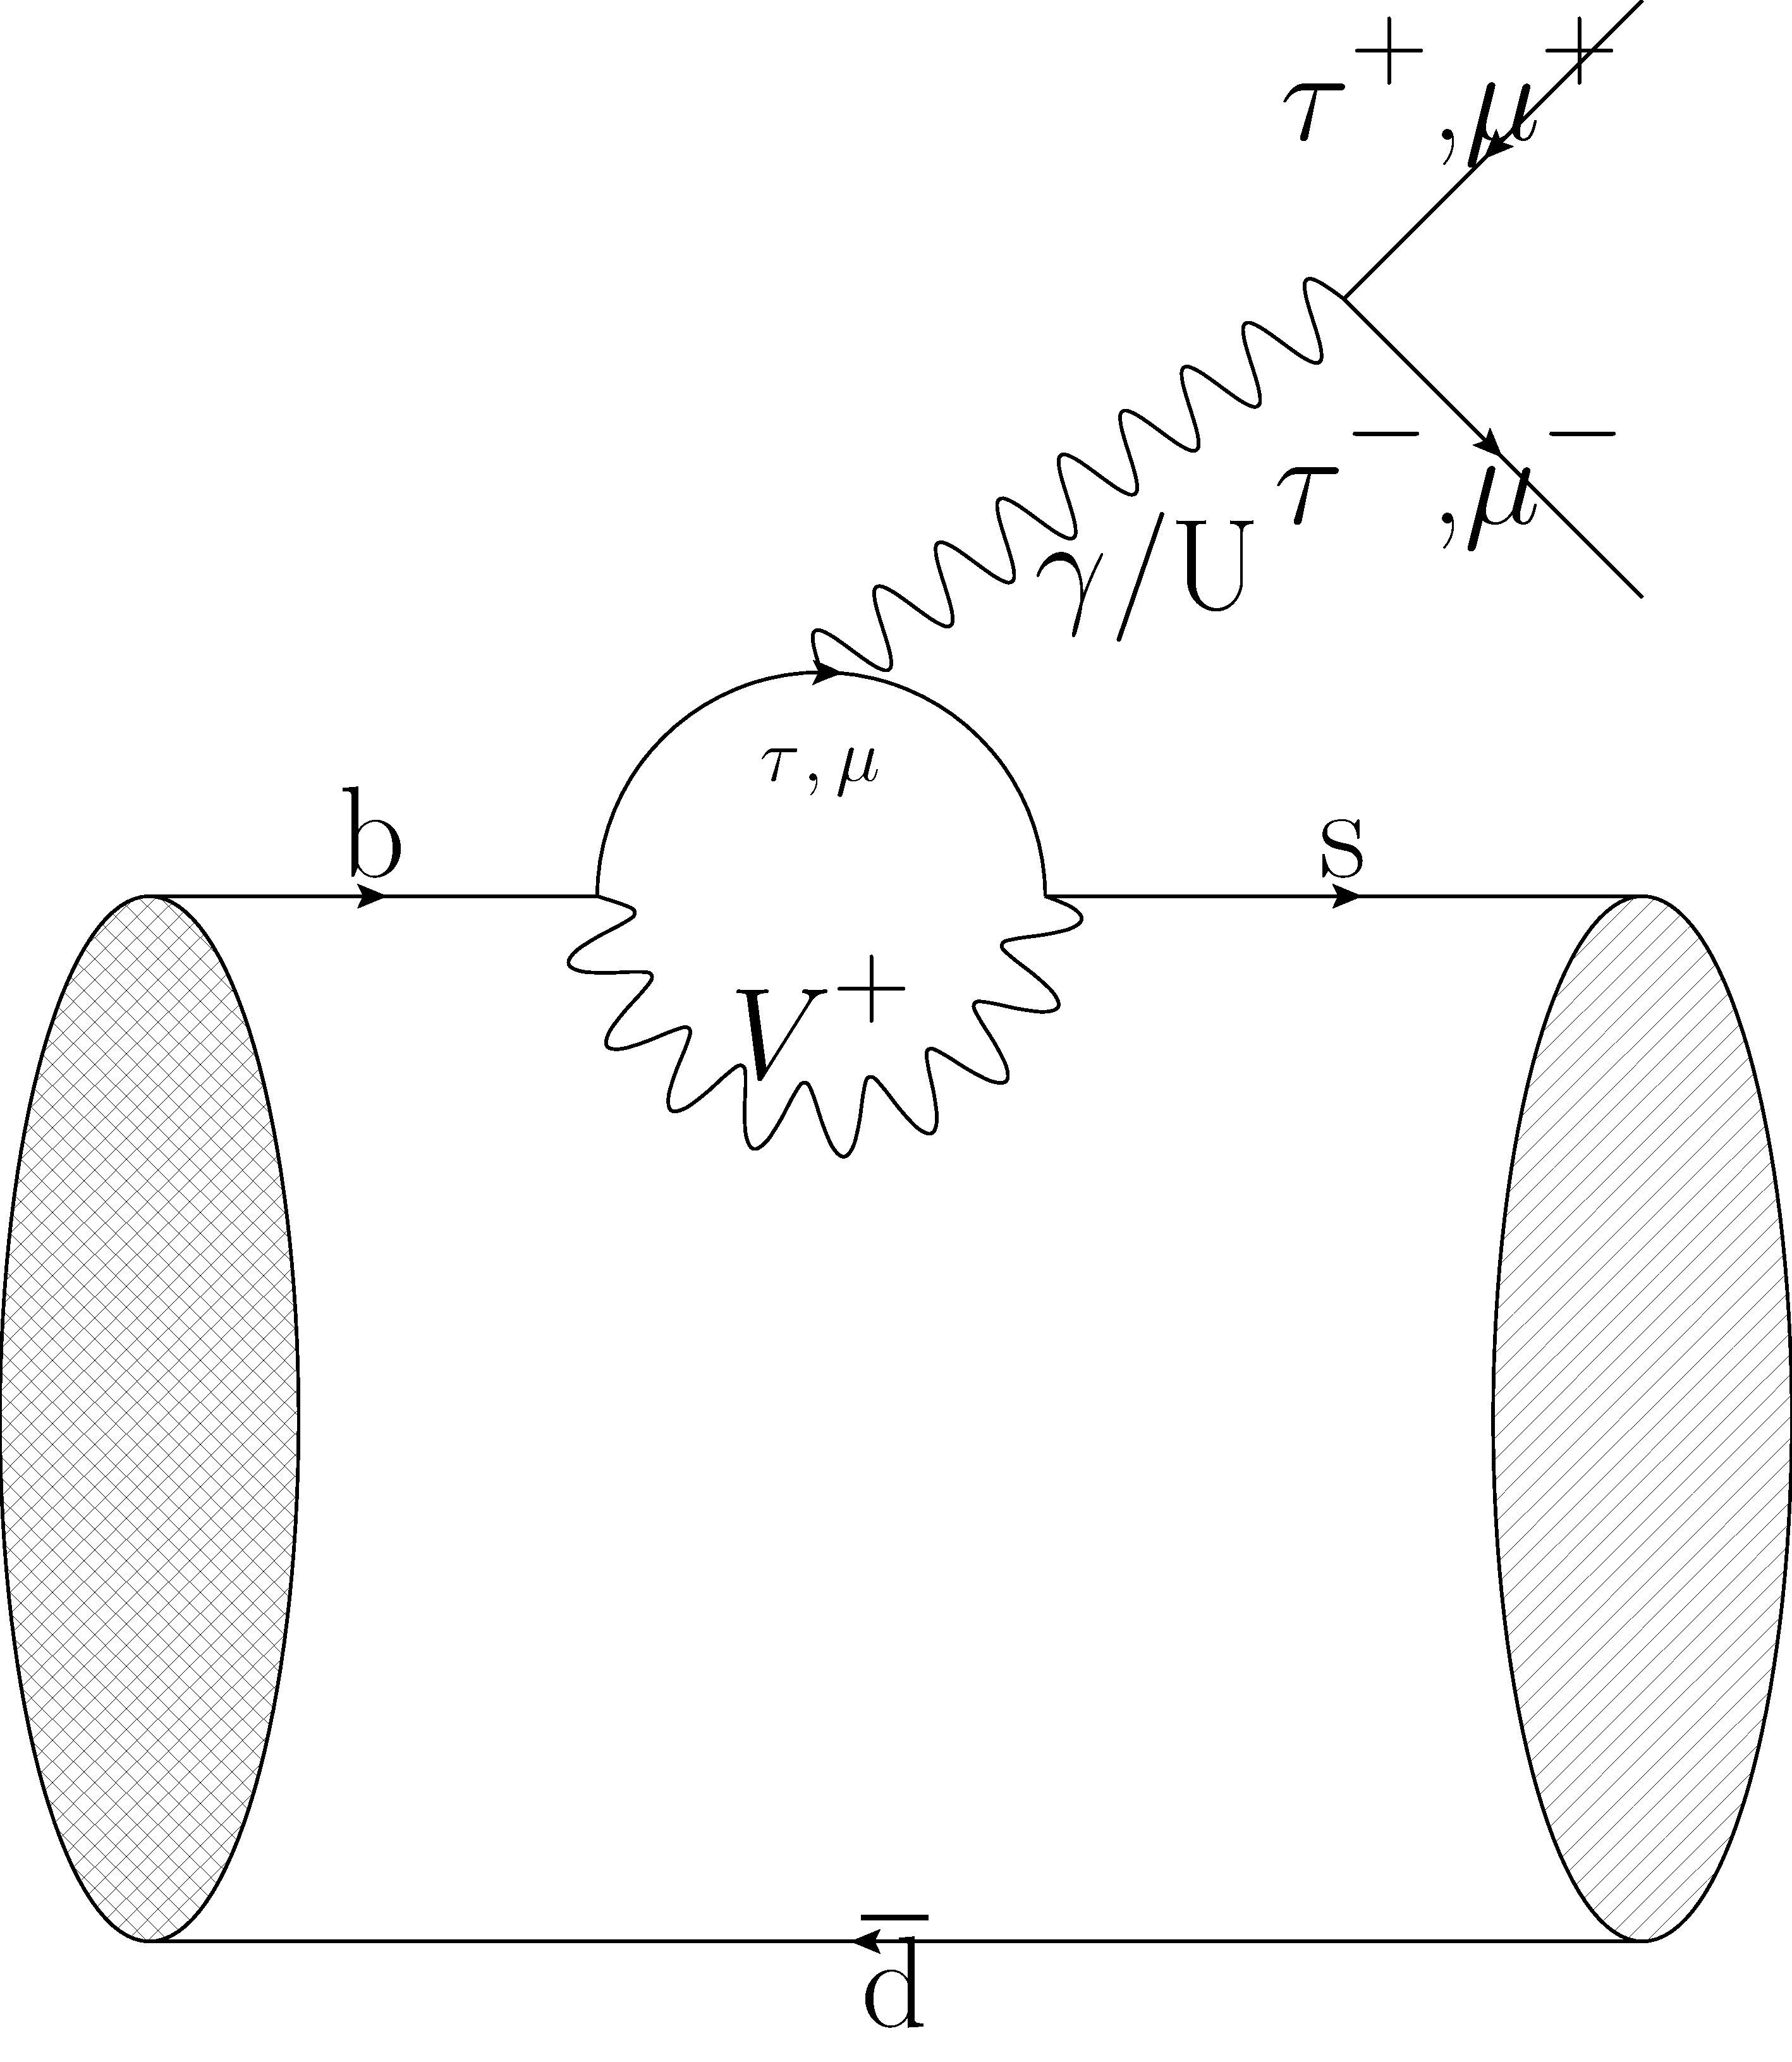
\includegraphics[width= 0.5\textwidth]{./assets/B_to_K_LQ}			
		\end{center}
	\end{columns}
	The transition $ b \to s \mu \mu$ is suppressed by a factor of $\sim 10^{-4}$ although it is at tree-level in this model due to Flavour-mixing.
\end{frame}
%%===========================================================
%% Slide 32
%%===========================================================
\begin{frame}{Direct searches }	
	\begin{columns}[c]
		\column{.5\textwidth}
		\begin{center}	
			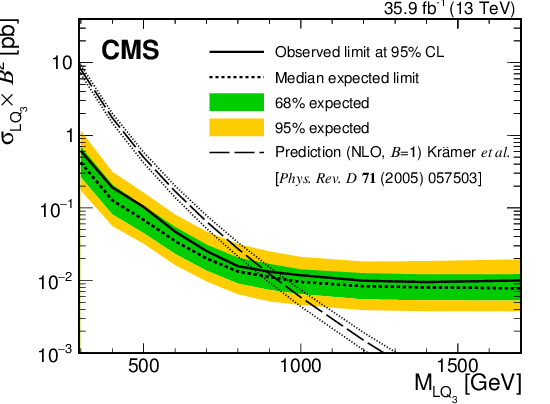
\includegraphics[width=\textwidth]{./assets/lq_cms} 		\\ 3rd gen LQ searches~$M_{LQ}>0.8$\TeV
		\end{center}
		\column{.5\textwidth}

		\begin{center}
			\includegraphics[width= \textwidth]{./assets/zprime_atlas} 	\\ $Z^\prime$-like bosons searches~$M_{Z^\prime}>3.4$\TeV	
		\end{center}
	\end{columns}
\end{frame}
%%===========================================================
%% Slide 33
%%===========================================================
\begin{frame}{Constraints from $\RD$}
	\begin{columns}[c]
		\column{.5\textwidth}
		The Wilson coefficients from the transition $ b\to c \ell \nu$ modified by this model are computed and found to be :
		\begin{align*}
			C^{\tau\nu_\tau}_{VL} &= \beta \frac{\mathcal U_{b\tau} \mathcal U^*_{c \nu_\tau}}{\mathcal{V}^*_{cb}} & C^{\tau \nu_\mu}_{VL} &= \beta \frac{\mathcal U_{b\tau} \mathcal U^*_{c \nu_\mu}}{\mathcal{V}^*_{cb}} \\
			C^{\mu\nu_\tau}_{VL} &= \beta \frac{\mathcal U_{b\mu} \mathcal U^*_{c \nu_\tau}}{\mathcal{V}^*_{cb}} & C^{\mu \nu_\mu}_{VL} &= \beta \frac{\mathcal U_{b\mu} \mathcal U^*_{c \nu_\mu}}{\mathcal{V}^*_{cb}}
		\end{align*}
		with
		\be 
		\beta = \parenths{\frac{g_{LQ}}{g_W}}^2\; \parenths{\frac{M_W}{M_V}}^2 \nonumber
		\ee
		\column{.5\textwidth}
		\begin{center}
			\includegraphics[width= 1.1\textwidth]{./assets/fit_RD} 
		\end{center}
	\end{columns}
	The global fit from experimental data  with $\pm 1 \sigma$ shows a Mass of $3.5$ \TeV\xspace consistent with natural coupling $g_{LQ} \approx 1$
\end{frame}
%%===========================================================
%% Slide 34
%%===========================================================
\begin{frame}{Constraints from $\RK$ and $P^\prime _5$}
	\begin{columns}[c]
		\column{.5\textwidth}
		The Wilson coefficients from the transition $ b\to s \ell \ell$ modified by this model,
		\begin{align*}
		C^{\tau\tau}_{9} &= \beta \frac{\mathcal U_{b\tau} \mathcal U^*_{s\tau}}{\mathcal{V}^*_{tb}\mathcal{V}_{ts}} & C^{\mu\mu}_{9} &= \beta \frac{\mathcal U_{b\mu} \mathcal U^*_{s\mu}}{\mathcal{V}^*_{tb}\mathcal{V}_{ts}}  \\
		C^{\tau\tau}_{10} &=   -C^{\tau\tau}_{9} \\C^{\mu \mu}_{10} &=   -C^{\mu \mu}_{9} 
		\end{align*}
				\column{.5\textwidth}
				\begin{center}
					\includegraphics[width= 1.1\textwidth]{./assets/fit_bsmumu} 
				\end{center}
	\end{columns}
	In order to explain both anomalies, we require that the mixing satisfy~ $\frac{\mathcal U_{b\tau}\,\mathcal U^*_{c \nu_\mu}  }{\mathcal U_{b\mu} \mathcal U^*_{s\mu}}\sim 10^{2}$.
\end{frame}
%%===========================================================
%% Slide 35
%%===========================================================
\begin{frame}{Predictions for $ b \to s \tau \tau$ }
		\begin{columns}[c]
			\column{.5\textwidth}
	\begin{center}
		\includegraphics[width=\textwidth]{./assets/bstautau} 
	\end{center}
			\column{.5\textwidth}
			\begin{center}
				\includegraphics[width= \textwidth]{./assets/Bs_tautau} 
			\end{center}
		\end{columns}	

{\small Enhancement of the branching fractions for the decays involving~$b \tos \tau \tau$ as a function of the LQ flavour mixing., for $M_V \sim 1$ \TeV\xspace and natural coupling. }
\end{frame}
%%===========================================================
%% Slide 36
%%===========================================================
\begin{frame}{What to expect ?}
	\tikzstyle{na} = [baseline=-.5ex]
	The expected  number of $B$'s that are produced at the LHCb and decaying into $ K^* \tau \tau$ with $ \tau \to 3\pi \nu$ and $ \tau \to \mu \nu \bar\nu$ 
	\begin{itemize}[<+-| alert@+>]
		\item  $ 3$ fb$^{-1}$(Run I) \tikz[na] \node[coordinate] (n1) {};  and $ 5$  fb$^{-1}$(Run II).
		
	\end{itemize}
	
	% Below we mix an ordinary equation with TikZ nodes. Note that we have to
	% adjust the baseline of the nodes to get proper alignment with the rest of
	% the equation.
	\begin{equation*}
	\mathcal N = 
	\tikz[baseline]{
		\node[fill=yellow!20,anchor=base] (t1)
		{$\int \mathscr L dt $};
	} \cdot
	\tikz[baseline]{
		\node[fill=orange!20, ellipse,anchor=base] (t2)
		{$\sigma_{b\bar b}$};
	} \cdot
	\tikz[baseline]{
		\node[fill=red!20, ellipse,anchor=base] (t3)
		{$2 f_{b\to B}$};
	} \cdot
	\tikz[baseline]{
		\node[fill=purple!20,anchor=base] (t4)
		{$ 2\mathcal{B}_{B\to K^* \tau \tau} \, \mathcal{B}_{\tau \to 3 \pi \nu} \mathcal{B}_ {\tau \to \mu \nu \bar \nu}$};
	}
	\tikz[baseline]{
		\node[fill=Plum!20, ellipse,anchor=base] (t5)
		{$\varepsilon_{Sel}$};
	}
	\end{equation*}
	
	\begin{itemize}[<+-| alert@+>]
		\item 250$\mu$b$^{-1}$ \@ 13 TeV
		\tikz[na]\node [coordinate] (n2) {};
		\item $\sim 40\%$
		\tikz[na]\node [coordinate] (n3) {};
		\item $\sim10^{-7}$(SM) $\sim10^{-5}$(NP)$ \cdot 0.1 \cdot 0.17$
		\tikz[na]\node [coordinate] (n4) {};
		\item $=\varepsilon_{\text{Acc}}. \varepsilon_{\text{Rec}}. \varepsilon_{\text{Meth}}. \varepsilon_{\text{Trig}}.\varepsilon_{\text{Strip}}. \approx  10^{-6}- 10^{-5}$
		\tikz[na]\node [coordinate] (n5) {};
		\item We get $ \mathcal N \approx 2(SM)-200(NP)$ events \@ Run II of LHCb
	\end{itemize}
	
	% Now it's time to draw some edges between the global nodes. Note that we
	% have to apply the 'overlay' style.
	\begin{tikzpicture}[overlay]
	\path[->]<1-> (n1) edge [bend left] (t1);
	\path[->]<2-> (n2) edge [bend right] (t2);
	\path[->]<3-> (n3) edge [out=0, in=-90] (t3);
	\path[->]<4-> (n4) edge [out=0, in=-90] (t4);
	\path[->]<5-> (n5) edge [out=0, in=-90] (t5);
	\end{tikzpicture}	
\end{frame}
%\begin{frame}{More constraints}
%	
%	\begin{columns}[c]
%		\column{.5\textwidth}
%		Fitting of the lepton mixing~ (PMNS) matrix elements~$\mathcal V _{\tau 3}$ with $M_V=3.5$\TeV\xspace. Shows consistency with current limits from $\nu$ oscillations.
%		\begin{center}
%			\includegraphics[width= 1\textwidth]{./assets/RD_fit_pmns_g.png} 
%		\end{center}
%		\column{.5\textwidth}
%		\begin{center}
%			\includegraphics[width= 1.1\textwidth]{./assets/BR_fit_m_g.png} 
%		\end{center}
%	\end{columns}
%	The global fit from Branching fractions  data  with $\pm 1\sigma$ is again consistent with a Mass of $3.5$ \TeV\xspace consistent with natural coupling $g_{LQ} \approx 1$..
%\end{frame}
%%
%\begin{frame}{The choice of X and anomalies }
%	\begin{columns}[c]
%		\column{.6\textwidth}
%	The choice for the model to be chiral, leaves us with the need to remove the chiral anomalies emerging from triangle diagrams.\\ The convenient choice of $ X= \frac{3Y-T_3}{3}$ is not possible, as the anomaly associated with the  $\SUgroup{2}^2 \Ugroup{1}$ diagram only vanishes when $X_{u}= -X_{d}$. \\ We need to chose $X$ in a different way canceling this anomaly or make the theory couple to both RH and LH chiral fields.
%		\column{.4\textwidth}
%			\begin{center}
%		\includegraphics[width= 0.5\textwidth]{./assets/Triangle_diagram.png} 		 \\ Triangle diagram associated with the chiral anomaly		
%			\end{center}
%
%	\end{columns}
%\end{frame}
%%
%%
%\begin{frame}{Why this model ? }
%\begin{enumerate}
%	\item Simplicity and elegance, assuming a simple group structure with strong link to SM. \pause
%	\item Explaining both $\RK$ and $\RD$, since $b \to s \ell \ell$ could only occur at loop-level, like the SM.\pause
%	\item Adding quark-lepton complementarity to the SM. \pause
%	\item This model is anomaly-free and not an effective theory. \pause
%	\item Interesting scalar sector, needs further investigation. \pause
%	\item Less need for fine-tuning. \pause
%	\item Rich phenomenology, all derived from observation.. \\ B-anomalies, Dark-matter, neutrino mass..etc
%\end{enumerate}
%\end{frame}
\end{document}